\documentclass[12pt,lot, lof]{puthesis}
\newcommand{\proquestmode}{}
% I prefer proquestmode to be off for electronic copies for normal use, since the colored links are less distracting. However when printed in black and white, the colored links are difficult to read. 

\pdfminorversion=4

\title{Wide-area Software-defined Storage}

\submitted{June 2018} 
\copyrightyear{2018} 
\author{Jude Christopher Nelson}
\adviser{Larry Peterson} 
\department{Computer Science}

%%%%%%%%%%%%%%%%%%%%%%%%%%%%%%%%%%%%%%%%%%%%%%%%%%%%%%%%%%%%%\
%%%% Tweak float placements
% From: http://mintaka.sdsu.edu/GF/bibliog/latex/floats.html "Controlling LaTeX Floats"
% and based on: http://www.tex.ac.uk/cgi-bin/texfaq2html?label=floats
% LaTeX defaults listed at: http://people.cs.uu.nl/piet/floats/node1.html

% Alter some LaTeX defaults for better treatment of figures:
    % See p.105 of "TeX Unbound" for suggested values.
    % See pp. 199-200 of Lamport's "LaTeX" book for details.
    %   General parameters, for ALL pages:
    \renewcommand{\topfraction}{0.85}	% max fraction of floats at top
    \renewcommand{\bottomfraction}{0.6}	% max fraction of floats at bottom
    %   Parameters for TEXT pages (not float pages):
    \setcounter{topnumber}{2}
    \setcounter{bottomnumber}{2}
    \setcounter{totalnumber}{4}     % 2 may work better
    \setcounter{dbltopnumber}{2}    % for 2-column pages
    \renewcommand{\dbltopfraction}{0.66}	% fit big float above 2-col. text
    \renewcommand{\textfraction}{0.15}	% allow minimal text w. figs
    %   Parameters for FLOAT pages (not text pages):
    \renewcommand{\floatpagefraction}{0.66}	% require fuller float pages
	% N.B.: floatpagefraction MUST be less than topfraction !!
    \renewcommand{\dblfloatpagefraction}{0.66}	% require fuller float pages

% The documentclass already sets parameters to make a high penalty for widows and orphans. 

\usepackage[utf8]{inputenc}
\usepackage{subcaption}
\usepackage{graphicx}
\usepackage{url}
\usepackage{verbatim}
\usepackage{multirow}
\usepackage{longtable}
\usepackage{booktabs}

%set parameters for longtable:
% default caption width is 4in for longtable, but wider for normal tables
\setlength{\LTcapwidth}{\textwidth}


%%%%%%%%%%%%%%%%%%%%%%%%%%%%%%%%%%%%%%%%%%%%%%%%%%%%%%%%%%
%%% Printed vs. online formatting
\ifdefined\printmode

% Printed copy
% url package understands urls (with proper line-breaks) without hyperlinking them
\usepackage{url}


\else

\ifdefined\proquestmode
%ProQuest copy -- http://www.princeton.edu/~mudd/thesis/Submissionguide.pdf

% ProQuest requires a double spaced version (set previously). They will take an electronic copy, so we want links in the pdf, but also copies may be printed or made into microfilm in black and white, so we want outlined links instead of colored links.
\usepackage{hyperref}
\hypersetup{bookmarksnumbered}

% copy the already-set title and author to use in the pdf properties
\makeatletter
\hypersetup{pdftitle=\@title,pdfauthor=\@author}
\makeatother

\else
% Online copy

% adds internal linked references, pdf bookmarks, etc

% turn all references and citations into hyperlinks:
%  -- not for printed copies
% -- automatically includes url package
% options:
%   colorlinks makes links by coloring the text instead of putting a rectangle around the text.
\usepackage{hyperref}
\hypersetup{colorlinks,bookmarksnumbered}

% copy the already-set title and author to use in the pdf properties
\makeatletter
\hypersetup{pdftitle=\@title,pdfauthor=\@author}
\makeatother

% make the page number rather than the text be the link for ToC entries
%\hypersetup{linktocpage}
\fi % proquest or online formatting
\fi % printed or online formatting


%%%%%%%%%%%%%%%%%%%%%%%%%%%%%%%%%%%%%%%%%%%%%%%%%%%%%%%%%%%%%\
%%%% Define commands

% Define any custom commands that you want to use.
% For example, highlight notes for future edits to the thesis
%\newcommand{\todo}[1]{\textbf{\emph{TODO:}#1}}


% create an environment that will indent text
% see: http://latex.computersci.org/Reference/ListEnvironments
% 	\raggedright makes them left aligned instead of justified
\newenvironment{indenttext}{
    \begin{list}{}{ \itemsep 0in \itemindent 0in
    \labelsep 0in \labelwidth 0in
    \listparindent 0in
    \topsep 0in \partopsep 0in \parskip 0in \parsep 0in
    \leftmargin 1em \rightmargin 0in
    \raggedright
    }
    \item
  }
  {\end{list}}

% another environment that's an indented list, with no spaces between items -- if we want multiple items/lines. Useful in tables. Use \item inside the environment.
% 	\raggedright makes them left aligned instead of justified
\newenvironment{indentlist}{
    \begin{list}{}{ \itemsep 0in \itemindent 0in
    \labelsep 0in \labelwidth 0in
    \listparindent 0in
    \topsep 0in \partopsep 0in \parskip 0in \parsep 0in
    \leftmargin 1em \rightmargin 0in
    \raggedright
    }

  }
  {\end{list}}



%%%%%%%%%%%%%%%%%%%%%%%%%%%%%%%%%%%%%%%%%%%%%%%%%%%%%%%%%%%%%\
%%%% Front-matter

% For early drafts, you may want to disable some of the frontmatter. Simply change this to "\ifodd 1" to do so.
\ifodd 0
% front-matter disabled while writing chapters
\renewcommand{\maketitlepage}{}
\renewcommand*{\makecopyrightpage}{}
\renewcommand*{\makeabstract}{}

% you can just skip the \acknowledgements and \dedication commands to leave out these sections.

\else


\abstract{
% Abstract can be any length, but should be max 350 words for a Dissertation for ProQuest's print indicies (150 words for a Master's Thesis) or it will be truncated for those uses.
The proliferation of commodity cloud services helps developers build
wide-area ``system-of-systems'' applications by harnessing
cloud storage, CDNs, and public datasets as reusable building blocks.
But to do so, developers must contend with two
long-term challenges.  First, whenever developers change storage providers, 
they must work to preserve the application's expected \emph{storage
semantics}, i.e. the rules governing how the application expects the
storage provider to handle its reads and writes.  Today, changing
storage providers is costly, because developers need to patch
the application to make it compatible with the new provider's
data consistency model, access controls, replica placement
strategies, and so on.

At the same time, users have certain expectations about how their
data will be used, which the application must meet.
For example, depending on the application, users
may expect that their data will be kept private from other users, that their data will be exportable
to other applications, that accesses to their data will be logged in an auditable way,
and so on.  In the limit, each user's expectations represent an implicit
\emph{policy} constraining how their data can be stored.  Honoring
these policies is difficult for developers who rely on third-party storage
providers because the storage provider is often unaware of them.

This thesis addresses these challenges with a wide-area storage protocol, called ``software-defined
storage'' (SDS), that runs in-between applications and cloud services.
SDS-enabled applications do not host data, but instead let users
bring their preferred cloud services to the application.  By taking a
user-centric approach to hosting data, users are empowered to programmatically
specify their policies independent of their applications and select
services that will honor them.  To support this approach and to
tolerate service provider changes, SDS empowers developers to programmatically
specify their application's storage semantics independent of storage providers.

This thesis presents the design principles for SDS, and validates their
real-world applicability with two SDS implementations and several non-trivial
applications built on top of them.  Most of these applications are used in
production today.  This thesis
presents early performance results of its SDS implementations and uses
real-world experiences to show how to make the most of SDS.

}

\acknowledgements{
% TODO intro
The work presented in this thesis is drawn from two major collaborations.
One was with Princeton, the University of Arizona, and the University of North Carolina, 
and the other was with Blockstack Public Benefit Corporation (PBC).

The first body of work was conducted in the PlanetLab research
group, later as part of OpenCloud, and finally as part of a NSF grant shared by
Princeton, UA, and UNC.  The project that began as
protocol to turn a commodity content distribution network (CDN) into a write-coherent 
network cache ultimately evolved into Syndicate, the first wide-area
software-defined storage system.  I am grateful to my advisor Larry L. Peterson
for taking me under his wing and guiding me on the path that led to this
thesis, and I am grateful to have been mentored by 
PlanetLab researchers Sapan Bhatia, Andy Bavier, Mike Wawrzoniak, Marc
Fiuczynski, Tony Mack, and Scott Baker---all of whom played a part in navigating
graduate school in my earlier years at Princeton.

It takes a lot of engineering work and attention to
detail to make a project of Syndicate's scope operational.
During my time with PlanetLab and OpenCloud, I worked with many talented people
at Princeton and the University of Arizona who helped 
see this task through to completion.  I am grateful to Illyoung Choi for helping me get
Syndicate to work in production settings.  He made Syndicate compatible with Hadoop,
he wrote drivers for public datasets and iRODS, he filmed video tutorials 
for using Syndicate, and he created Docker images and dataset mounting tools
that make Syndicate easy to use.  He was also instrumental in discovering,
reproducing, and gathering logs for countless bugs.

In addition, I am grateful to Zack Williams
for creating and running Syndicate's continuous integration and packaging
infrastructure, and I am grateful to Jack L. Pogue III for writing
and maintaining the Syndicate test suite and creating manual pages for all of
the Syndicate programs.  Their efforts significantly improved the developer
experience for hacking on and using Syndicate.
I would also like to thank Muneeb Ali, Wathsala Vithanage,
and John Whelchel for working on Syndicate with me in the summer of 2013,
and I would like to thank Nirav Merchant and Bonnie Hurst
for giving us the chance to use Syndicate on real-world scientific workflows.
Wathsala Vithanage also deserves credit for helping create an end-to-end
encrypted email application on top of Syndicate.

The other body of work was conducted with Blockstack,
a public benefit corporation started by Muneeb Ali `17 and Ryan Shea
`12.  At Blockstack, I developed the first version of Gaia---a wide-area
software-defined storage system for Web applications.  A key discovery that
made Gaia possible was the invention of a technique called \emph{virtualchains},
which allow Syndicate and Gaia to leverage an existing cryptocurrency blockchain to
implement public-key infrastructure.  I have Muneeb and Ryan to thank for
helping me overcome my (deep) skepticism of
the usefulness of blockchains, and for allowing me to work on Gaia as a
collaborative work with Princeton.  In addition, I would like to thank Michael
J. Freedman for advising the three of us on the design and implementation of
this system.

Gaia today sees widespread use in Blockstack's application ecosystem as the
\emph{de facto} storage system.  I am especially thankful to have worked with
Blockstack engineers Aaron Blankstein, Larry Salibra, Ken
Liao, Jack Zampolin, Chase Wackerfuss, Thomas Osmonson, and Sebastian Dunkel for
helping make this happen, and I'm thankful to all of the Blockstack developers
and community members who built real-world applications with Gaia and helped us
find bugs and improve the system.

This thesis took a longer route than usual because it spanned two separate
efforts.  I would like to thank my thesis committee members Jennifer Rexford,
John H. Hartman, Brian W. Kernighan, and Kai Li for their invaluable feedback on
this work.  I would also like to thank my partner Meghan who helped me stay
encouraged to work on this thesis when I was
struggling.  Finally, I would like to thank my parents Mark and Monica for
instilling within me a lifelong passion for learning and a sense of
self-motivation to see it through.

Parts of this thesis were published earlier in the following papers:

\begin{itemize}
\item Jude C. Nelson and Larry L. Peterson. \emph{``Syndicate: Virtual Cloud
Storage through Provider Composition.''} In Proceedings of the 2014 ACM
International Workshop on Software-defined Ecosystems (BigSystem '14).
ACM, New York, NY, USA, 1-8.
\item Muneeb Ali, Jude Nelson, Ryan Shea, and Michael J. Freedman.
\emph{``Blockstack: A Global Naming and Storage System Secured by
Blockchains,''} 2016 USENIX Annual Technical Conference, Denver, CO, June 2016.
\item Jude Nelson, Muneeb Ali, Ryan Shea, and Michael J. Freedman.
\emph{``Extending Existing Blockchains with Virtualchain,''} Workshop on
Distributed Cryptocurrencies and Consensus Ledgers, Chicago, IL, July 2016.
\item Muneeb Ali, Jude Nelson, Ryan Shea, and Michael J. Freedman.
\emph{``Bootstrapping Trust in Distributed Systems with Blockchains,''}, USENIX
;login: Issue: Vol 41, No. 3, Pages 52-58, Fall 2016.
\end{itemize}

I was supported by a Princeton Graduate Fellowship in my first year at
Princeton.  I was hired by Princeton University for the academic year 2014-2015
to work as a research technician on making Syndicate an operational service for
the OpenCloud project.  The work on Syndicate was supported by NSF Award 1541318.

}

\dedication{For Mark, Monica, Luke, and Meghan}

\fi  % disable frontmatter


\begin{document}

\makefrontmatter

\chapter{Introduction}
\label{chap:introduction}

The proliferation of cloud-based services poses new opportunities and
challenges for hosting data.  On the one hand, the availability of
professionally-maintained infrastructure is a boon to developers, since it
offloads a large operational burden for maintaining user data.  On the other
hand, developers find themselves having to leverage multiple services in a way
that both preserves their end-to-end storage requirements while
avoiding vendor lock-in.  This thesis presents and evaluates a new storage
architecture for overcoming this challenge in the context of two classes of
networked application: scientific computing workflows and decentralized
applications.

Scientific computing workflows and decentralized applications may
serve wildly different use-cases, but they operate under similar data-hosting
conditions.  First, they store and share data across multiple organizational
domains, such as different user groups, university networks, corporations, and
legal jurisdictions.  Second, each organizational domain has its own requirements
on how its users should store their data and make it available to others.  Third, data
management responsibilities in the application are distributed, where each
domain acts semi-autonomously.  There is no clear "application data owner" that unilateraly
decides hosting policies for all participants.

In practice, these applications are systems-of-systems, and stand to benefit
from leveraging existing systems instead of building new, bespoke ones from
scratch.  An application can make use of one or more \textbf{cloud storage}
providers to host its users' data,
and can distribute it to a scalable number of readers via one or more \textbf{content
distribution networks} (CDNs).  In addition, it can leverage data from
one or more external \textbf{curated data-sets} to provide better value to users.
For example, a navigation application like OpenStreetMap~\cite{openstreetmap} would host its users'
preferred routes, maps, and historic queries to the storage providers of their choice,
use a CDN to pre-fetch and cache map data to its appropriate geographic regions,
and use public weather data aggregated by NOAA to predict how long a commute may take.

The benefit to developers is obvious.  By relying on existing infrastructure,
they can reduce development time and focus primarily on their application's business
logic.  In a competative domain, this translates to reducing time-to-market,
and can make the difference between an application's success or failure.

However, there are two long-term risks with this strategy.  First, these
services are fundamentally unreliable.  They can unilaterally
change their pricing, feature-set, APIs, and availability.
Applications that rely on these services can break without warning,
and cost developers unforeseeable amounts of time and money.

Second, these services are heterogeneous.  Services that fill a similar role
do not offer uniform interfaces or well-defined semantics.
Without careful planning, the application will become tightly-coupled to the
services it uses by depending on it to behave a certain way (even if this
dependency is implicit).  This creates high infrastructure switching costs, making it
difficult for developers to address service unreliability or move to better
offerrings.

Designing applications to be portable mitigates both of
these risks.   However, the cost of porting $m$ applications to $n$ services
today requires $O(mn)$ patches.  This is true even if developers share their
patches---getting a patch to work with one application rarely requires zero
edits to work with another.  We do not believe this situation
will improve, since developers are compensated for shipping working
code rather than portable code.

Our solution is to port both applications and services to a shared
intermediate layer called a \emph{software-defined storage} (SDS) system.
This allows developers to ignore service-specific compatibility, and allows service
operators to \emph{port services to applications} by making them compatible with
the SDS system.  In doing so, we bring the portability cost down from
$O(mn)$ to $O(m + n)$ patches while preserving the application's end-to-end
storage requirements.

We achieve this with a shared layer of indirection.  Instead of focusing on
porting each application to each service, we focus on porting applications and
services to an intermediate layer.  We will have this intermediate layer mediate all
data interactions between applications and services.  The goal is that when a new service
is ported to this layer, all existing applications can make use of it without
modification.  We call a system that implements this layer a
\textit{wide-area software-defined storage} (SDS) system.

Wide-area SDS is unique in how it addresses application/service compatibility.
Unlike existing service compatibility frameworks, it focuses on preserving
the application's desired end-to-end storage semantics
irrespective of the underlying services' semantics.  Our prototype
system, called Syndicate, gives application end-points a coherent read/write
filesystem view of their data and offers developers a UNIX-y programming model
for describing the storage semantics their applications need.  In doing so, we
reduce the global number of portability patches from $O(mn)$ to $O(m + n)$.

\section{Contributions}

This thesis makes the following contributions:

\begin{itemize}

\item We present the design principles of software-defined storage, framed in
terms of prior work and the real-world storage needs of both scientific
workflows and decentralized applications.  We show how to
keep the number of portability patches limited to $O(m + n)$ while
both preserving end-to-end storage semantics and
respecting each organization's data-hosting policies
(Chatper~\ref{chap:design_principles}).

\item We present the design and implementation of Syndicate, a file-oriented SDS
system.  Syndicate is a real SDS system being deployed in scientific workflows today.
We show how Syndicate makes use of SDS design principles, and discuss lessons
learned in implementing SDS (Chapter~\ref{chap:syndicate_sds}).
We also show early performance numbers (Chapter~\ref{chap:evaluation}).

\item We show how to build SDS-powered applications.  We present the design and
implementation of three non-trivial applications on top of SDS: email, encrypted
file sharing, and automatic HPC data staging.  We show how each system can be
implemented on top of SDS such that each one reuses the same $n$
service-specific patches while requiring only a modest amount of
application-specific code for preserving storage semantics
(Chapter~\ref{chap:applications}).

\end{itemize}


\chapter{Design Principles of Software-defined Storage}
\label{chap:design_principles}

This chapter presents the design
principles of SDS using real-world observations of contemporary
system-of-systems applications.
It describes the components that make up an SDS system
and shows how they work together to preserve end-to-end semantics while
preserving organizational autonomy.

\section{Overview}

The need for SDS systems is guided by the real-world needs of three sets of stakeholders in
wide-area applications today:  its users, its organizations, and its developers.

\subsection{Users}

The \textbf{users} are the authoritative origins of all data in the application.
Data is produced by users for other users to consume.  This is unsurprising at
first glance, since the point of having wide-area applications at all is so users can
collaborate without having to be physically present 
(i.e. by communicating data to one another across the Internet).  However, the
key insight here is that conventional wide-area applications such as Web
applications do not treat users as authoritative data origins at the protocol
level.  At the protocol level, application servers are the authoritative data origins for
all user data. 

It is only by \emph{social convention} that users are led to believe and
expect that they are the authoritative data origins.  This is reflected in how
users talk about the data they create---for example, a user would say ``my
Facebook profile'' when referring to the profile data Facebook hosts, instead of the more accurate
statement ``the downstream replica of my profile data that I stored in Facebook's servers and
expect Facebook's servers to faithfully share on my behalf.''
This thesis argues for enforcing this
social convention at the protocol layer (i.e. programmatically, beneath the application)
by separating the responsibility for hosting
and serving a user's data from the responsibility of hosting and running
application code.

The fact that users assume that they are both
the data's authoritative origins and the data consumers
means that users have certain expectations regarding how applications store
their data.  These expectations can be arbitrarily specific to the data, the application, and the
computer(s) through which they read and write it.  For example, a user would
expect an online tax-filing application to prevent their tax form data from being read by anyone
besides themselves and the government, and would expect it to retain copies of their 
filings for at least three years.  As another example, a user would expect a
ride-hailing application to be accessible only through their mobile phone, and
would expect that their travel history and driver ratings would be inaccessible
to the driver.

\subsubsection{Data-hosting Policies}

Successful applications empower users to convey their expectations to
applications and other users in the form of a \textbf{data-hosting policy}.
The data-hosting policy is a machine-readable
description of how the user expects application and other users to interact
with her data.  Successful applications provide the means for users to translate their
expectations into data-hosting policies, and enforce the users'
policies on their behalf behalf.

The data-hosting policy can take many forms, depending on the application.
For example, a social media application like Facebook allows
users to encode some aspects of a data-hosting policy in a privacy settings page.
The settings are stored in Facebook, and Facebook (obstensibly) enforces them.
As another example, a cloud administration tool like the Google Cloud
Console~\cite{google-cloud} gives its users the ability to define programmatic
hooks and scripts for hosting, retaining, and deleting log data.

This thesis is concerned about the enforcement of data-hosting policies.
Users need to be able to translate their expectations on data storage into
policies that they can enforce without having to rely on applications or storage
providers.  Today, users have no technical recourse if the application
simply decides to ignore their policies; they are instead left with external
remediation options like boycotting the application or taking legal action
against the developers.  Specific to system-of-systems applications,
developers are not in a position where they can plausibly enforce a user's data-hosting
policies end-to-end.  This is because in order to do so, 
both the application and the storage
providers must recognize and enforce the users' policies.  However, in practice storage
providers are not even guaranteed to be aware that the policies exist,
since users do not interact with storage providers and do not have a direct business
relationship with them.

If users cannot rely on the application or the developer's chosen storage providers
to enforce their data-hosting policies, then they they are left with three
(non-exclusive) options:

\begin{enumerate}
   \item Do not use the application.  This is not a feasible option for
      most users.
   \item Only use the application if it will store the user's data on the user's
      chosen storage providers, instead of the developer's.  That
      way, the user can obstensibly select storage providers that will enforce 
      their policies alongside the application.
   \item Carry out policy enforcement on a trusted computer or computers
      independent of the application and storage providers.
\end{enumerate}

This thesis argues for taking the second and third options in system-of-systems
application design.  Users should be able to
bring their preferred storage providers to the application, and entrust
data-hosting policy enforcement with the organizations of their choosing.
Applications and storage providers should not be trusted with doing so.

\subsection{Organizations}

An \textbf{organization} is the set of computers that implement a user's
data hosting policy.  Each organization adheres to a single
policy, and uses it to constrain how the application and other users are allowed to
interact with the user's data.

The fact that policies are application-specific means that organizational boundaries
are also specific to the application, since they pertain to the types of data being loaded
and stored in the application.  Examples of organizations include:

\begin{itemize}
   \item A user's personal devices constitute a single organization in the context of a
      social media application.  This is a single organization because all
      devices adhere to the same data-hosting policy:  they load, manipulate,
      and store the user's account and profile data.  Organizations do not
      overlap in this application---a user Alice's devices are a wholly
      separate organization from a user Bob's devices.
   \item A lab's workstations constitute a single organization in the context of
      a Web BLAST~\cite{web-blast} deployment.  This is a single organization
      because all hosts adhere to the same access controls:  only lab members
      can access unpublished data, and only a lab member and the site
      administrator can access user-specific state like home directories.
      However, labs can share public data through the Web BLAST instance with
      one another.
   \item A set of users' personal devices constitute a single organization in
      the context of a shared version control system (VCS).  Each user can access the
      VCS from any of their devices, but only the users' devices can commit new
      changes.
\end{itemize}

Users choose which organization(s) to trust with policy enforcement when they
use the application.  The organization mediates all of its user's interactions
with their data in order to apply the user's policy on the data before the data
is received by the application or other users.

\subsection{Developers}

The \textbf{developers} create and maintain the application code.  They have to
keep it running despite any breaking changes in the underlying storage
providers, and they have to enforce each user's data-hosting policy.

This lack of infrastructure control leads to the problem statement.  Developers
put users in the position of having to trust third-party infrastructure
to adhere to their data-hosting policies (even though the infrastructure is not
guaranteed to be aware of this), and developers put themselves in the difficult
position of having to trust that their underlying services will not change their
storage semantics in a way that breaks the application.  Neither of these
positions have proved tenable in practice---user data gets misappropriated by the storage
providers through breaches in trust like data leaks or data loss, and developers
find themselves having to patch their applications over and over whenever they
change storage providers or the storage providers change their APIs.

This thesis argues that this problem can be solved by creating a data storage
protocol layer (i.e. SDS) in-between applications and storage services.  It is sufficient
for the layer to do the following:

\begin{itemize}
   \item Treat users as the authoritative origins for all data in a protocol
      layer beneath the applications.  Then, each application and each user
      can identify which application data originated from which user.
   \item Identify and enforce organizational boundaries and policies in a protocol layer
      beneath the applications.  Then, organizations can take unilateral action
      in specifying and enforcing their policies without cooperation from the
      application.
   \item Give developers a way to specify their desired end-to-end semantics in
      a protocol layer beneath the applications, but above the storage services.
      Then, the developers can adapt the \emph{entire ecosystem} of applications
      to changes in a single storage provider with a
      single patch on the protocol layer,
      instead of having to patch each application separately.
\end{itemize}

The design principles for wide-area software-defined storage are rooted in 
observations of three ``tussle spaces''~\cite{david-clark-tussle-spaces}.
These are (1) the cloud services that host and serve the raw
bytes, (2) the end-to-end storage semantics, and (3) the trust
relationships between organizations, their users, and cloud services.
A well-designed SDS system helps application developers efficiently accommodate tussles
in all three of these domains.

\subsection{Semantic Tussle Spaces}

It may not be obvious that end-to-end storage semantics warrant their own tussle
space, distinct from the cloud services and applications.  Why not simply
design applications to be portable?  Is there a system-of-systems application
development methodology that allows applications to be written once, and be made
to run on any services with only a small amount of work?

This thesis argues that focusing only on application portability is
inefficient---it takes a lot of work to build portable system-of-systems
applications with today's methodologies.
Today, the cost of porting $m$ applications to $n$ services
would require $O(mn)$ patches.  This is true even if developers share their
patches, since getting a patch to work with one application can require completely
re-writing it to work with another application.

It is unlikely that this situation will improve on its own,
since developers are incentivized to ship code that \emph{works
today} as opposed to code that is portable to unspecified systems at unspecified
times in the future.  Moreover, the business models of cloud services
depend on customers continuously paying for the service, which removes the
incentive to help make applications portable to their competitors.
Even if portability was a desireable and achievable design goal from the get-go,
getting $m$ applications to adopt a new service's behavior would still at best
require $O(m)$ man-hours, since each application would need to be modified.

SDS reframes the problem of portability as a problem with isolating
both the individual service's semantics and the desired end-to-end storage
semantics from the application.  By treating the set of application
end-to-end semantics as their own tussle space, SDS frees the developer from
having to port the application to each service.  Instead, a developer simply
ports the service to the SDS system, and the SDS system overlays the desired
end-to-end semantics ``on top'' of them.  Then, all current and future SDS
applications would be able to use the service \emph{without} modification.
The amount of work to port $m$ applications to $n$ services with a SDS system is reduced to
$O(m+n)$.

\subsection{Trust Tussle Spaces}

Trust relationships are not static, and system-of-systems applications need a
way to accomodate changes in trust.  However, the application needs a way to do
so without compromising \emph{any} organization's autonomy.  
The two approaches today---federations and open-membership
architectures---do not fully accomodate trust tussles.  They 
either sacrifice organizational autonomy (federations) or sacrifice 
the flexibility needed to accomodate new trust models (open-membership
architectures).

In federations, each organization promises to adhere to a
``common ground'' data-hosting policy that allows them to interoperate.
This way, users that trust one organization can trust other member organizations
and their users to preserve their policies.
For example, the operators of a set of organizations may agree to use a
single-sign-on (SSO) system to authorize computers from different organizations
to access sensitive data.  As another example, a set of organizations may agree
to use a common data format and API for sharing data with one another (such as
putting their data servers behind an API endpoint that emulates Amazon S3).

While federations help organizations accommodate
tussles in trust relationships, they impose high and unfair coordination costs
that impinge on one or more organizations' decision-making.  The problem is 
that organization administrators must regularly coordinate to adapt
to changing trust relationships (imposing a high cost), and do so in a way that
favors certain organizations over others (removing fairness).  For example,
federations governed by in-person meetings exclude individuals who cannot
travel easily or live in different timezones.
As another example, federations whose coordination occurs in English
penalizes non-English-speaking participants.  The unfairness of the
coordination cost distribution is fundamentally a social problem, and is beyond
the scope of this thesis to address.

Open-membership architectures attempt to accommodate tussles in trust
relationships in a more fair way by embedding all of the coordination logic to do so in the
application protocol itself.  The rationale is
that this reduces the need for organization administrators to coordinate
out-of-band.  Instead, the act of participating in the system gives
each organization the ability to set its own policies for interacting with other
nodes.  Examples systems that follow this architecture include peer-to-peer file sharing
(like BitTorrent~\cite{bittorrent}, Shark~\cite{shark}, and Vanish~\cite{vanish})
and cryptocurrencies (like Bitcoin~\cite{bitcoin} and Ethereum~\cite{ethereum}).

The difficulty with the open-membership approach is that
it makes it difficult to upgrade the application beyond the scope of the
protocol.  This makes it hard to accomodate new types of trust relationships.
The lack of out-of-band coordination between organization
administrators means that developers forgo the ability to significantly change the
system once deployed.  Attempting to introduce a backwards-incompatible change to the
application is tatamount to creating a whole new application.  For example,
the Bitcoin Cash cryptocurrency~\cite{bcash} split off from the Bitcoin
cryptocurrency due to a disagreement in the system's block size (a one-line code
change) after over two years of infighting.

The SDS approach to accommodating tussles in trust relationships is to leverage
an open-membership system to \emph{bootstrap} trust between
users and organizations (Section~\ref{sec:chap2-ssi}).  Users and
organizations leverage the open-membership system to exchange public keys, and
establish end-to-end confidential and authenticated communication channels.
This lets users and organizations establish trust relationships unilaterally while
avoiding the high-overhead coordination problems of a
federation (preserving autonomy).
It also helps developers avoid getting locked into an un-upgradeable platform,
since the nature of the trust relationships is decoupled from the
open-membership system used to establish them (preserving flexibility).

\subsection{Design Objectives}

Applications not only need to work with existing cloud services, but also with
any \emph{future} cloud services that may be developed after the application is
built and deployed.  The developer must be able to use any services they want,
with minimal switching costs.  This leads to the first design objective for a SDS
system:
\\
\\
\noindent{\textbf{Objective 1}}: \emph{Once developed, an application must be
able to use any current or future 
cloud service to host data without changing its end-to-end storage semantics.}
\\
\\
At the same time, a developer may want to stop using a storage system that was
previously in use.  The data must nevertheless remain accessible under the
terms of the data-hosting policies of the user(s) that wrote it.

For example, the application developer may discover that the business logic needs stronger
consistency guarantees than the cloud services can offer.  The developer cannot
simply move to a different service on a whim, since all of the data is hosted 
on the current services.  At the same time, the developer cannot be expected
to rewrite the application to keep using it with its weak consistency model.

This leads to the second design objective for a SDS system:
\\
\\
\noindent{\textbf{Objective 2}}: \emph{Once chosen to host data, a cloud service
must remain usable by the application regardless of any future changes to the
application's end-to-end storage semantics.}
\\
\\
All the while, the trust relationships between users and
their chosen cloud services determine how applications are permitted to
interact with each user's data.  If users' organizations can communicate securely,
it can be shown that users only need to trust cloud services with
keeping their data available.  Other policies can be enforced
in software outside of the services (Section~\ref{sec:aggregation-driver-model}).

However, this leaves open the question of how users establish
trust in one another in the first place.  They must
establish trust relationships \emph{outside} of the application, since they need
their organizations to trust one another
before any cross-organization data interactions can occur.  The developer
cannot expect organizations to read or write data from untrusted services or
organizations, since this infringes on their autonomy.

This leads to the third SDS design objective:
\\
\\
\noindent{\textbf{Objective 3}}: \emph{Users and their organizations
must be able to establish trust in one another independent of the
applications and cloud services that host user data.}
\\
\\
If this objective is met, then it becomes possible for organizations to
securely identify with whom they will share data.  Once they can do this,
each organization's users can programmatically define non-trivial data-hosting policies
for the organization to enforce.

Organizations do not need the application developer to be aware
of their trust relationships.  Organizations only need the developer to
ensure that their programmatic data-hosting policies (which encompass their trust
relationships) get enforced.

Identifying and authenticating other organizations and their users
is the first step to implementing policy-enforcement mechanisms.
The second step is to ensure that the organization can unilaterally
designate which organization(s) can be trusted to run them.
Once these preconditions are met, then it is up to the SDS system to ensure that the right
policy enforcement mechanisms are invoked by the right organizations during a read or write.

This leads to the final SDS design objective:
\\
\\
\noindent{\textbf{Objective 4}}: \emph{An organization's data-hosting policies
must be enforced independently of applications and cloud services.}
\\
\\
The remainder of this chapter shows how these objectives sculpt the design space
for SDS systems.  It concludes by distilling the design space into a set of
design principles for SDS system design and implementation.

\section{Requirements}

\begin{figure}[h]
   \caption{Logical representation of a wide-area SDS system.  The SDS system
   is a cross-organization intermediate layer that connects services to
   applications via distinct interfaces.}
   \centering
   \includegraphics[width=0.9\textwidth,page=2]{figures/dissertation-figures}
   \label{fig:chap2-sds-overview}
\end{figure}

At a high-level, a SDS system is a logical ``hub'' between applications and
services that spans multiple organizations (Figure~\ref{fig:chap2-sds-overview}). 
The hub takes reads and writes from the application, processes them
according to application-defined semantics and user policies, and loads and stores the resulting
data to the underlying storage systems.

It necessarily offers two interfaces:  a \emph{service interface} through which it interacts with
services on the applications' behalf, and an \emph{application interface} through
which applications interact with data and define their desired storage
semantics.

\subsection{Service Interface}

Fundamentally, a storage service can be read-only, read/write, or write-only.
CDNs and public datasets are read-only storage services, and cloud storage is a
read/write storage service.  Write-only services are of little concern to the
users of system-of-systems applications, since they do not provide a way to
interact with the data once written.

This means SDS systems concern themselves with read-only and read/write
services.  Cloud services can be further distinguished by whether
or not they can host authoritative replicas of user data---that is, replicas
that the user explicitly places and designates as originating from themselves.
Public datasets and cloud storage are capable of hosting authoritative
replicas.  However, CDNs are not---they can only host copies of authoritative
replicas.

The user can leverage any combination of services to host their data.  However,
the application developer cannot be expected to anticipate every possible
combination.  The SDS system must instead provide some way to automatically
``aggregate'' the user's services, so applications can read and
write user data regardless of their configuration.

Aggregating services is not trivial, since different services that fulfill
similar roles can have different semantics.  Depending what combination of
services, the configuration can have different end-to-end semantics than
individual services provide.  For example, a user that uses a CDN to read
copies of data from cloud storage will observe weaker data consistency than
had she simply read directly from cloud storage.

What this means is that the SDS system needs a \emph{minimum viable model} for each
kind of service.  The more minimal the model is, the more diverse the set of
supported storage systems can be.  In order to help aggregate services for the
application, the SDS system must take all necessary steps to make each of the
user's services conform to the model.

For cloud storage. the minimum viable model must acount for the fact that
different cloud storage providers have different consistency models.
Fortunately, every cloud storage provider in existence promises that if the user
writes data once, they and other users will eventually be able to read it.
This implies that the SDS system can safely assume that \textbf{cloud storage is
at least a write-once read-many medium}.  Even if it supports multiple writes to the
same record (most do), no assumptions can be safely made about how readers will
observe these writes.

Regarding datasets, data can be removed from a dataset by the provider, in which
case eventually all subsequent reads will fail.  Data can be added to a dataset,
and eventually all subsequent reads to the new data will succeed.  Users cannot modify the
dataset, since they do not have write access to the dataset provider's servers.
Therefore, the minimum viable model is that \textbf{datasets are a
read-only medium to users}.

Using CDNs poses a challenge to applications because their usage alters the
end-to-end consistency guarantees of the application.  Writes to upstream
authoritative replicas may not be immediately reflected in the CDN's replicas.
Moreover, the user cannot control the CDN's schedule of cache evictions---the CDN can cache data as long
as it wants.  However, the minimum viable model for cloud storage means that the
SDS system can ``trick'' the CDN into fetching and serving fresh data.  This is
possible because when the application executes a logical write to an existing
record, the SDS will create a new authoritative data replica in cloud storage.  A subsequent read on
that data through the CDN will result in a cache miss, since as far as the CDN
can tell it has been asked to fetch new data (instead of a modification to an
existing record).  This means that the minimum viable model for CDNs is that
\textbf{CDNs are a write-through cache for users}.

These minimum viable models suggest an aggregation strategy for the SDS system:

\begin{itemize}
   \item \textbf{Treat all cloud storage as a write-once read-many medium}.  The SDS
      system must make it so that the user's set of cloud storage
      services will appear to the application as a single write-once read-many
      storage medium.  The SDS system must ensure that a given record is written
      no more than once, and the SDS system must handle the details of routing
      the application's reads and writes to the correct underlying storage system.
   \item \textbf{Treat all datasets as read-only medium}.  The SDS system must
      make it so that all of the user's datasets appear to the application as a
      single read-only storage medium.  The SDS system must route the
      application's reads to the correct dataset.
   \item \textbf{Treat CDNs as a write-through cache}.  The SDS system must make
      it so that the set of the user's CDNs appear as a write-coherent
      cache.  A write from the application must always be considered ``fresh''
      by the CDN, regardless of its caching policy.
\end{itemize}


\begin{figure}[h]
   \caption{Service and aggregation drivers in an SDS system.  Aggregation
   drivers span multiple organizations and route application reads and writes to
   one or more service drivers.}
   \centering
   \includegraphics[width=0.9\textwidth,page=3]{figures/dissertation-figures}
   \label{fig:chap2-driver-overview}
\end{figure}

To interact with services and aggregate them on behalf of applications, the SDS
system would realize these models by means of a \emph{service driver}.
Logically speaking, service drivers run at the service-facing ``bottom'' of the
SDS ``hub'' (Figure~\ref{fig:chap2-driver-overview}).
They handle only the data meant to be hosted on the service.  The SDS system may
instantiate multiple copies of the service drivers in order to handle higher
load or keep applications isolated from one another.

\subsection{Application Interface}

Developers need to be able to preserve their application's
end-to-end storage semantics across an aggregation of services
in a multi-user setting.  When an application reads or writes, the SDS system
must use the developer's prescribed rules to handle it.  The SDS service will handle reads by
translating an application-level read into requests for data from its service
drivers, and it will handle writes by translating the application-given write
request and write data into requests to store data via its service drivers.
Since each user chooses their own service providers, 
the only opportunity to apply end-to-end semantics is in this
application-to-service-driver translation step.

What kinds of semantics should a SDS system support?  Since storage semantics
are application-specific, the SDS system must support arbitrary rule sets
supplied by the developer.  This implies that SDS systems must be
programmable---the developer must be able to give the SDS system a program that
is evaluated on each read and write to carry out the sequence of steps to
transform application-given requests into requests to service drivers.
To enable this, SDS offers a separate type of driver called an ``aggregation
driver.''

Since each application has its own storage semantics,
there is one aggregation driver per application.  Logically speaking, it runs at
the ``top'' of the SDS ``hub'' (Figure~\ref{fig:chap2-driver-overview})
and mediates all requests between users and
service drivers.  Note that this thesis does not
distinguish between users and the application clients
they run.

The aggregation driver is executed to handle each
read and write.  Since reads and writes to a particular piece of data are
subject to a particular data-hosting policy,
the SDS system executes reads and writes in terms of \emph{which user} issues the
interaction, \emph{which operation} is requested, \emph{which data
record} is affected, and \emph{which network host} is originating the request
(the network host being indicative of which organization originated the
request).

The high-level idea behind having two driver classes is that once a service has an appropriate service driver,
it can be ``plugged into'' the SDS system such that existing aggregation drivers
can use it immediately.  An aggregation driver implements the application's desired end-to-end storage
semantics by translating
application-level requests into requests understood by the service driver.  These
requests are issued such that their execution
by service drivers delivers the desired end-to-end behavior.  This reframes the
costs of porting applications to services:

\begin{itemize}
    \item For the cost of writing only the application-specific
aggregation drivers, a new application can be made
compatible with all existing and future services with no modification.
    \item For the cost of writing only the service-specific SDS driver, a new
service can be made compatible with all existing and future applications.
\end{itemize}

In other words, the cost of porting $m$ applications to $n$ services can be
reduced from $O(mn)$ to $O(m+n)$.

To realize this cost savings, many applications will share an SDS system.  Aggregation and service drivers
will be \emph{decoupled} from the applications---they will be
developed independently of one another, and independently of the
application itself.  Both types of drivers can be re-used by new applications.

\subsection{Data and Control Planes}

This thesis intentionally uses the term ``routing'' to describe the act of
translating an application-given read or write from the wide-area (i.e. a user's
client) into requests to service providers.  This is because one facet of
processing reads and writes is that the SDS system needs to ensure that
the user's data-hosting policies are enforced when they execute.
As argued earlier, the user cannot rely solely on
the storage providers to do this, nor can the user rely solely on the
application.

The user must instead be able to unilaterally choose which organizations
will process their reads and writes, since only the user is in a position to
determine which organizations will enforce their data-hosting policies.
When a user reads or writes, the request and
associated data must pass through the user's trusted organizations.  This way,
the organizations mediate the reads and writes, and apply the user's policies
to constrain how their data will be processed.  For example, a user may require
that the photos they share in an SDS-powered photo-sharing application pass
through their personal server en route to cloud storage, where they will be
encrypted before being stored.  As another example, a user may require other
users to pay to read the content they produce.

Trusting organizations to enforce data-hosting policies introduces a routing
concern that SDS systems must fulfill.  Reads and writes to a user's data
must be routed through the sequence of organizations that the user trusts,
before reaching the storage providers (on write) or other users (on read).

What this means for SDS systems is that they must empower the user to determine
which routes the reads and writes to their data are allowed to take.  Users 
must be able to early-bind their routing decisions to their data, since their
routing decisions must continue to apply to their
data long after they create it.  The SDS system must execute a 
source routing protocol when processing reads and writes to a user's data, since
the SDS system must honor the user's routing decisions instead of making routing
decisions on its own (i.e. in order to ensure that the user's data-hosting
policy is enforced by the right organizations).

The fact that the SDS system is concerned with both sharing data between users
and applying user-given routing decisions on how the data is delivered implies
that SDS systems have both a control plane and a data plane.
The \emph{data plane}'s job
is to ensure all-to-all connectivity between users and services.
It moves the raw bytes between them, but with no concern for
application-specific semantics or user's data-hosting policies.
It includes the service-facing interface, the
service drivers, and the data formatting, serialization, and transmission
logic.

The \emph{control plane} implements each application's
storage semantics and user-given policies by acting as a governor for the data plane.
It runs an application's aggregation driver 
to mediate all users' interactions with the data plane, in such a way that
users decide which network paths reads and writes take without 
affecting the end-to-end storage semantics the driver enforces.

Because each user expects to share data with other users (subject to some
policy), the data plane is effectively shared by all applications and all
services, and must implement a common data-sharing interface via a fully-connected
bidirectional communication graph.
Every node in an SDS-powered application must be able to send and receive data-plane
messages to every other node, since obstensibly each user must be able to share
data with each other user (whether or not they actually do so in the application
is another matter).  The control-plane defines the behavior of the
system insofar as what messages get sent while processing application I/O, and how they are
transformed and routed to and from the underlying services and other users.

\section{Data Plane}

User data can be arbitrarily large.  However, data gets cached in CDNs, and
large singular records can cause cache thrashing.  To contend with this,
the SDS data plane organizes data into units called \emph{chunks}.  Chunks form
the basis of all data within SDS, and constitute a ``data plane narrow waist'' between 
a multitude of service drivers below and a multitude of aggregation drivers
above.  Chunks have the following properties in SDS:

\begin{itemize}
    \item Every piece of data in SDS is made of one or more chunks.
    \item Each chunk is immutable.
    \item Each chunk has a globally-unique identifier.
\end{itemize}

In order to achieve all-to-all data availability, the 
data plane must ensure that each chunk belonging to a particular application
is addressable and obstensibly resolvable by every user connected to it.
If the aggregation driver logic allows it, each user
can potentially resolve and download chunks created by each other user.
As will be shown, the aggregation driver and the users' trust relationships with
each other constrain which users resolve which data.

\begin{figure}[h]
   \caption{The narrow waist in the SDS data plane.  The aggregation driver
   translates application-level storage requests into operations on manifests
   and chunks, and service drivers implement simple \textit{create},
   \textit{update}, and \textit{delete} operations on chunks using existing
   service interfaces.}
   \centering
   \includegraphics[width=0.9\textwidth,page=4]{figures/dissertation-figures}
   \label{fig:chap2-narrow-waist}
\end{figure}

At the service driver level, the SDS
system provides operations to \texttt{create}, \texttt{read}, and
\texttt{delete} chunks.  Service drivers execute the requisite protocols
and data transformations to
marshal chunks back and forth to their respective services.  CDN and dataset
service drivers only implement \texttt{read}, while cloud storage drivers
implement all three.

The data the application stores for a user can take any structure, but at the
end of the day the application will store user data as a set of one or more
named sequences of bytes (called \emph{records} in this thesis).  Since records
can be arbitrariliy large and must be able to be resolved by any user, SDS
systems must implement an addressing scheme that resolves a record identifier to
its sequence of chunks.

The minimally viable way to address records is to introduce one layer of
indirection---the data plane identifies which chunks belong to the same record,
in addition to identifying each chunk.
At a layer above the service drivers but beneath aggregation drivers, SDS
groups chunks that belong to the same record by using two specialized
chunk types:  a \emph{block} and a \emph{manifest}.  A block is simply a data
container with a known length.  A manifest identifies a sequence of blocks, and
in doing so represents the entire record.  Together, blocks and manifests
constitute the ``narrow waist'' of an SDS system's data plane
(Figure~\ref{fig:chap2-narrow-waist}), since they serve as the common
interchange format for a user's data.  This construction is similar to the
inode and block construction seen in conventional filesystem designs that is
used to represent a user's files.

This record model is minimally viable because blocks
and manifests provide just enough information define a
set of generic operations for manipulating application data, in a way that
does not mandate a particular data representation or access interface and is
consistent with the minimum viable model for cloud storage, CDNs, and datasets.
Specifically, the block-and-manifest construction allows
the SDS system to define data-plane operations on
application data in terms of the chunks that make them up:

\begin{itemize}
   \item \textbf{Reading data}.  To read a piece of application data, a SDS node locates
    its manifest, fetches it, and then fetches the blocks listed within it.

   \item \textbf{Creating data}.  To write a new piece of data, a SDS node replicates
    its set of chunks and a manifest that contains them.

   \item \textbf{Updating data}.  Modifying an existing
    piece of application data is done by creating blocks with the modified data,
    creating a new manifest with the ``latest'' sequence of blocks, and deleting
    blocks that contain overwritten data.

   \item \textbf{Deleting data}.  Deleting the data is done by
    deleting its manifest and blocks.  Subsequent reads on the manifest and
    blocks will fail.
\end{itemize}

These operations are what allow the SDS system to implement end-to-end
guarantees with higher-level aggregation drivers without having to interface
directly with services.  SDS clients translate application-level data
operations into one or more of these operations.

A key advantage of this protocol is that it gives service drivers insight as to whether or not a
chunk is a block or a manifest, as well as insight on which 
record is being processed.  Developers are encouraged to exploit this in practice to implement
service drivers to transparently carry out both chunk-level and application
data-level optimizations like de-duplication, compression, batch-writes,
defragmentation, and so on.  Users are encouraged to exploit this in practice
because a stream of chunks passing through an organization can be recognized as
belonging to a particular application record, which allows the organization to
apply the correct policy on the request to read or write it.

\subsection{Data Discovery and Indexing}

Manifests provide a way to resolve a record's data, but application endpoints
still need a way to find users' records' manifests.
This requires the SDS system to build and maintain a global
chunk inventory so other users can discover manifests (and thus records).
Because manifest are chunks and are access under write-once read-many semantics,
the SDS system must ensure that any time a user creates, updates, or deletes
data, a new manifest will be created for the record and it will have a globally unique
identifier.  This grants each record snapshot consistency---each manifest
uniquely identifies the state of a record in-between writes.

In order to read a record, a reader first
needs to discover the record's ``current'' manifest identifier, where the notion
of ``current'' is defined by the application's storage semantics (i.e. by the
aggregation driver).  Once it knows it, the reader, must then resolve the
identifier to the manifest, and then resolve each block it needs from the
manifest to the block data.  Since both manifests and blocks are chunks,
and since chunks have globally-unique identifiers that any application endpoint
can resolve to chunk data, a SDS
system must provide a system-wide discovery service that maps chunk identifiers to the set of
organization hosts and service providers that can serve its data.
This service is called the metadata service.

\begin{figure}[h]
   \caption{SDS Metadata Service.  The MS resolves names to their current
   manifests, and allows gateways to update the name/manifest binding.
   Manifests are stored in the underlying cloud services, and
   point to the set of blocks that make up the record.}
   \centering
   \includegraphics[width=0.9\textwidth,page=5]{figures/dissertation-figures}
   \label{fig:chap2-metadata-service}
\end{figure}

The \emph{Metadata Service} (MS) helps users discover the
availability of new records and new chunks.  It also helps users
announce the existence of chunks they create, and
identify which organizations and services that can serve a chunk
(Figure~\ref{fig:chap2-metadata-service}).
There only needs to be one MS per SDS instance, and
applications can share the MS as part of sharing the SDS deployment (i.e. the MS
can be designed in a way such that it can be multiplexed across applications).

To resolve reads, the MS must implement at least two indexes:
an index over the set of manifests, and an index over the set of organization
hosts and services that can serve blocks.  Then, once a reader has obtained the
manifest, it can decode the manifest to find the block IDs and resolve them to
their data by using the host and services index.

Since there can be multiple users in system-of-systems applications that write
to the same records, a key ease-of-programming
feature the MS must provide developers is an immutable record identifier
for each manifest.  This means that the MS's manifest index must be realized as
a naming system---it binds an immutable name to a record's manifest identifier.
Once users learn the record's name, they must be able to resolve it to the
``current'' manifest identifier.  In both Syndicate and Gaia, the record
name may be an arbitrary string, but other designs are possible (such as a
DID~\cite{decentralized-identifiers}).

\subsubsection{Name Consistency}

The consistency model of the MS's name/manifest identifier mappings determines the \emph{default}
consistency model for the user's data.
In Syndicate, for example, the MS offers
per-name sequential consistency.  Once a writer successfully updates the manifest
identifier for a name, all subsequent reads on the name will return the new
identifier.

In order to support a wide array of application storage semantics, a
SDS system must allow applications to realize different consistency
models by allowing the developer to programmatically determine precisely
when to update the manifest identifier and precisely when to resolve a name to a
manifest identifier as part of an on-going write or read.
This is enabled through the aggregate driver programming model,
described in Section~\ref{sec:aggregation-driver-model}.

\subsubsection{Service Discovery}

The other responsibility of the MS is to provide an index over the set of
organization hosts and storage services that can resolve chunks.  This index
must also be visible system-wide in order for application endpoints to query
organizations and services for chunks.

Unlike the record name index, the consistency model of the service
index must be atomic and linearized with respect to reads and writes.
All reads and writes must occur under the same system-wide view of this
index, and once an index view-change executes, all subsequent reads and writes
execute in the new view.  Put another way, each read and write belongs to
exactly one view, and there is at most one view in the system at any point in
time.

Preserving this index's consistency model is necessary to ensure that the user's
data-hosting policies are preserved when the service providers or organizations
change.  These changes can happen when the user changes which storage
provider(s) host replicas of their data, and can change when the user's trust
relationships with other organizations change.  The protocols are described in
detail in Section~\ref{sec:view-changes}.

%The MS also plays a role in deploying service and aggregation drivers.  The
%developer uploads new code to the MS, and the MS ensures that the new drivers
%are used to service all subsequent read and write requests.  This is described
%in detail in Section~\ref{sec:view-changes}.

\subsubsection{Metadata Policy Enforcement}

Due to the roles the MS plays in a SDS system, it is important to consider
which organization or organizations run it.  The design of the MS must not infringe on
each organization's autonomy---both it and the underlying infrastructure
running it must respect all data hosting policies.

This requirement allows for two possible MS designs.  On the one hand,
the MS can be designed to be distributed across each organization such that each
organization controls the service discovery and naming for its data and
services.  In this design, organizational autonomy is preserved because each
organization mediates all accesss to its metadata and service discovery
information.  This is the design strategy taken by
Gaia's MS.

On the other hand, the MS can be designed such that each organization
places no more trust in its ability to enforce data hosting policies
than it already does in its chosen cloud services.  In other words, the
MS could run in an external cloud service, and would only be trusted
with data availability.  This is the design strategy taken by Syndicate's MS.

\section{Control Plane}

The control plane governs the data plane in two ways:  it applies
the application-given rules for processing reads and writes as their data moves
between users and storage providers (i.e. preseriving storage semantics),
and it allows each organization to choose which other organizations
are trusted to execute these rules, based on their users' policies
(i.e. preserving organizational autonomy).
The control plane handles these two concerns by deploying the application's
service and aggregation drivers across the organizations that use the
application, and by allowing users
to select the routes reads and writes take through the drivers.

The aggregation driver has so far been characterized a program running in the 
SDS's logical ``hub''
that mediates all interactions with the application's data.  The aggregation
driver is on the read and write paths for all of its application's endpoints, including
both ``front-end'' processes on users' computers and
``back-end'' processes running on application servers.

It is tempting to use this logical model as the aggregation driver design by
running it within a developer-chosen organization, such as a cloud computing
provider.  This is the approach taken to implementing storage semantics today
in most Web applications---the logic that takes user-initiated reads and writes and
translates them into reads and writes to underlying storage is addressed via
the application's server-side processes.  However, since users cannot trust 
application servers or storage provider servers with
enforcing their data-hosting policies, this approach must be avoided in SDS
system designs.

The consequence for SDS control plane design is that the control plane's
execution is necessarily distributed across the set of organizations.  This
implies a distributed aggregation driver model, where each organization runs
one or more service driver instances and one or more aggregation driver
instances which coordinate to execute reads and writes.
The key to preserving both storage semantics and organizational
autonomy is to allow users to select which instances will be used to process
their data:  users choose which instances to trust with read and write
processing, and the SDS system ensures that their choices yield a driver
execution that implements the end-to-end storage semantics.

To achieve this, all SDS systems provide two logical control-plane
constructs: the volume and the gateway.  Using these two constructs, the control
plane realizes the following properties:

\begin{itemize}
    \item \textbf{Scalability}.  The control plane can service a scalable number
       of concurrent requests by distributing them across the users'
       organizations.
    \item \textbf{Multiplexability}.  The SDS system can be shared across many
       applications, organizations, and users.  Each application is given the
       illusion that it is the only application interacting with the system
       (i.e. applications to not interact via SDS).
    \item \textbf{User-determined Source Routing}.  Users decide which driver
       instances process their reads and writes for each record they create.
       In doing so, the system recognizes users as the authoritative sources for
       their data at the protocol level, instead of by social convention.
    \item \textbf{Driver Agility}.  Drivers can be replaced and changed at
       runtime without affecting ongoing reads and writes.  Each user can change
       which drivers are used to service reads and writes to their data.
    \item \textbf{Fault Tolerance}.  Using the user's source-routes for their
       data, the SDS system can recover from driver fail-stop conditions by
       routing reads and writes to other driver instances that are permitted by
       the user's source-routes.  In doing so, the user defines how the system
       handles faults when processing requests to their data.
\end{itemize}

\subsection{Volumes}

A \emph{volume} is a logical collection of
application data that is accessed through a fixed set of service and aggregation
driver instances.  Each driver instance runs within a gateway
(described in the next section), and has a
network address that allows users to send it read and write
requests.  

Volumes allow the SDS system to be multiplexed across users, applications, and
organizations.  Each record belongs to exactly one volume, and each running
driver instance belongs to exactly one volume.

A volume has a designated ``owner'' user that has the power to unilaterally
add and remove records and driver instances on-the-fly.  Volumes can
nevertheless be shared across users, applications and organizations.

Volumes bind their owner's data-hosting policy to their records.  This is
achieved by ensuring that the volume owner has the power both to add and remove
service and aggregation driver instances at runtime, as well as both add and remove users
who can send them requests.  Organizations run instances of driver implementations, and the SDS
system executes a view-change protocol (Section~\ref{sec:view-changes}) to
ensure that (1) all of the volume's users know which driver instances to
contact, and (2) all of the volume's driver instances know which users are
allowed to read and/or write to them.

This arrangement means that the volume owner has direct control
over their trust relationships with other organizations and their users.
The application only provides a view of the volume data, and has no
say in which organizations and users the volume owner trusts.

The volume owner only allows a service or aggregation driver instance
to process reads and writes to
volume records if she trusts the organization running the driver to faithfully
execute its code.   Similarly, the volume owner only allows a user to
interact with her volume's driver instances if she trusts the user.  The SDS
system design may provide her with additional access control mechanisms to
constrain how other users interact with her drivers (and thus the volume data).

For example, a lab's PI may want to store lab data to Amazon S3 and retain an
access log for all requests for a year.  She does so by instantiating a service
driver for loading and storing chunks to S3, and an aggregation driver that
accepts reads and writes, logs them, and forwards them to the S3 service driver.
She needs all reads and writes to pass through the aggregation driver, so the
log will be maintained.

In this example, the service driver instance includes the PI's sensitive S3
credentials.  To keep them secret (and avoid log bypasses), 
she runs the service driver instance within the lab network on a host that only she can log
into.  She creates a volume and binds it to her service and aggregation drivers,
and grants her collaborators access to the volume so they can store their data
in S3.  Her collaborators read and write via the
aggregation driver instance in her volume, thereby both backing up their data 
and preserving an access log.  The PI can add or remove collaborators at
will, and the SDS system ensures that the driver instances will be informed
as to which users are permitted to interact with them.

\subsection{Gateways}

Interacting with data in SDS volumes requires deploying, discovering,
and authenticating to service and aggregation driver instances.  These drivers,
in turn, translate application-level requests into requests for chunks (via the
aggregation driver) and load and store chunks to the volume owner's chosen
storage providers (via the service driver).  Facilitating this process
is the responsible of the SDS system's gateways.

A \emph{gateway} is a SDS process that runs an instance of a service and/or
aggregation driver (Figure~\ref{fig:chap2-gateways}).
Gateways implement common network protocols for both
authenticating and processing read and write requests in SDS.  A gateway belongs
to exactly one volume, and every gateway in the volume has the most-recent
view of the volume's users, their organizations' hosts, and other gateways in
the same volume.  In other words, each gateway knows about its volume owner's current trust
relationships.

\begin{figure}[h]
   \caption{SDS Gateways.  Gateways coordinate with one another across
   organization boundaries to service read and write requests originating from
   within their organization.  They run a ``stage'' of the volume-wide aggregation driver,
   and run zero or more service drivers instances to load and store chunks to
   service the requests the stage processes.}
   \centering
   \includegraphics[width=0.9\textwidth,page=6]{figures/dissertation-figures}
   \label{fig:chap2-gateways}
\end{figure}

Gateways work together to process reads and writes from the volume's users.
They marshal chunks between services and application endpoints via service
drivers, and they determine how application requests and responses are processed
via aggregation drivers.  In doing so, gateways implement the backbone of
the SDS control plane.

SDS systems are expected to support many gateway implementations.  In the limit,
each user must be able to run their own gateway implementation, so long as it
correctly implements the SDS system's control-plane interface (i.e. the network protocol
for communicating with other gateways and the MS).  This is because
the gateway is an agent of the user, and binds the user to an organization at
the protocol level.  Application clients interact with the user's gateway via a
well-defined storage API, such as a filesystem mount, a SQL database, or a
HTTP RESTful endpoint.  The user's handles requests to these APIs by communicating
with other gateways belonging to other trusted users and organizations.

The SDS system addresses gateways in terms of \textit{(user, volume,
network-address)} triples.  Gateways each maintain an up-to-date view of the set
of all other gateway addresses in the volume (Section~\ref{sec:view-changes}),
thereby allowing them to forward read and write requests to one another in order
to invoke each other's service driver or aggregation driver instances.

\subsubsection{User Policies}

A user's gateway mediates her reads and writes, and thus is well-positioned to enforce her data-hosting
policies.  A user's application client issues reads and writes to the user's
gateway, and the user's gateway decides what to do with the request before
forwarding it along to its aggregation driver instance (or another gateway).
Since gateways are arbitrary programs, the user is free to have her gateway do
whatever she wants with the data before it leaves her organization.

Gateways may invoke other gateways' service or aggregation drivers.  For
example, a shared volume in a lab may only have a single service driver instance
that can replicate data to Amazon S3.  The other gateways in the volume are
aware of which gateways run which drivers through their view of the volume's
configuration, and can route accordingly.
(Section~\ref{sec:view-changes}).

Because the user ultimately trusts the host that runs her gateway, she can
proactively program her gateway to make choices on which other gateways and
services should be contacted when reading or writing a particular record.
Crucially, she can do this independent of any application.  For example, a user
could create a volume for storing photos.  She would run
a gateway on her mobile phone that saves all the photos it takes
by forwarding them to a cloud-hosted gateway in the same volume
that mirrors photos to both her Instagram account and to her Dropbox account.
Then, any SDS-powered photo-sharing application she uses on her phone is bound
by this policy her gateway enforces with no additional effort by the developer.

Advanced user policies may constrain where different aspects of the
application-given storage semantics are allowed to run.  For example, the
aforementioned photo-sharing volume could be given an aggregation driver that
encrypted photos before replicating them, such that only certain users could see
them.  The logic to do this cannot be run on other users' gateways, since
otherwise they could decrypt any photo.

Advanced user policies have a non-trivial influence on the space of
permissable aggregation driver models, whereby the SDS system must
be aware of the program structure of the aggregation driver in order to ensure
that the user can choose which organizations run which aspects.  This is
described in detail in Section~\ref{sec:aggregation-driver-model}.

\subsubsection{Supporting Multiple Applications}

Beyond policy enforcement, the other reason SDS systems must support many different
gateway implementations is that different applications expect different storage
interfaces.  This is particularly true for legacy applications, which already
expect a particular storage interface such as a filesystem, SQL database, or a
key/value store.

To process application-level reads and writes, gateways present
application clients with one of a set of high-level data access
interfaces.  The gateway implementation translates requests to this interface
into requests to the volume's aggregation driver.
Once the gateway receives the application request, it translates
it into an aggregation driver request.  Depending on the aggregation
driver implementation, the gateway may coordinate with other
gateways running in other organizations (but in the same volume) to
execute the driver program, thereby preserving the end-to-end storage semantics.
Internally, a gateways' aggregation driver instance loads and stores chunks from
storage providers via colocated service drivers.

\section{End-to-End Storage Semantics}
\label{sec:aggregation-driver-model}

The SDS gateway is a necessary control plane component for handling both trivial and non-trivial
storage semantics.  With \emph{trivial storage semantics}, each gateway acts as a
storage service proxy---each gateway can be trusted
to faithfully execute all of the semantics rules regardless of where it runs.
In this simple case, each gateway runs a full copy of the aggregation driver
and a full copy of all of the volume's service drivers.  The user
simply selects a gateway that she trusts, and issues her reads and writes to it.
The gateway would execute each request according to the application's storage semantics
(implemented by the aggregation driver), and load and store the requested chunks
via the cloud services (addressed by the service drivers).

Most real-world applications have \emph{non-trivial storage semantics}.  In these
applications, different aspects of the storage-processing rules must run in different
organizations.  This is because not all organizations are created equal in the
eyes of the volume owner---some
organizations can be trusted with certain responsibilities while others cannot.
For example, a scientific data volume that uses an aggregation
driver to log accesses must run the logging aspect of the driver on a host that the volume
owner trusts to carry this task out.  The volume owner cannot trust any other
user's hosts to do this, since otherwise the user could instruct their host
to simply omit the log data.

To accomodate non-trivial storage semantics, the aggregation driver itself must
run as a distributed program, where different pieces of the program run in
different gateways (i.e. different organizations) and/or are run by different
users.  The SDS aggregation driver model necessarily reasons about aggregation
drivers in terms of stages.

A \emph{stage} is a well-defined continuation in the aggregation driver.  An
aggregation driver is composed of all of its stages.  When
the aggregation driver's stages execute sequentially in the same request
context, they implement the end-to-end storage semantics.

Stages can be thought of as programs in a UNIX pipeline.
The SDS system defines the interfaces between stages
and the invariants that must hold before and after the stage is executed,
but gives the developer free reign to decide how each stage is implemented.
Each stage runs in a separate gateway, allowing the aggregation driver
implementation to span multiple organizations.

By realizing the aggregation driver as a set of composible stages, SDS realizes
the following properties:

\begin{itemize}
   \item \textbf{Cross-organization storage semantics}.  The aggregation driver code
      can be split up into distinct stages that can be
      assigned to different organizations' computers.  This allows the volume
      owner to keep sensitive storage processing confined to trustworthy hosts,
      requiring other hosts in the volume's organizations to route their requests
      through them.
   \item \textbf{Code Reusability}.  Since stages have well-defined interfaces
      and pre/post conditions on their execution,
      they can be built in isolation and reused in different contexts.  This
      potentially reduces the amount of work a developer must do to implement
      the end-to-end storage semantics for a new application, since
      previously-written stages can be reused.  For example, a stage that
      encrypts writes and decrypts reads that pass through it using a key given
      by the gateway's owner could be used to achieve data confidentiality a file
      storage applications, in photo-sharing applications, and social media
      applications (assuming that readers have a way to share the key).
      As another example, a stage that queries a payment
      processor to allow or deny reads to a record based on the reader's financial
      standing with the user that wrote the record could be used to implement movie
      subscription services, newspaper subscription services, and so on.
   \item \textbf{Familiar programming}.  Since the SDS system already handles passing
      flow control from one stage to another automatically as part of processing
      a read or a write, the developer is not required to reason about the set
      of organizations running the application or the trust relationships
      between them.  Instead, the developer simply publishes the set of driver
      stages, the organizations deploy stages for their users, and users select
      which stages to use to process their data based on their trust
      relationships with each other and other organizations.
      The SDS system composes the stages back together as a
      network path, subject to the data-hosting policy of the record being read
      or written.
      
      For example, consider an application that allows users to
      create videos and sell subscriptions to their content.  The aggregation
      driver would ensure that only readers who pay the video creator can see
      the videos.  To do this, the aggregation driver would first determine whether or not the
      reader has paid to access the video creator's content, and if so, would
      share a key with the reader so the reader's gateway could decrypt the
      video(s) the reader paid for.  The developer of this application would
      create a payment processor stage and an
      encryption/decryption stage.  The video creator's organization would run a
      payment processor stage for the creator's videos, and each reader's
      organization would run an encryption/decryption stage.  The SDS system
      would ensure that reads get routed to the right video creator's payment
      processor stage, and would ensure that video streams are processed only by
      the reader's gateway.  This frees the developer from having to reason
      about trust relationships between users and organizations; the developer
      only needs to ensure that logical read path from cloud storage through the payment
      stage and the encryption/decryption stage to the reader's client works
      correctly.
\end{itemize}

The SDS system handles application-level reads and writes by setting up and
executing data flows.  A \emph{data flow} is the pipeline-like assemblage of gateways
that run aggregation driver stages to fulfill the request.  The gateways in a data flow execute all
of the stages of the aggregation driver in sequential order in response to a
particular read or write request, thereby processing the
read or write according to the end-to-end semantics.

SDS defines two types of data flow:  an access flow, and a mutation flow.
\emph{Access flows} fulfill read requests and do not alter data.  On the data
plane, the only load existing manifests and blocks.
\emph{Mutation flows} fulfill write requests, and alter
the state of data in the system by producing new manifests and blocks.
The distinction between these two types of flows is necessary in order to help
the SDS system reason about when it is safe to execute them 
(Section~\ref{sec:view-changes}).

The SDS system handles requests by evaluating the aggregation driver's stages in the context of
an application-given $(user, operation, record, chunks)$ context.  The
$user$ is a SDS system-wide unique identifier of the user who issued the request,
$operation$ is either \texttt{access} (for access flow) or \texttt{mutate} (for
mutation flow), $record$ is the name of the record being read or written (i.e. on
the MS), and $chunks$ is the set of zero or more chunks to be processed (one of which must be
a manifest if the set is non-empty).

\subsection{Access Flows}

The SDS system translates an application's read request into one or more access
flows.  Access flows do not take $chunks$ as input.  Instead, they return blocks
corresponding to the application read.  The $user$ and $record$ fields are used
to look up which blocks to query, and to carry out any data policy enforcement
in the driver code.

\begin{figure}[h]
   \caption{Access flow overview.  The gateway running the Discover stage
   identifies the manifest ID(s) for a the data requested by the application,
   and the Acquire stage goes and fetches them with its service driver(s)
   when given the manifest ID.  The pseudocode describes the behavior of the
   stages.}
   \centering
   \includegraphics[width=0.9\textwidth,page=7]{figures/dissertation-figures}
   \label{fig:chap2-access-flow}
\end{figure}

Reading data in an SDS system occurs in three steps:  resolve the record's name
to its ``current'' manifest ID, resolve the manifest ID to the manifest, and
then service the read by using the manifest to generate block IDs and resolve
them to block data.

In SDS, an access flow can be realized in two logical stages
(Figure~\ref{fig:chap2-access-flow}).  They are:

\begin{itemize}
    \item \textbf{Discover}.  This stage gives the driver a chance to find the
manifest identifier for the $record$.  It executes after the application issues
the read request, but before the processing gateway contacts any other gateways.
    \item \textbf{Acquire}.  This stage takes the manifest identifier from the
Discover stage and outputs the requested blocks.  The logic in this 
stage must fetch and decode the requested blocks and serve them to the reader.
\end{itemize}

The Acquire stage combines the act of fetching the manifest and fetching the
blocks, because both the manifest structure and the algorithm for using it to
find block IDs are both well-defined and universal across applications.  The 
right way to load the manifest and block chunks, however, is
application-specific and subject to the application's storage semantics.

The two stages in an access flow accommodate a wide
variety of consistency models and cooperative caching models.  An
aggregation driver that implements strong consistency could use the Discover
stage as a chance to coordinate with other gateways, for example.  As
another example, an aggregation driver that cached manifest records
across gateways could use the Discover stage to find them, thereby avoiding a
potentially-expensive query to the MS.

The access flow stage implementations are idempotent.  In correct
implementations, no chunks will be created, and no chunks will be deleted
during their execution.

\subsection{Mutate Flows}

An application's write request will be translated into one or more mutate flows.
Mutate flows take one or more $chunks$ as input.  The flow will return
either $True$ or $False$ to indicate whether or not the request was
carried out successfully.

\begin{figure}[h]
   \caption{Mutate flow overview.  The Build stage generates the new manifest
   and blocks, which are sent to the Push stage to be replicated (as chunks) to
   the cloud services.  Once the chunks are durable, the new manifest ID is
   sent to the Publish stage where it will be announced to the rest of the
   system.  The pseudocode describes the behavior of the stages.}
   \centering
   \includegraphics[width=0.9\textwidth,page=8]{figures/dissertation-figures}
   \label{fig:chap2-mutate-flow}
\end{figure}

There are three steps to writing data in a SDS system.  The writer must
generate the new manifest, replicate the new manifest and blocks, and update
each gateway's view of the record name index so that subsequent Discover stages
will find the new manifest ID.  These are realized as three stages 
in a mutate flow (Figure~\ref{fig:chap2-mutate-flow}):

\begin{itemize}
    \item \textbf{Build}.  This stage acquires the necessary data from the
application to begin the write.  At the end of this stage, the driver constructs
a new manifest and set of blocks that encode the changes to the data. 
    \item \textbf{Push}.  In this stage, the driver replicates the new blocks and
manifest.
    \item \textbf{Publish}.  This stage takes the new manifest identifier and makes
it discoverable to all subsequent access flows.  A subsequent Discover on the
given $record$ will succeed after a successful Publish to the same $record$.
\end{itemize}

Like with access flows, the Build and Push stages in a mutate flow give writers a
chance to execute a wide variety of consistency protocols (some of which require
two communication rounds).  Also, like Discover and Acquire, the semantics of the SDS cloud storage driver model
ensure that Build and Push stages are idempotent by default.  Service and
aggregation drivers must be designed to expect that Build and Push may be called
multiple times in a mutate flow in order to tolerate faults
(Section~\ref{sec:flow-error-handling}).

The Publish stage is distinct from the first two stages in that it is
not concerned with replicating data.
While the Build and Push stages are concerned with replicating chunks, the Publish stage
instead determines which chunks represent the \emph{authoritative state} of the record.
The Publish stage is used for enforcing users' data-hosting
policies.  As long as users can choose which gateways are allowed to Publish their writes, users 
are able to control how correct applications view their data regardless of which
application reads and writes to it, and regardless of how the data is hosted and replicated.

\subsection{Flow Routing}

When considering the execution of the aggregation driver, the only requirement in evaluating
driver code on the given \textit{(user, operation, record, chunks)} input is
that the output of one stage is given to the next stage as input.  For access
flows, this means the output of the Acquire stage is the input to the Discover
stage.  For mutate flows, the output of the Build stage is the input to the Push
stage, and the output of the Push stage is the input to the Publish stage.  The
$user$, $operation$, and $record$ inputs are a read-only part of the aggregation driver's
evaluation context---they are bound variables in all stages in a flow, and
always have the same values across the flow's execution.

\begin{figure}[h!]
   \caption{Iterative routing for access flows.  The Discover gateway routes the
   application's request to the Acquire gateway once the Discover stage
   succeeds, and forwards the chunks' data back to the application after parsing
   and validating it.}
   \centering
   \includegraphics[width=0.9\textwidth,page=9]{figures/dissertation-figures}
   \label{fig:chap2-access-flow-protocol}
\end{figure}

\begin{figure}[h!]
   \caption{Iterative routing for mutate flows.  The Build gateway routes the
   application's request to the Push gateway to make its chunks durable, and
   then routes the request to the Publish gateway to announce the new manifest
   to the system.}
   \centering
   \includegraphics[width=0.9\textwidth,page=10]{figures/dissertation-figures}
   \label{fig:chap2-mutate-flow-protocol}
\end{figure}

There are two approaches to evaluating the aggregation driver across a set of
gateways:  the iterative approach, and the recursive approach.
In the iterative approach, one gateway invokes stages in other gateways as
remote procedure calls, and maintains all of the intermediate state for flow
execution in local memory.  For access flows, the gateway that runs the Discover
stage retains the state (Figure~\ref{fig:chap2-access-flow-protocol}), and for
mutate flows, the gateway that runs the Build stage retains the state
(Figure~\ref{fig:chap2-mutate-flow-protocol}).  In doing so, these gateways
decide which other gateways are involved in processing the flow.

In the recursive approach, a gateway passes control of the flow's execution
to the gateway running the next stage.  It passes along all intermediate
state as a continuation so that the next gateway can evaluate the stage on the
given request.  Each gateway in the flow makes its own
``next-hop'' decision on which gateway to forward the request.

Both approaches can be used to realize user-determined source routing of data
flows.  In the iterative approach, the user's gateway chooses which other gateway(s) execute
the next stage in the aggregation driver.  In the recursive approach, the set of
gateways in organizations the user trusts decide which other trusted gateways
execute the stages.  In both cases, only the organizations the user trusts
process the read and write.

When considering ease of implementation and security, the iterative approach to flow
routing is the preferable approach.  This is because the intermediate state between
stages is derived from the data, and thus
subject to the user's data hosting policies.  That is, the user expects
that any intermediate representation or metadata for her records that gets
generated during a read and write will be handled with the same care as her
records themselves.  In the iterative approach, this intermediate state resides
only on the gateway that originates the read or write request (i.e. a gateway
running within the user's own organization).  In the recursive approach, this
intermediate state resides on many gateways, and while even though they are all
trusted, this approach exposes the user to a higher risk of policy violations
since there are more points of failure.

Both Syndicate and Gaia implement iterative routing strategies.

\subsection{Flow Coordination}
\label{sec:flow-coordination}

On the data plane, any gateway can potentially host and serve chunks depending
on which service drivers it runs.
Since SDS systems span multiple organizations, a key responsibility of a SDS
system is to help organizations preserve their users' ownership over their 
data.  Specifically, the user that creates a record
must be able to decide which replica of each record is authoritative.

To fulfill this requirement, the Publish stage must be privileged.  The volume owner decides
which gateways are allowed to Publish data (i.e. create, update, or delete
them), and the user that creates a
record decides which subset of these gateways can Publish it.
In addition, the volume owner may control on a
per-record basis which gateways may run Publish stages on existing data.
This is because a Publish
execution determines both whether or not a Build and Push succeed, and
whether or not Discover and Acquire stages observe the effects of their
execution.  By deciding which gateways can Publish their records,
user decided which replicas of the record is authoritative in the event that
readers observe more than one conflicting replica.

The set of gateways that can Publish a record are called the \emph{coordinator}
gateways for that record.
The set of coordinators for a record can change over time, such as to change
policies or survive gateway failures.  The SDS system's MS and gateways
maintain a consistent view of the coordinator gateways in the same volume
(discussed in Section~\ref{sec:view-changes}) in order to help other gateways
route and authenticate Published data accordingly.

\subsection{Flow Error-Handling}
\label{sec:flow-error-handling}

When executing a flow, stages run synchronously and sequentially.
If a stage fails, then all subsequent stages do not execute
and the stage that had sent the input to the
failed stage is notified of the failure.  This gives the aggregation driver
the ability to handle these errors in application-specific ways, such as by
automatically retrying the operation, back-propagating the error to the application, 
undoing any actions of already-executed stages, and so on.

If the coordinators for a record fail, then no writes will complete since no
gateway can run a Publish stage.  To
tolerate these failures, the SDS system allows other gateways to
become the coordinator automatically.  The volume owner supplies the SDS system with a
whitelist of gateways that may be the coordinator for a particular record.
By executing a coordinator view change (Section~\ref{sec:view-changes}), the SDS
system (1) picks a new coordinator from this
whitelist to replace a failed coordinator, and (2) allows the newly-selected coordinator
to select a different coordinator at the request of its aggregation driver.
This allows the system to tolerate sudden coordinator failures.  The SDS system's
design may provide system-specific mechanisms for determining how new
coordinators are chosen.

\subsubsection{Flow Implementation}

If a driver does not implement a stage, the SDS system must prescribe a
no-op behavior.  For example, the no-op behavior in Syndicate for the
Discover stage is simply to query the MS for the manifest identifier and the 
set of gateways that can serve it.  The no-op behavior for the Acquire
stage is simply to query the MS-indicated gateways for the requested chunks
in random order.

The designs of all but the Publish stages must be
idempotent.  They should not have externally-visible side-effects, but may have
their own internal side-effects.  The reason
for this requirement is that these stages can be re-tried or executed
multiple times to recover from faults.  This is because fault tolerance is
governed in part by the user's data-hosting policy---a user may
allow a failed flow to be re-tried using a different set of gateways that is not
guaranteed to be disjoint from the set of gateways that partially processed
the failed flow.

The SDS system design space permits any stage to run on any gateway.  In
applications that have trivial storage semantics, all stages would run on all
gateways, and each user's gateway fully implements and executes the storage semantics
by running all stages locally on reads and writes.
In non-trivial storage semantics, a user's gateway invokes different stages on
different gateways through one of the two aforementioned routing strategies.
As long as all gateways in the volume have a consistent, fresh view of the set
of users, organizations, and other gateways, they will be able to handle
non-trivial storage semantics correctly (Section~\ref{sec:view-changes}).
Since each user can run her own gateway implementation, users ensure that
only trusted organizations process reads and writes because the gateway
implementation selects which other gateways in the volume process her access and
mutate flows.

\section{View Changes}
\label{sec:view-changes}

In a running SDS system, a volume is \emph{not} static.  At any given point in
time, the volume owner may need to adjust a running system to accomodate changes
in the cloud services used, the end-to-end semantics in force, or the trust
relationships with other organizations.  In SDS, this translates
to taking one or more of the following actions:

\begin{itemize}
   \item Add and remove gateways to a volume.
   \item Add or modify service and aggregation drivers.
   \item Add or remove SDS users.
   \item Change which gateways are coordinators for a given record.  In addition
      to the volume owner, users need the power to change the coordinator for
      records they own.
\end{itemize}.

Modifying any of these aspects of the volume's configuration requires executing a
view change.  View changes are infrequent with respect to the number of data
flows executed, but they occur regularly as part of the mundane
operation of the SDS system.

The challenge is to execute view changes while also ensuring that data flows
continue to work correctly while it is being carried out.
A key insight that SDS systems exploit is that most view changes have only
``localized'' consequences:  changing a record's coordinators or changing
a gateway's drivers and volume membership only affect the gateways that interact
with it in the first place.  In other words, the SDS system can ensure that a
data flow executes successfully simply by guaranteeing that all participating
gateways (and the MS) agree on the latest view of the system configuration at the
time of the flow's execution.  Gateways and the MS can late-bind on the view.

\subsection{Coordinator Changes}

The SDS system needs to ensure that a writer gateway can reach at least one
coordinator for a record.  To do so, the MS keeps track of a record's
\emph{coordinator epochs}.  Within a coordinator epoch, the set of coordinators for the
record is fixed.  The epoch changes atomically to reflect the addition or removal of one
or more gateways from a record's coordinator set.

A new coordinator epoch for a record can begin in one of three ways:

\begin{itemize}
   \item An authorized gateway successfully requests to become the coordinator.
   \item The record's owner or volume owner explicitly sets a coordinator.
   \item The volume owner adds or removes a gateway from the record's coordinator
      set.
\end{itemize}

The first case can happen automatically when a Publish-capable gateway that is
also authorized to be a coordinator detects that it cannot contact the
current coordinator (Figure~\ref{fig:chap2-coordinator-change}).  It reacts to this by requesting that the MS start
a new coordinator epoch for the record, with itself listed as a coordinator for other gateways to contact.

The second and third cases can happen when either the record's owner or the
volume owner intervenes in the running system.  This can happen as part of routine system
maintenance, such as when adding or removing servers or changing
policies.

\begin{figure}[h!]
   \caption{Coordinator fault tolerance.  If the coordinator dies while a mutate
   flow is being executed, a separate gateway can request to become the new
   coordinator on the MS.  This advances the record's coordinator epoch, such
   that a subsequent request to Publish will be routed to the new coordinator.}
   \centering
   \includegraphics[width=0.9\textwidth,page=11]{figures/dissertation-figures}
   \label{fig:chap2-coordinator-change}
\end{figure}

The Publish-capable gateway does not need to know
about every current coordinator for a record.  It just needs to know about
at least one current coordinator.  This means that the gateway can use an
optimistic algorithm for invoking a Publish: 
(1) look up the current set of coordinators on the MS, (2) try each coordinator in
sequence until one succeeds, and (3) re-try the whole process if none
succeed (i.e. none are reachable or none are currently coordinators).
Eventually, the writer will reach a current coordinator, even if the
coordinators for the record changes intermittently.  The SDS system design space
permits other algorithms---the aggregation driver can choose other coordinators
via the Publish stage.

Similarly, there exists an optimistic algorithm by which a gateway can request
to become a coordinator.  It (1) looks up the current set of coordinators, (2)
requests a new epoch by proving its knowledge of the current epoch to the MS
and proposing a new epoch with itself listed as a gateway, and (3) retrying if the epoch
changed before it could complete step (2).  This works because as long as an epoch change
is atomic, the new gateway will either become a coordinator or will discover a
new coordinator that became available.

The SDS systems in this thesis both use these optimistic algorithms by
default, because they minimize the amount of required inter-gateway coordination
as long as there is a manageable amount of contention.
Starting a new coordinator epoch only requires the new coordinator to communicate with the MS, and not with
other gateways directly.  The other gateways learn about the new epoch through
in-band gossipping amongst each
other and the MS.  That is, they learn about the new epoch the next time they talk to
the MS, or the next time they talk to a gateway that knows about it.

Under high contention, multiple coordinator gateway candidates would continuously request
to become the coordinator of a record, and writer gateways trying to get the
coordinator(s) to Publish their new record data
data would be delayed in doing so until they could reach the current coordinator (or they
themselves become the coordinator).  However, the contention would only affect
writes to that specific record, and would only arise in pathological situations
where writers are partitioned from the current coordinator, causing
them to each try to become the new coordinator.
Using an in-band signaling approach to notify gateways of
coordinator changes helps avoid high contention, since it maximizes
the chances that a writer gateway learns the coordinator before it attempts to
write.  This is because the writer can learn the current coordinator 
from \emph{any} gateway that reads or writes the affected record (as well as the
MS).

The SDS system does not need to concern itself with serializing coordinator
changes for different data.  This is because the applications that require
multiple coordinators to acknowledge a write (e.g. to enforce cross-record write
serialization) can do so on their own by implementing the
Publish stage to proceed only if it can reach a quorum of the other required
coordinators.  Moreover, the SDS design is allowed to constrict the size
of the coordinator set for a record to simplify the implementation.
For example, in Syndicate and Gaia, at most one gateway may be a record's coordinator
at any given time---the act of changing a record's coordinator removes the old
coordinator and adds the requesting gateway as the new one.

\subsection{Gateway and Volume View Changes}
\label{sec:gateway-volume-view-changes}

The volume owner will need to change one or more gateways'
configurations in order to realize changes in cloud services or trust relationships.
In addition, the volume owner will need to 
change the volume's service and aggregation drivers to do things like fix bugs, improve
performance, and deal with changes in service APIs.

The SDS system must keep track of gateway configuration and volume configuration 
epochs to do so.  During a \emph{gateway epoch}, the gateway's service
driver state, network address, and aggregation driver stages are fixed.  During
a \emph{volume epoch}, the aggregation driver code, the set of gateways in the
volume, and the system-specific user ID and user capabilities of the user
that runs each gateway (user IDs must be globally unique, but the nature of the
ID and capabilities are specific to the SDS system's design).

It should never be possible for two gateways to execute a flow together if they
do not agree on each other's gateway and volume epochs.  Agreement on the volume
epochs is required to ensure that all gateways process data with the same version
of the aggregation driver code.  Agreement on gateway epochs is required to
ensure that each gateway in the flow knows the capabilities and user IDs of the
other gateways, i.e. in order for the user's gateway to be aware of the current
trust relationships between users and organizations prior to executing the flow.

\begin{figure}[h!]
   \caption{Gateway and Volume view changes.  When a gateway owner advances
   their gateway's epoch, they inform the MS so it NACKs any of its future
   requests (by inspecting its in-band epoch number).  The gateway interprets
   the NACK to reload its configuration and retry the request.  Similarly, when
   the volume owner advances the volume epoch on the MS, all gateways'
   subsequent requests are NACK'ed until they reload.  Once a gateway reloads,
   it NACKs requests from other gateways that have not reloaded to ensure that
   all gateways and the MS have the same view of the system configuration
   when completing a data flow's execution.  In this figure, gateway 4's
   configuration gets changed, and gateway 4 is told to reload by gateway 3 when it
   next tries to contact it.  Shortly after, the volume epoch changes, and
   gateways 4, 3, 2, and then 1 each discover the change in-band and reload
   their views before retrying their requests.  Gateway 1 receives a direct hint
   from the volume admin.}
   \centering
   \includegraphics[width=0.9\textwidth,page=12]{figures/dissertation-figures}
   \label{fig:chap2-view-changes}
\end{figure}

The SDS system enforces these safety properties by having the gateways and MS
send their last-seen volume epoch number in-band on their control-plane messages,
and by having gateways send their
current configuration epoch number in-band.  If a gateway detects that it has a stale
view, it will NACK messages from other gateways until it refreshes its volume
and gateway views (Figure~\ref{fig:chap2-view-changes}).
The requesting gateways simply re-try the flow with
exponential back-off until the view is refreshed.

A gateway's user can modify the service drivers and network address of their
gateway.  This allows the gateway owner to move their gateway to different hosts
within their organization, and allows the owner to control how other gateways
access back-end services the user pays for.

When the gateway's owner modifies the gateway's state, she sends a message to
both the MS and the gateway to instruct it to upgrade its view.
The gateway will inform other gateways that contact it that their views are now
stale, through the aforementioned in-band signaling.
The user contacts the MS to ensure that the gateway will subsequently
instantiate itself from the latest view should it restart after the view change.

The aggregation driver logic and each gateway's user ID and capabilities
can only be set by the volume owner.  This allows the volume owner to control
both end-to-end storage semantics and trust relationships with other organizations.
That is, the volume owner needs to be able to control where sensitive
aggregation driver stages execute if she can only trust specific users and
organizations to do so.

Changing these configuration fields is done by starting a new volume epoch.
To start a new volume epoch, the volume owner broadcasts a view-change message to
all gateways and to the MS, so any subsequent data flow execution will require
the gateways to first process and load the new aggregation driver code, gateway
memberships, and gateway capabilities.

The division of state views into gateway and volume views with different epochs
allows gateway owners to handle ``localized''
network address changes or service provider changes that do not affect the
system's behavior for other organizations.  Because the volume owner controls
the aggregation driver code, and because the code can query the 
configuration of each gateway, the volume owner can encode cross-organizational
data-hosting policies in the driver stages by having them decide what to do with
chunks based on which gateways are running the previous or subsequent stage.

For example, a lab PI may require that the gateways that store chunks
to the lab's NFS server only take chunks from gateways running within the lab's
LAN.  Other lab participants can change their gateways' network addresses, can
can direct their gateways to store chunks to their personal cloud storage
accounts, but they will only be able to execute mutate flows if they remain
within the LAN.

\section{Security}
\label{sec:security}

Gateways and the MS communicate
across organizational boundaries, and thus over untrusted wide-area networks.
At a minimum, a SDS system must be able to resist external adversaries that could
forge, corrupt, or replay messages.  If it can do this, then volume and gateway owners can
securely execute view changes and data flows.

\subsection{Threat Model}

At a minimum, every SDS system has two security goals: ensure that cloud services
cannot silently tamper with data, and ensure that networks cannot silently replay
or corrupt messages.  Users choose which organizations to trust, so SDS system
designs do not need to assume that users interact with untrustworthy
organizations.  The adversaries do not control gateways or the MS, but
instead try to get gateways to accept corrupt or stale chunks and messages.

In SDS systems, the MS and gateways are assumed to exhibit fail-stop behavior.
While a gateway is online and is a member of a volume, both the gateway owner
and the volume owner may assume that its service driver
correctly processes chunks requests and its 
aggregation driver stage correctly processes data flows.  This is because the
gateway's owner already trusts the computers in her organization to behave
correctly, and the volume owner already trusts the organizations to run its
aggregation driver.

The networks within each organization and between organizations are unreliable
and untrustworthy.  Messages can be arbitrarily delayed, dropped, duplicated, or corrupted.

As mentioned earlier, the MS is designed to either give each organization
unilateral control over mediating requests to its users' record metadata, or it is structured such
that organizations only need to trust it with keeping metadata available.  In
both cases, while it is online, the MS is assumed to reply to requests for metadata with
the latest data and with the latest epoch information.  It does not equivocate
about its state or epochs.

To ensure that gateways and the MS only accept fresh, authentic messages from
one another, a SDS system must implement a public-key infrastructure (PKI) within
its control plane.  The PKI system ensures that each gateway has an up-to-date
view of the public keys of each other gateway it interacts with.  To prevent
untrustworthy networks from interfering with the control plane, ensuring
that each gateway has a fresh public key is a \emph{precondition} of executing a data
flow.

The SDS system itself is not concerned with keeping data
confidential, since this can be handled by the aggregation driver itself.
Instead, the SDS system exposes each gateway's and each user's public keys to
each aggregation driver stage, so the developers can address confidentiality on their own.

\subsection{Certificate Graphs}

It is important to understand that maintaining the PKI cannot be outsourced.
This is because it should never be possible for two
gateways to communicate unless they first agree on each other's public keys.
Otherwise, an external adversary with a compromised gateway private key
would have a window of time in which it can
impersonate a gateway whose key has recently been changed.  This means that the
SDS system needs to ensure that public key changes occur \emph{atomically} with respect
to data flows.  This requires the SDS system to be aware of public key changes,
and must implement a public key exchange protocol internally as part of
processing view changes.

\begin{figure}[h!]
   \caption{Certificate graph.  The volume owner controls user and gateway
   membership in the volume, and decides each gateway's capabilities and
   aggregation driver stages.  Other users submit their gateways' public keys to the 
   volume owner in order to add their gateways to the volume.  Once added,
   users can set their gateways'
   network addresses and services drivers without the volume owner's permission.}
   \centering
   \includegraphics[width=0.9\textwidth,page=13]{figures/dissertation-figures}
   \label{fig:chap2-certificate-graph}
\end{figure}

The state of the SDS system's users, gateways, trust relationships, and drivers
is encoded in a data structure called a \emph{certificate graph}
(Figure~\ref{fig:chap2-certificate-graph}).  If all
of the gateways running a data flow have the same view of the certificate graph
as the MS, then they will be able to authenticate chunks and messages sent back and forth from one another
and read and publish signed manifest identifiers.

The certificate graph encodes the relationships between users and the gateways
they own, between volumes and gateways, and between the volume owner and the volume.
The volume owner encodes the current volume view by creating a versioned certificate that lists the set of gateways
in the volume, the public keys of the users that owns them, and their capabilities within the
volume.  This list is used to control membership and access
privileges in the volume epoch.  Each gateway certificate contains a reference to the gateway's
entry in this list, as well as the gateway's public key, network address, and list of
driver executables (identified by their cryptographic hashes).  Each user signs
their gateways' certificates in order to prove that they own them.

Gateways examine the certificate graph to establish secure connections to other
gateways.  By trusting the volume owner's public key, a gateway can be certain that it will
only connect to gateways in the same volume.  By trusting a specific user's
public key, a gateway can determine the user's gateways' network addresses and
service driver implementation.  By trusting a gateway's public key, another gateway
handling a read can be certain that the data it receives from is authentic regardless of how
intermediate networks and CDNs handle the data in transit.

Decoupling users from gateways in the certificate graph gives aggregation
drivers a mechanism for reasoning about organizations.  In particular, user
certificates have an ``account scratch area'' into which a user can write hints to the
application to prove membership to one or more organizations.  This is useful
to applications because deciding which
stages to run data flows depends on the trust the application
puts into the users running their gateways.  By exposing user identity
information to the driver, SDS enables the application to make domain-specific
decisions on how it routes requests between organizations.

The aforementioned in-band volume and gateway epochs are signed and
verified using the certificate graph.  The volume epoch number must be signed by
the volume owner, and a gateway's epoch number must be signed by the gateway.
This way, only users within a volume (including the volume owner) can trigger
view changes---users can only change their gateways' configurations, whereas volume
owners can change user and gateway membership and capabilities in the volume.

\section{Bootstrapping Trust}
\label{sec:bootstrapping-trust}

Once gateways have a fresh, authentic view of the certificate graph, they can
participate in data flows and execute view changes securely.  But before they
can do so, they need to bootstrap trust in the volume owner and the set of users
that run gateways in it.

Bootstrapping trust in nodes is a common operational challenge in
distributed systems, and is exacerbated in SDS by the fact that node-to-node
trust will span multiple organizations.
The difficulty is that each organization has its own vetting criteria which it
enforces upon its volume owners (i.e. as part of its data-hosting policy).
Other organizations must be aware of the criteria in order to determine
whether or not to trust its users.  For example, Alice's lab may
not trust users in Bob's lab if Bob's lab allows anyone on the Internet
to submit a new user public key and receive gateways in Bob's
lab's volumes.  For Alice, writing data to Bob's volumes may result in her data
being leaked to an unknown number of people.  As such, Alice would not allow Bob
or Bob's users to have gateways in her volumes.

\subsection{The Federated Approach}

How do system-of-systems applications bootstrap trust in one anothers' users
today?  The standard approach that honors each organization's policies is to organize
organizations into a federation.  The federation members choose common criteria,
and specify organization-specific criteria when appropriate.  This is the
approach taken by Internet2~\cite{internet2} with InCommon~\cite{incommon}, as
well as global systems like PlanetLab~\cite{planet-lab}.

\subsubsection{Limitations}

The downside of using federations to bootstrap trust is that using federations compels
organizations to agree on a specific trust-bootstrapping service to use, such as
a shared certificate authority or a shared single-signon endpoint.  If the
service is maintained in-house by the
federation members, then the service imposes a standing cost on all organizations to keep it
running.  If it is outsourced to a third party in a way that is still somehow
consistent with all members' data-hosting policies, then the service becomes a portability
pain-point since the provider can change its terms of service.  In both cases,
having an identity service to bootstrap trust between federation members imposes
a high and potentially uneven coordination cost on the federation's organizations.
They have to agree on which service to use, and then continuously
coordinate out-of-band to admit new organizations and remove others.

Can the coordination costs of federation be avoided while
preserving each organization's autonomy to enforce its users' data-hosting
policies?  This thesis argues that SDS systems need to leverage a
novel type of trust-bootstrapping system called a \emph{self-sovereign identity}
(SSI) system.  SSI systems allow users to independently and unilaterally
discover one another and make their own decisions on how much to trust their
respective organizations.  This removes the high coordination costs while preserving
organizational autonomy.

\subsection{Self-Sovereign Identity}
\label{sec:chap2-ssi}

In a \emph{self-sovereign identity} (SSI) system, there exists a global,
totally-ordered independently-auditable write log that records user account creations, key rotations,
updates to identifying information, and revocations.  SSI systems 
pair user identifiers with one or more public keys such that \emph{only the 
owner of the private keys can 
change the keys or change the associated user identity information}
(Figure~\ref{fig:chap2-ssi-system}).

The distinguishing feature of SSI systems is that each \emph{user} (not
organization) is treated as an autonomous entity.  Each user runs their own
SSI server (or chooses one to trust), and the SSI server independently
calculates the same write-log as all other SSI servers.
In doing so, it calculates the public keys of all users as well as any
associated public information a user replicates in the SSI system.

\begin{figure}[h!]
   \caption{Overview of self-sovereign identity systems.  A SSI system reads a
   blockchain to process its SSI-specific transactions.  It replays these
   transactions to construct a table of $(name, public key, account)$ tuples.}
   \centering
   \includegraphics[width=0.9\textwidth,page=14]{figures/dissertation-figures}
   \label{fig:chap2-ssi-system}
\end{figure}

\subsubsection{SSI and Blockchains}

SSI systems implement their write logs on top of one or more public
proof-of-work (PoW) blockchains~\cite{bitcoin}.  Blockchains are replicated append-only write logs that
operate in a \emph{decentralized} fashion.  They use a leader-election protocol
that does not assume that the set of would-be leaders can be enumerated.  Once
elected, a leader can append one or more writes to the log.

Candidate leaders execute a protocol called \emph{mining} whereby they
race each other to solve an energy-intensive puzzle that, when
solved, creates a ticket (a ``proof of work'') that can be used to replicate the
write in the peer network.  Each correct peer accepts the write if the written
data is valid and the proof-of-work shows that the number of cycles spent solving the
puzzle is sufficiently large.
The puzzle's minimum difficulty is adjusted dynamically based on how quickly or
slowly proofs of work are created over a given time interval.  The adjustments
made by the peer network are deterministic, and are made such that the
blockchain grows at a linear rate over time (no matter how many leaders
participate in mining, and no matter how easy or difficult the proof-of-work puzzle
becomes).

Since candidate leaders (and by extension, all peers) are non-enumerable,
anyone can issue a well-formed write to a blockchain
(a \emph{transaction}), and anyone can append a new \emph{block} to the
blockchain (i.e. a bundle of transactions)
as long as the consensus rules are followed.  Each peer maintains a full replica
of the blockchain, and will only accept well-formed blocks with sufficient proof
of work.  Peers will ignore blocks generated by leaders that produce invalid
blocks or blocks that do not have sufficient proofs of work.

PoW blockchains have a built-in incentive mechanism to encourage leaders to mine
and widely replicate non-empty blocks.  The act of creating a block creates a
certain amount of ``tokens'' that must be spent to pay for future transactions.
The consensus rules of most PoW blockchains ensure that the write log
incorporates a ledger of all token expendatures, which peers use to ensure that
tokens cannot be spent more than once.  Users include a small amount of tokens
with each transaction they send, called a ``transaction fee,'' that is used to
pay the leader for incorporating their transaction into the next block.

In principal, leaders are incentivized to mine non-empty blocks and replicate them widely
because they can sell the tokens they accumulate.  Correct peers will 
decide that a leader created a particular block and received its new tokens and
transaction fees only if the leader can send them the block before any other leader. 

Determining the incentive compatibility of block-mining and block-replication
strategies is still an active area of
research~\cite{ghost-mining}~\cite{stubborn-mining}~\cite{on-blockchain-decentralization}~\cite{bitcoin-incentive-compatibility}.
However, if peers can assume that all newly-mined blocks are broadcasted to all peers
significantly faster than they are mined, then they can conclude that the
blockchain makes forward progress so long as less than 25\% of the leaders'
aggregate compute power is malicious~\cite{selfish-mining}.  Peers can further
conclude that the blockchain write order is stable as long as less than 50\% of
the leader's aggregate compute power is malicious~\cite{bitcoin}.  In practice,
leaders are encouraged to be honest for reasons outside the scope of the
protocol as well---for example, attacking the blockchain lowers the worth of the
tokens, which financially incentivizes honest leaders to identify and punish
malicious leaders through non-technical means.

SSI systems such as
Blockstack~\cite{blockstack}~\cite{ali2017},~\cite{blockstack-whitepaper}
are implemented by embedding a sequence of specially-crafted transactions
in an existing PoW blockchain.  These transactions encode a
fork*-consistent~\cite{fork-star-consistent} database log.  The transactions are
well-formed, valid transactions with respect to the blockchain's protocol,
but they embed additional information that SSI nodes reading the blockchain
are able to interpret as SSI database operations.  This concept is called
a \emph{virtualchain}~\cite{virtualchain}.

When the SSI node replays the database log (i.e. by scanning the blockchain), it
generates a mapping between user identifiers, public keys, and identity
credentials.  Any two SSI nodes that view the same blockchain and follow the
same rules for identifying and processing the specially-crafted transactions
that encode SSI database log entries will independently
calculate the same identity database.

This design point is crucial to understanding why SSI systems are
more suitable for identity and authentication in SDS than federated identity
systems.  This thesis argues that federated designs are inadequate because they
impose high, uneven communication overheads between users and organizations and
may require them to use third-party services.  SSI systems have neither of these
problems due to four properties they exhibit:

\begin{enumerate}
   \item \textbf{Permissionless writes}.  Any peer can append a well-formed transaction 
      to a public PoW blockchain.  By extension, any organization can register
      its users' public keys.
   \item \textbf{High upgrade friction}.  Users, organizations, and developers do not
      need to worry about blockchain API changes or changes to its consensus
      rules, transaction formats, and so on (collectively, its log storage
      semantics).  This is because in practice it is exceedingly difficult to
      convince a large public PoW blockchain's peers to all agree to upgrade to an
      incompatible protocol, and because organizations can safely refuse to
      upgrade without losing access to the SSI system.
   \item \textbf{Write-log inimitability}.  The constant leader-election race in PoW
      blockchains has the side-effect of making it very expensive to create
      multiple instances of the same blockchain.  This makes it difficult to
      attack a SSI system, since an attacker needs to accumulate more compute
      power than all of the honest leaders to do so (i.e. over 50\% of the blockchain's
      total compute power).
   \item \textbf{Write-log censorship resistence}.  Each SDS node includes a blockchain
      peer, so all SDS nodes have full replicas of all of the views of the
      blockchain and all of the users' public keys and identity state.
      As long as a SDS gateway can contact one SSI node, it can authenticate its volume
      certificate graph.
\end{enumerate}

The following sections describe how these properties enable the creation of a
SSI system, and how they make the SSI system suitable for helping SDS users
exchange public keys without having to agree to trust a specific third party.

\subsubsection{Permissionless Writes}

A public PoW blockchain is \emph{permissionless}, meaning anyone in the world can submit a
well-formed transaction and have it incorporated into the blockchain as
long as the sender follows the blockchain's consensus rules.
SSI systems leverage this property to allow any anyone in the world to register a user account
simply by sending the right sequence of transactions that, when interpreted by the SSI system, will
cause the user account to be created in each SSI server's database.
While individual SSI endpoints may opt to ignore user accounts (e.g. ones that do not conform to their security
standards or are known to be owned by malicious agents), the SSI system itself cannot
mask the existence of the user account if the blockchain peers accept the
transactions that encode it.

This is a boon to SDS users and organizations, since it means
that there are no organizationally-imposed barriers to setting up volumes and
their certificate graphs.  A volume owner and a set of users can bootstrap trust
in one another without needing to set up and operate a cross-organizational
system of their own.  They simply need to agree to use the same SSI system,
which reduces to agreeing on reading the same blockchain and using the same rules for
interpreting its transactions as a database log.  There is no central point of
failure, no trusted third party, and no inter-organization coordination required
for admission control.  Each organization and each user makes its own decisions
on how much to trust other users.

\subsubsection{Consensus-driven Evolution}

The second crucial property SSI systems offer is resistence to protocol changes.
A wide distribution of blockchain peers means that upgrading
the consensus rules of the SSI system's blockchain, even through legitimate channels such as a 
software upgrade, incurs a very high technical cost and a very high coordination cost.
The technical cost is due to fact that an SSI server
bootstraps itself by fetching and replaying the write log.  In order to
ensure that multiple SSI servers independently reach the same state from the
same write log, they must each implement the same audit logic.  This means that
the code itself is ``append-only'':  the audit code cannot be removed from
the codebase without breaking the SSI server's ability to calculate the current
state of user accounts.  This encourages developers to avoid making breaking
changes---each breaking change can only increase code complexity,
and deploying breaking changes risks causing the network of SSI servers to split
and disagree on the current state of user accounts.
%This is evidenced by the
%codebase evolution of both Blockstack~\cite{blockstack-github-history} and
%uPort~\cite{uport-history}, two popular SSI implementations.

The high coordination cost of changing the SSI system's blockchain rules
comes from the fact that this would require each blockchain peer to upgrade
to the new rules, assuming they even agree with them at all.  This is a
consequence of the fact that SSI systems, like blockchains, adhere to an
open-membership architecture.  Unless the SSI
operators want the write log to ``fork'' into two or more mutually-conflicting
write logs, all operators must upgrade to the same version of the software
at the same time.  To avoid a fork, operators to first come to overwhelming
agreement on what the new features should be, and coordinate a flag day
to carry out the upgrade.

While it may seem counterintuitive for the high organizational and technical
barriers to be beneficial to SDS users, the reality is that these barriers
make it difficult for the identity system itself to unilaterally change its
behavior.  This is exactly the desired behavior for a constituent service in a
systems-of-systems application---there cannot be sudden,
unilateral service changes without overwhelming agreement from all affected parties.

A similar constraint exists for the SSI system's underlying blockchain.
Because the blockchain is operated as a widely-deployed peer-to-peer network,
it is difficult to upgrade the entire blockchain without splitting the network.
Indeed, even simple rules changes such as changing the size of a block can take 
years to bring to fruition and still result in a network
split~\cite{bitcoin-cash-split}.

This property crucial to SSI systems, but it is not unique to them.
Other protocols like TCP/IP are so
widely deployed that changing their behavior significantly is infeasible, for
the same reasons.

\subsubsection{Write Inimitability}

The security of the SSI system assumes that there can only be one instance of a write
log at any given time.  This prevents the SSI system from equivocating about the write log, and
ensures that correct peers in the SSI system see the same view of the write log.  This
is required in order for any user or organization to query the public key of any other 
user or organization in SDS.

By using a public PoW blockchain to host the write log, SSI systems achieve
this security property in a way that does \emph{not} require users to place
trust in a specific third party.  Instead, they rely on the assumption that after a certain number
of blockchain writes, the write order is stable.  That is, the order of writes
in the blockchain cannot be retroactively reordered after a certain number of
blocks are appended.

This assumption holds true in practice for public PoW blockchains that use
Nakamoto consensus~\cite{bitcoin-pedigree}, where the blockchain that is
considered to be valid is the one that is both well-formed and has the highest
cumulative proof of work.  For example, the ordering of Bitcoin transactions
is stable with 98\% probability after six or more blocks have been appended on top of
the blocks that incorporated them
~\cite{bitcoin}, assuming 30\% of the mining power is actively working to
produce a conflicting fork.
Empirically, thanks to network optimizations between leaders~\cite{bitcoin-miner-network},
orphaned blocks are rarer than this in practice~\cite{blockchain-info-orphan-rate}.

The inimitability assumption implies that the SSI's database log is stable.
The assumption holds as long as the
majority of aggregate computing power used to order the writes is honest,
regardless of who executes the computations.  Specifically, the majority of the
aggregate compute power is \emph{not} used to generate blocks with the intent of
reordering already-processed transactions (i.e. by generating an alternative
transaction ordering with more proof-of-work).

Since PoW blockchains themselves were designed as the foundational building block for
cryptocurrencies, they have a built-in incentive to keep leaders.
In a Pow blockchain, generating blocks produces
new currency tokens in exchange for an enormous energy expenditure.  However, the
currency tokens are only valuable if they can be reliably
spent.  That is, they are only valuable if all blockchain peers see the tokens
being spent at most once, and received by the same recipient in all views.
If the tokens can be ``double-spent''---i.e. the
blockchain gets reordered to show the units being spent, and
then spent again with a different receiver---then they lose their value simply
because users will not value the currency in a system that defrauds them.  As a
result, the blockchain's leaders have a compelling
reason to ensure that the transaction ordering remains stable.

There is empirical evidence that suggests that these incentives work in practice.  For
example, Bitcoin has a historically low write-conflict rate in practice.  It
encounters less than five orphan blocks per
day~\cite{blockchain-info-orphan-rate}, and has only had long-lasting forks in
the event of unforeseen bugs~\cite{bitcoin-deep-fork}~\cite{bitcoin-cve}.  If a contentious network
split does happen, it is easily noticed in practice because it is usually
preceeded by lots of outrage and arguments among the blockchain's user
base and results in the creation of a
separately-branded
blockchain~\cite{bcash}~\cite{ethereum-classic}~\cite{zcash-classic}~\cite{expanse}
created by the disgruntled users.  However, the original blockchain is not
affected, which preserves the integrity of the SSI systems' databases derived
from it.

In the event of a catastrophic blockchain failure where the write log's inimitability
cannot be assumed, SSI systems can migrate to new blockchains.  The SSI
developers can upgrade the SSI software to switch from writing transactions on
the failing blockchain to writing transactions on a stable blockchain.  This has
been done before with Blockstack~\cite{blockstack-namecoin-migration}, which
seamlessly migrated from Namecoin~\cite{namecoin} to Bitcoin once it was
discovered~\cite{blockstack} that Namecoin was under the control of a single
peer that had sufficient compute power to rewrite Namecoin's history
at any time.  This is a case where there there was overwhelming consensus among
the users and organizations for a software change.  However, the APIs and
semantics of Blockstack were preserved across the migration, so no applications
broke in the process.

\subsubsection{Censorship Resistence}

One requirement for public key infrastructure systems is that if a user has a
fixed identifier (such as a username or a domain name) for a public key, and is
allowed to change the public key without changing the identifier, 
then other users must be able to read their \emph{current}
public key.  That is, a PKI system must offer a well-defined consistency model
on their keys that ensures that readers receive fresh key data.

SSI systems achieve this by relying on the fact that blockchains are hard to
censor.  Blockchains grow at a fixed
predictable rate, and blocks have a predictable size.  Moreover,
the consensus rules in proof-of-work blockchains stipulate that 
the amount of work per block can only increase or decrease by a threshold
amount~\cite{bitcoin-difficulty-adjustment-rules}.  These properties give them a
degree of censorship resistence.

A SSI peer can predict when an adversary with a minority amount of compute power
is trying to censor the underlying blockchain.  If
blocks do not arrive in a timely fashion, then the SSI peer can infer that the upstream
networks are blocking them.  If a block arrives with inadequate proof of work,
such as a block generated by a malicious peer, then SSI peer will know to ignore
it.  If blocks arrive with sufficient proof of work, but do so very slowly, the
SSI peer can infer that it is being fed blocks from a peer with a minority
compute power (possibly dishonestly).

All of these events serve as strong hints to the user that they are under
attack.  The attack is energy-intensive and takes a long time (days to weeks for
Bitcoin~\cite{bitcoin-difficulty-adjustment-rules}),
so the user has a good chance of detecting that the peer is being fed the wrong
blocks and can take corrective action.  This also discourages would-be censors,
since the upfront cost of the attack is very high and has a low chance of
succeeding without the user noticing.

The only way a censor can succeed in tricking the user into accepting a
blockchain with less proof-of-work
is to trick the user's blockchain peer into believing that the aggregate compute
power of the blockchain has truly diminished.  This would require the attacker
to eclipse the victim by blocking all other channels available to the user to discover the true aggregate
compute power, including secondary sources like Web-based blockchain explorers
and each of the various networks the victim is likely to use.
Moreover, the attacker would need to sustain the attack for long
enough that the victim's blockchain peer node determines that the PoW difficulty
has gone down on its own.  While at least one large-scale eclipse attack
has been executed in the past against
Bitcoin~\cite{bitcoin-bgp-attack}, the attack was very disruptive and easily
noticed.

Since censoring the blockchain is difficult, censoring SSI
operations is also difficult.  An attacker may be able to silently eclipse a small number
of users in limited cases, but an attacker would have a hard time attacking the
entire system without getting noticed.  This means that SSI nodes can be
designed to return a user's current public key if its blockchain peer appears to
have the latest blockchain state, and can NACK reads if the blockchain peer appears to be
in the process of being censored.  In other words, SSI systems use the
blockchain's censorship resistence to implement strong consistency guarantees on
username-to-public-key mappings.

Changing a key in the SSI system is necessarily no faster than propagating a
transaction in a new block---it takes at least as much time to change a key
as it takes to append a block.  Moreover, systems like Blockstack process blocks only after
they are sufficiently deep in the blockchain.  What this means is that changing
a key can take a long time---minutes to hours.  However, once the block
containing the key-rotation operation is deep enough in the blockchain for the
SSI node to process it, each SSI node processes it within one block confirmation
time.

\subsection{Using SSI with Volumes}

Because anyone can write to the SSI system's write log, anyone can obtain a
username and a public key.  Because the SSI system's write log interface and
behaviors naturally resist change, and are not unilaterally controlled by
external parties, each user and volume owner has a reasonable
expectation that their chosen SSI system will continue to work for the
foreseeable future.  This yields a straightforward solution to bootstrapping
trust between gateways, volumes, and users that minimizes inter-organizational
coordination and preserves organization autonomy 
(Figure~\ref{fig:chap2-ssi-system-with-volumes}).

\begin{figure}[h!]
   \caption{Bootstrapping trust in certificate graphs with SSI.  Each
   organization runs its own SSI database with the same blockchain.  In doing
   so, they get the current public keys and account information for all users in
   the system.  This lets each organization independently validate the volume
   and gateway configurations.}
   \centering
   \includegraphics[width=0.9\textwidth,page=15]{figures/dissertation-figures}
   \label{fig:chap2-ssi-system-with-volumes}
\end{figure}

Thanks to the SSI system, each user and volume owner always has an up-to-date
copy of each other user's username and current public key.  The total ordering
of the write log imposed by the underlying blockchain
ensures that each SSI node reads the same sequence of
username registrations and re-keyings.  If any two users Alice and Bob have
processed the same write-log, they can use the SSI system to register and
discover each other's current public keys as long as the blockchain exhibits
permissionless writes, write inimitability, and censorship resistence. 

To construct the certificate graph, a volume owner only needs to know the set of
usernames.  The volume owner uses the SSI system to get the set of current
user names and public keys.  When a user re-keys, the volume owner regenerates the user's
certificate and the user re-generates her gateways' certificates.  The other
gateways in the volume refresh their views of the certificate graph when they
interact with the user's updated gateways, and thus learn the new key.
As long as the volume owner has
processed the entirety of the write log, the volume owner will reliably detect
when the user re-keys.

Because the users and volume owner all know each other's public keys, it becomes
possible for them to establish per-volume trust policies.  The volume owner
can release a signed statement describing what each user must do in order to be
added as a volume owner, and the users themselves can release signed
machine-readable statements that prove that they have meet the criteria.  For example, a volume owner may
require users to prove that they are members of the same organization.  The
organization administrator can sign a statement for each user that attests to the user's
membership, and the user can sign the statement as well to prove that they have
received it.  Similarly, the volume owner can prove membership of a particular
organization in this manner.

As a result of using SSI for bootstrapping trust, a SDS system no longer requires
organizations to communicate with one another.
The trust-bootstrapping burden has instead been shifted to individual volume
owners, which get to set their own trust policies.  This removes the
communication overhead that systems like trusted third parties and federations
impose, and at the same time, ensures that each user can unilaterally decide
which other users and organizations to trust.  Unlike federations, the 
organizations' members no longer proactively maintain trust links; they instead allow
users to self-organize into trusted groups (volumes) and simply provide them
with the means to prove which organization(s) they belong to.

\subsubsection{SSI Deployment}

Each organization must run a trusted SSI server on behalf of its users.  This
includes storing a full replica of the blockchain and keeping it up-to-date.

The SSI system used with Gaia and Syndicate (Blockstack) uses the Bitcoin
blockchain.  This means it must download one megabyte every ten minutes, and
must store about 180 gigabytes of data as of April 2018.  While this cost may
appear high, it is worth considering that most Bitcoin peers today can
sustain bandwidths of up to four megabytes per 10
minutes~\cite{on-blockchain-decentralization}.  Also, 180 gigabytes is not
expensive---as of 2017, the marginal cost per gigabyte is as low as
\$0.028 USD for disk storage~\cite{backblaze-hard-drive-cost-per-gigabyte}.

\section{Design Principles, Distilled}

To build applications from cloud services, developers must preserve
end-to-end storage semantics while respecting organizational autonomy.
A SDS system achieves this by providing mechanisms that isolate storage semantics, applications,
users, organizations, and cloud services from one another.  Tussles in storage
semantics, cloud services, and trust relationships are tolerated by a SDS system
built from these principles.

\subsection{Organizations Deploy Gateways}

A SDS system implements gateways as
the logical barrier to separate the application and
cloud services from an user's data.  The gateway's main
responsibility is to apply its user's policy on data
that moves through it.

The user relies on their trusted organizations to deploy and run gateways on
their behalf, which in turn load and store the user's data to their preferred
storage providers via a user-given service driver.
When the application requests to read and write, the
gateway loads and stores chunks to the service using the user's
service driver implementation.  This gives the organization the chance to
enforce the user's data-hosting policies to govern the requests regardless of where its data
ends up hosted.

\subsection{Developers Compose Gateways}

The application's storage semantics must apply end-to-end, and also must 
evaluated in accordance with each organization's data-hosting policies.
A SDS system composes gateways into data flows to address this.

Data flows separate the concern of applying end-to-end storage semantics from 
choosing the organizations and services that process it.  A data flow applies
the end-to-end storage semantics by passing the data through a sequence of
gateways that implement the aggregation driver's access or mutate flow stages.
At the same time, the SDS system respects each organization's autonomy by
only declaring the flow's execution successful if all gateways involved approved it
and were able to carry out their part of the flow at the moment of the request.
Each gateway in the data flow has the right to deny the request if the request
violates the gateway's user's policy.

\subsection{Users are External to Applications}

In order for applications to read users' volumes, users must exist outside of
applications.  This is because the user, not the application, directly encodes
its trust relationships with other users (and their gateways) via the
certificate graph.  The user, not the application, instantiates and runs
gateways within their organization.  The application uses the SSI system to
discover users' volumes, instead of the user discovering the application to find
other users' data.

\subsection{Users Own Data}

Organizations trust cloud services with data availability, but do not have to
trust them with anything else.  This is because the data policy logic is
offloaded to the aggregation driver.

What this means is that the organization's users, not cloud services or
applications, are the \emph{de facto} owners of the application data.  The fact that
gateways cryptographically link all data to the gateway's owner (i.e. a user) 
means that the user is the sole origin for
application data at the protocol level.
Neither the application, the cloud services, nor other users
can generate data in place of a given user.  In other words, the certificate
graph ensures that users are the authoritative origins for all application data
at a protocol layer beneath all applications.

\section{Remarks}

SDS inverts the architecture of conventional system-of-systems applications
build on cloud services.  In conventional
applications, the application servers (or the cloud storage servers they employ)
are data silos.  They are designed to
host everything and are treated as the trusted origin for all data.

In contrast, cloud services host downstream replicas of user
data in SDS applications, and only serve to enhance its availability and durability.  The application has
no say in how data is hosted, and is reduced to providing users the tools with
which to interact with their data.  This is a boon to users that is not realized
today in contemporary cloud applications,
since it gives them the ability to both share data between applications and apply
data-hosting policies without the applications' help.  For example, a social
media user can select a gateway that will encrypt her photos end-to-end, so that
only the intended recipients can see them.  As another example, an undercover
whistleblower can select a ``dead-man switch'' gateway that will replicate their encrypted messages to
several different newspapers through Tor~\cite{tor}, and send them all the decryption key
if the gateway does not communicate with the whistleblower regularly.

Inverting the architecture of conventional system-of-systems applications
is also a boon to developers.  With SDS, developers
are no longer responsible for managing other users' data.  Developers do not
need to concern themselves with hosting and backing up user data, governing access to it,
or keeping it safe from hackers.  With SSI, developers do not even need to
maintain password databases.

Many SDS-powered applications can be realized without needing application
servers.  Instead, all business logic runs on the user's client, and the user's
client loads and stores their data to their volumes.
Chapter~\ref{chap:applications} describes several non-trivial applications that
have been built on real SDS systems deployed in production settings.

\chapter{Software-defined Storage Systems: Design and Implementation}
\label{chap:syndicate_sds}

In order to vet our design principles for software-defined storage, we used them
to design and implement two production-level systems.  The first system,
called Gaia, implements a global key/value store with programmable semantics for its
\texttt{get} and \texttt{put} operations.  It is a minimalistic SDS system---it
provides just enough functionality to ensure that applications and
users can interact with their under a fixed set of storage
semantics running at a layer above the third-party services.

The second system, called Syndicate, implements
a full POSIX filesystem interface with programmable semantics for most
filesystem operations.  It is much more featureful than Gaia, and is designed
to port existing scientific computing workloads to commodity third-party
services.

The overall approach to the design of these two systems begins with identifying
organizational boundaries.  This lets us characterize the access and mutate
flows that the volumes will need to support in terms of how they organize data,
and in terms of what API contracts must be offerred by the service and
aggregation driver models.  Once we know these things, we can proceed to design the
gateways and metadata services.

\section{Gaia: a Global Key/Value SDS System}

Gaia is a global key/value store designed for allowing users to host their data
for decentralized Web applications.  We say ``decentralized'' to mean
applications where all of the business logic computations occur on the
users' computers.  For example, a decentralized todo-list
application~\cite{blockstack-todo} would fetch the user's application state from
the storage providers of their choice, allow the user to interact with the items
once loaded, and would store the resulting state back to the storage providers
when the user is done.  Unlike conventional applications like Google
Calendar~\cite{google-calendar}, there is no ``application server'' that
runs business logic on the user's data.

Gaia is designed for Web programming environments, and offers two
modes of operation.  The first mode, called ``single-reader mode,'' offers
behavior similar to what Web developers today expect from HTML5
\texttt{localStorage}~\cite{w3c-localstorage}.  The Web code can load a value
given a key and store a (key, value) pair, with the expectation that only this
instance of the code will be able to interact with the key.  This is the mode
used by our example todo-list application---a user only interacts with their own
todo-list data, and users cannot read or write to each other's data.

The second mode, called ``multi-reader mode,'' offers one-writer many-readers
semantics.  Only a user may write to their own keys, but any user may discover
and read their keys.  For example, a decentralized blogging application would
use Gaia's multi-reader mode to allow a user to publish blog posts, and allow
other users to read them.

The main contribution of Gaia is that it gives Web developers a secure and
reliable way to outsource data-hosting to users.  Gaia ensures that each user
securely discovers each other users' \emph{current public keys} and \emph{data
source URLs} for each application they use prior to loading the data.
In doing so, Gaia offers end-to-end
data authenticity and confidentiality while using untrusted commodity cloud infrastructure
to host and serve application data.

We present Gaia as a proof-of-concept system for demonstrating SDS design
principles.  It is a production system today and is used by
Blocksatck~\cite{blockstack} applications as the primary way for hosting user data.

\subsection{Motivation}

In designing Gaia, we set out to ensure that users ``own'' the data that they
write.  By this, we mean that a user decides where authoritative
copies of their data are hosted, and how they can be accessed.  In doing so, we 
(1) allow users to keep their data in the event the application disappears, we
(2) allow applications to interoperate by exposing them to each
other's shared data, and we (3) allow developers to avoid the operational burden of
hosting any user state.

In many cases, a Web application's data interaction model is centered around
individual user activity.  Users can read and write their own data, but can
only read other users' data.  This is true for most Web applications.

For example, state access patterns follow a one-writer many-readers pattern
in most social media applications, most photo-sharing applications, and most
blogging applications today.
In systems that present ``shared-write'' views of data, like a comment section on a blog or
a shared Google Document page~\cite{google-docs}, the data interaction model
nevertheless attributes each write to a specific user (and then ``merges''
writes to present a consistent view).  In all these cases, the state from each write is
attributed to exactly one user.

\begin{figure}[h]
   \caption{Gaia versus traditional Web applications.  In traditional Web
   applications (left), application clients' reads and writes are mediated
   through a shared application server.  In Gaia, reads and writes are processed
   by a sequence of one or more Gaia nodes before being loaded and stored to
   commodity storage as chunks.  Gaia nodes, in turn, run the users' gateways.}
   \centering
   \includegraphics[width=0.9\textwidth,page=16]{figures/dissertation-figures}
   \label{fig:chap3-gaia-vs-traditional-web}
\end{figure}

Even though a Web application has a single logical database that holds all of
its users state, this observation about access patterns allows us to reformulate
the global database as a collection of single-writer multi-reader user-specific
databases (Figure~\ref{fig:chap3-gaia-vs-traditional-web}).
It becomes the application client's job to translate a set of reads across
the users' databases into a consistent view, whereas this had traditionally been
done by the application's global database.  In SDS terminology, we say that in
Web applications, each users' computers form separate organizations, but each
organization sets a policy that allows writes only from within the organization
but allows reads from zero or more other organizations.

This reformulation of application storage gives us the ability to decouple each
users' database from the administrative domain in which it runs.  The
application only needs to be able to read from a user's database in order to
present other users with a view of its data.  The database need not reside on
servers that the application developer chooses.  What this means in SDS terms is
that there is one volume per (application,user) pair, and that only the user may
write to the volume and control its access semantics.  Application developers
are simply considered users of their own application.

A user may optionally make a volume readable to another set of users, or to the
world.  For example, users of a blogging application would make their volumes
world-readable.  As another example, the application developer's volume would
store application assets like images, CSS, and code to be loaded at runtime by
the running application code (thereby allowing the developer to push
updates to their application, much like how they do today on the Web).

Our SDS design principles come into play in the following tasks:

\begin{itemize}
   \item \textbf{Multiple Storage Systems}.  We will show how Gaia allows users
      to choose the storage systems that will host their data in an
      application-agnostic way.
   \item \textbf{User Storage Policies}.  We will show how Gaia allows users to
      stipulate programmatic policies pertaining to data availability and durability.
   \item \textbf{Application-specific Views}.  We will use SDS aggregation
      drivers to show how to construct a
      global, consistent view of a set of users' databases.
\end{itemize}

\subsection{Blocks, Manifests, and Volumes}

Gaia organizes a user's data into a set of volumes, where each volume
holds one application's data.  The user decides whether or not the volume
operates in single-reader or multi-reader mode, and selects the set of
service drivers to use to replicate data.

A volume in Gaia is a key/value store.  The API the Gaia client exposes to
programmers resembles HTML5's \texttt{localStorage}.  It offers three methods:
\texttt{get(key): value}, \texttt{put(key, value): bool}, and
\texttt{delete(key): bool}.  The writers to the volume are the gateways that run
on the user's trusted devices.  The readers are either exclusively the user's
devices (in the single-reader mode), or any device that can discover the
publicly-visible data (in multi-reader mode).

Internally, the set of keys in a volume are bundled into a per-device manifest.
Each value is the associated block, which points to replicas of the raw data.
This means that per-device writes are serialized
across keys, and that writes to a key are atomic.  These behaviors were chosen
specifically to emulate the \texttt{localStorage} API behavior.

The service drivers for a volume must implement at least monotonic read
consistecy.  They may not return stale data once newer data is read.

\subsection{Gateways}

Users run one or more Gaia nodes to access their application state.  Gaia nodes,
in turn, run gateways on behalf of the application.  The Gaia node the
application accesses provides a key/value storage abstraction that encompasses
all of the key/value pairs written by all of the user's devices.

When the user signs into the application, the Gaia node instantiates gateways to
run access and mutate flows.  When the application's Web page writes data,
it asks the user's Gaia node to run a mutate flow through its Build, Push, and
Publish gateways to make the write durable and avaialble.
Each of the user's devices runs a Gaia node locally or on a trusted host to
process writes.  The device running the node with the writing gateways
must be trusted, since it runs coordinator gateways and has access to their
private keys.

The read path depends on whether or not the volume is a single-reader or
multi-reader volume.  If it is a single-reader volume, then the Web page simply
asks the user's own Gaia node to carry out the access flows.  If it is a
multi-reader volume, then the Web page instead contacts the Gaia metadata
service (discussed below) to find the Gaia node that can serve the data.
Once this node is known, the Web page asks the node to
carry out the access flow.

Because a user may have multiple devices, there can be multiple writers to
a single volume.  In Gaia, we make the assumption that \emph{application writes are
sequentially consistent}.  This is a reasonable assumption in practice, because
(1) a volume may only be written to by the user
that owns it, (2) a user typically does not access the same application from
two different devices simultaneously, and (3) any concurrent writes from the
application on the same device can be serialized by the Gaia node.

\begin{figure}[h]
   \caption{Application interface to Gaia.  Gaia combines the timestamped
   key/value writes in each device's manifest to create a coherent view of the
   user's volume.}
   \centering
   \includegraphics[width=0.9\textwidth,page=17]{figures/dissertation-figures}
   \label{fig:chap3-gaia-global-key-value-store}
\end{figure}

We use this assumption to side-step the need for a user's Gaia nodes to
coordinate to resolve write-conflicts in the key/value abstraction.  Since each
device runs the coordinator gateway for the key/value pairs it has
written, the key/value abstraction can be realized simply by
merging each device's key/value pairs into a single key/value space.
The merge function simply accepts the
value with latest timestamp in order to handle cross-device
key/value conflicts (Figure~\ref{fig:chap3-gaia-global-key-value-store}).

\subsection{Metadata Service}

Gaia nodes implement a peer-to-peer metadata service.  The Gaia MS is based on prior work
on Blockstack~\cite{blockstack}~\cite{virtualchain}~\cite{ali2017}.  It enables
Gaia nodes to both ensure that readers do not see stale data, and to ensure that
any Gaia node can discover and read key/value pairs from a given volume for any user.

Gaia uses a blockchain-based SSI system both for bootstrapping trust between
users and for implementing the ``volume discovery'' and ``gateway discovery''
functions of its MS.  When users Alice and Bob 
register their user names in the SSI, they each include a cryptographic hash within the
blockchain transaction.  This hash corresponds to a DNS zone
file~\cite{rfc-zone-file} that contains routing information for discovering the
user's volumes and Gaia nodes.

Gaia nodes work with the SSI system to build a 100\% replica of all zone files.
They self-organize into an unstructured
peer-to-peer network through which they exchange zone files.  They exchange
bit-vectors with one another to announce the availability of their zone files,
based on the sequence of transactions the SSI system has processed that include
new zone files hashes.  Peers inspect one another's bit-vectors, and pull
zone files from one another in rarest-first order such that they all eventually
build a 100\% replica.

Since Gaia nodes view the same blockchain, they calculate the same sequence of zone
file hashes.  This gives them a ``zone file whitelist'' that grows at a constant
rate, no faster than the blockchain.  They use the whitelist to identify only
legitimate zone files, and rely on the blockchain to ensure that not too many
new zone files can be introduced into the system at once.  A detailed
description of the peer network can be found in~\cite{ali2017}.

\begin{figure}[h]
   \caption{Volume lookups in Gaia.  When Alice wants to read Bob's app data, she
   (1) looks up his ID in his SSI database, (2) finds his zone file in
   Gaia's peer network, (3) finds his certificate graphs, (4) finds his
   public-facing Gaia node and volumes, and (5) routes access flows through it
   to access his volume data.}
   \centering
   \includegraphics[width=0.9\textwidth,page=18]{figures/dissertation-figures}
   \label{fig:chap3-gaia-volume-lookups}
\end{figure}

The peer network ensures that each Gaia node knows the names, current public
keys and current zone file for each user.  Each user's
zone file points to a set of signed volume and gateway configuration data
structures, including the certificate graphs for each volume. 
This way, a Gaia node can
look up an application-specific volume for a user given the user's name on the
SSI system (Figure~\ref{fig:chap3-gaia-volume-lookups}).  Importantly, the networks and storage
providers hosting zone files and configuration data are \emph{not} part
of the trusted computing base.  As long as the user's local SSI server is
trusted, then they can discover authoritative state about other users' volumes.

Discovering a user's data is a matter of first looking up the volume, and then
searching the key space in the volume for the desired metadata record.  After
Discovery, the reader caches the key's version number, so subsequent reads do
not return stale data.  Publishing data is a matter of uploading a new key/value
pair with a greater version number.

\subsection{Aggregation Drivers}

Users enforce end-to-end storage semantics for multi-reader volumes by standing up and running
publicly-routable Gaia nodes to process reads from other users
(Figure~\ref{fig:chap3-gaia-reads-writes}).  By design,
these public read nodes are \emph{not} trusted, and the gateways they run do not
have any capabilities.  The data they serve is
meant for external consumption and optionally encrypted for the recipients on
write (which happens within the trusted computing base anyway).

\begin{figure}[h]
   \caption{Gaia read/write configurations.  Discover and Acquire happen in the
   same node in single-reader configurations, but can happen either on untrusted
   nodes or on both trusted and untrusted nodes in multi-reader settings.
   Mutate flow stages always run within the trusted computing base, however.}
   \centering
   \includegraphics[width=0.9\textwidth,page=19]{figures/dissertation-figures}
   \label{fig:chap3-gaia-reads-writes}
\end{figure}

When a user Alice creates a volume, she simply lists the Gaia node
in her signed Gaia configuration as the ``read'' endpoint.  When others Bob and Charlie go to
read from her volume, their Gaia nodes issue the request to her ``read'' Gaia node
indicated by her configuration data.  Bob and Charlie discover the ``read'' node 
by querying the MS.

\subsection{Flow Routing}

Only Alice can change her volume and node configuration.  She does so simply by
regenerating the configuration and signing it with the key listed under her
account in the SSI system.  If she wants to change the URLs to her signed
configuration, she uploads her configurations to the new locations, generates a
new zone file with URLs that point to them, and announces the new zone file's
hash in the SSI system's blockchain.  Once the SSI system processes the
transaction, she broadcasts the new zone file to Gaia's peer network so all
other Gaia nodes can discover her volumes.

When Bob wants to read Alice's data, his node first inspects her volume record
to determine the ``read'' endpoint.  When Bob's node runs the Discover and
Acquire stages, the ``read'' endpoint is given to the aggregation driver as part
of its execution context so it can pull data from it.

When Alice wants to write to data to a volume, her Gaia node ensures that the
appropriate gateways are instantiated with the Build, Push, and Publish stages
from her configuration.  Once they are available, the node processes her write
request.  In practice, her gateways are locally available for the duration of an
application session---her node instantiates them as part of an application
``sign-in'' process, and shuts them down when the session ends.

\subsection{Administration}

To minimize coordination between developers and users, we
automate as much of the system administration as possible.
In its day-to-day operation, the only administrative contact a user has with their volumes is
in connecting storage providers, which is handled via a provider-specific Web
UI.  In addition, we minimize the instances where the user directly interacts with cryptographic keys
by ensuring that they only need to do so when they acquire or lose a personal
computing device.

Application developers do not interface directly with storage providers, but
instead with the user's designiated Gaia node.
Instead, developers specify the storage requirements the
application needs, and the Gaia node pairs the requirements with storage drivers
when creating its volume.
%A table of storage requirements can be found in
%Table~\ref{tab:gaia-storage-requirements}.

% TODO: table of Gaia storage classes

The application code discovers a user's Gaia node as part of the SSI sign-in
process.  The SSI service identifies to the application the network address
of the user's Gaia node.  The application then learns the set of Gaia storage
providers, and the set of capabilities they offer (which can be matched to
storage requirements).

The resulting storage administration workflow for users and developers works as
follows:

\begin{itemize}
   \item When the user creates an account in the SSI service, she connects one
      or more storage providers to her account.
   \item The user loads the application and clicks its "sign-in" UI element.
   \item The application redirects the user to the SSI service's "sign-in" UI,
      which prompts the user to authorize the sign-in request.  Specifically,
      the user is presented with the application's request for either a
      ``single-reader'' or ``multi-reader'' volume.
   \item Once approved, the SSI service redirects the user back to the
      application, passing it a session token which identifies the user's Gaia
      node.
   \item The application requests a volume.  If this is the first such request,
      the Gaia node creates an application-specific volume.  The node then
      returns a handle to the volume which the application subsequently uses to
      load, store, and delete keys.
\end{itemize}

At no point are users asked to interact with volume, user, or gateway keys, and at no point
are users asked to perform access controls.  At no point are the developers
asked to identify or bootstrap a connection to storage providers, and at no
point are developers required to perform any access controls beyond deciding
whether or not their app-specific volume will be world-readable or private
(enforced internally through encryption).  This removes the need for developers
and users to coordinate with one another---Gaia ensures that applications' storage
interactions never interact, and ensures that users can only read one anothers'
data if they interact at all.

Gaia users are self-sufficient---there is no designated third party service that is
responsible for keeping the system alive, since users interact with their data
through device-hosted Gaia nodes.  However, users nevertheless need to recover
access to their data in the event they lose their computing devices.

To facilitate this, the configuration state for a user's Gaia node is replicated to \textit{all} of
the user's storage providers.  This state includes all app-specific public keys,
as well as all encrypted authentication tokens for their storage providers.

The configuration bundle is signed and encrypted with keys linked to
the user's identity on the SSI system's blockchain, so no matter which device(s) the user
uses to modify their configuration state, they will be able to always be able to
at least authenticate the externally-hosted data (even if they lose all of their
devices).  If the user changes their keys (i.e. in order to recover from device
loss), the configuration state is
automatically re-signed and re-encrypted by the Gaia node.

The only time a user directly interacts with a cryptographic key is when they
change the device(s) they use to interact with their data.
In our implementation, we facilitate this by
encoding an encrypted ``master'' ECDSA private key as a 12-word pneumonic phrase, and derive keys
for signing name updates and for signing app-specific volume data
using a deterministic key-derivation
algorithm~\cite{bip39}.  The encrypted private key is backed up to their email provider by
default.

\section{Syndicate: A Scalable Software-defined Storage System}

Syndicate is a scalable software-defined storage system meant for scientific
workloads.  Unlike Gaia, Syndicate is designed to provide shared volumes that
efficiently leverage CDNs for read loads and 
support I/O from a scalable number of concurrent users.  This makes
it ideal for sharing data across compute clusters, where the data sources and
sinks reside in different organizations.

\subsection{Motivation}

Science research is increasingly data-driven and increasingly distributed.
Researchers often share large datasets with other labs across the world and 
with the public.  As the cost of storage space becomes cheaper, scientists can
afford to generate and retain larger and larger amounts of data for the
indefinite future.

These trends create an interesting set of operational challenges:

\begin{itemize}
   \item How do scientists onboard new users and labs that use different
      technology stacks than their own?
   \item How do scientists keep legacy data-processing workflows running in the face
      of changing storage and compute systems?
   \item How do scientists take advantage of commodity storage and
      compute technologies without having to write a lot of bespoke code
      to do so?
   \item How do scientists enfoce data access and retention policies when the
      underlying storage substrate can be changed out from under them?
\end{itemize}

The standard practice today is messy.  Each time a lab wants to change its
storage system, it must re-work its workflows to be compatible.  This entails
more than patching the code to read and write data.  It also means changing their
operational practices for staging data for computation and changing the way they
share data, both internally and with other labs.

The recent ``containerized approach'' to using containers, VMs, and
SDNs to preserve the runtime environment for scientific workflows
is a step in the right direction for preserving end-to-end storage semantics.
However, it still forces scientists to copy their data into the new
runtime and copying results back out, and it additionally forces scientists to
maintain the (virtualized) infrastructure.  This puts them in the uncomfortable
position of having to become experts in state-of-the-art devops techniques and
in data management software.

These challenges stem from the fact that scientists increasingly need to share
data across organizations.  Organizations include individual
scientists' computers, the computers in the same research group, the computers
across a collaborative set of research groups who
work across multiple labs (including multiple universities, corporations, and
countries), and the general public.  Whenever a scientist in one organization
needs data in another organization today, they need to manually copy it out into their
organization's storage.  At the same time, whenever a scientist needs to report the results
of their workflow to another organization, she has to manually replicate it to a place
where other organizations can read it.

What we need instead is a storage system that preserves end-to-end storage
semantics \emph{across} organizations while interoparting with legacy storage.
Scientists should not have to manually access and copy data to move it between
organizations.  Instead, the workflow
software ought to be able to do that automatically on an as-needed basis,
while preserving the workflow's expected end-to-end storage semantics.

\subsection{Gateway Types}

Syndicate accommodates cross-organizational data acquisition and
data replication by supplying specially-crafted gateways designed to make it
easy to share and store data.  An organization that wishes to share data with
another organization would encode its rules for allowing access into an
\emph{acquisition gateway} that takes care of indexing and exposing the data as
manifests and blocks.  An organization that wishes to store the results of
scientific computations would run a \emph{replica gateway} that enforces rules
that govern whether or not (and how) to store manifests and blocks within the
organization's storage systems.  Linking the two together are \emph{user
gateways} that expose the Syndicate-formatted data to scientific workflows in a
workflow-defiend manner, such as an externally-mounted filesystem within a
container (Figure~\ref{fig:chap3-syndicate-overview}).

\begin{figure}[h]
   \caption{Syndicate overview.  Syndicate offers three types of gateways (UGs,
   RGs, and AGs) for interfacing with CDNs, storage providers, and datasets,
   respectively.  It is targeted towards science labs.}
   \centering
   \includegraphics[width=0.9\textwidth,page=20]{figures/dissertation-figures}
   \label{fig:chap3-syndicate-overview}
\end{figure}

\textbf{Acquisition gateways} (AGs) are gateways that connect to an externally-hosted
dataset and ``import'' its records into a Syndicate volume in a read-only
fashion.  It does so by crawling its backend dataset, and publishing metadata
for each (logical) record to the Syndicate MS.  Other gateways read the dataset
by first discovering the metadata, and then asking the AG for the manifest and
chunks (which it generates on-the-fly by fetching data from its backend
dataset).

\textbf{Replica gateways} (RGs) are gateways that connect to existing storage
systems.  They provide a read/write interface at the chunk granularity.  We have
implemented service drivers for Amazon S3~\cite{s3}, Dropbox~\cite{dropbox},
Google Drive~\cite{google-drive}, Amazon Glacier~\cite{amazon-glacier}, iRODS,
and local disk (for compatibility with NFS~\cite{nfs}, AFS~\cite{afs},
Ceph~\cite{ceph}, and other legacy distributed filesystems used today).

\textbf{User gateways} (UGs) are gateways that connect users and their workflows
to other gateways.  Each UG provides a different interface to workflows, subject
to their needs.  For example, we have implemented a UG that implements a
FUSE~\cite{fuse} filesystem, a UG that implements a RESTful~\cite{rest}
interface, a UG that implements a suite of UNIX-like shell utilities, and a UG
that implements a Hadoop filesystem~\cite{hadoop} backend.

\textbf{Other types}.  Syndicate allows operators to specify new gateway types at runtime, allowing
them to incrementally deploy and adapt the system to changing workloads.  Each
gateway's type is embedded in their certificate, so each gateway knows at all
times the network addresses and types of all other gateways in the volume.
This allows the operator to construct complex acquisition and replication
strategies that span multiple hosts and multiple organizations.
We explore this feature in more detail in Chapter~\ref{chap:applications}.

Each organization runs the appropriate gateways on their computers depending on
how they wish to interact with the data.  This allows scientific workflows to
run across organizational boundaries in an automated fashion, allowing
scientists to \emph{independently} devise new workflows without incurring the
cost of coordinating with each lab to set it up.

For example, an astronomy lab would
run acquisition gateways to expose telescope images of earth.  They could stipulate rules
in its aggregation driver code that ensure that newly-generated images are only
readable to a privileged set of labs for a time (e.g. only labs in the same
country) before releasing them to the public.  Similarly, a meteorology
lab would run replica gateways to store data from trusted scientists, and
store them in a time-series fashion.  Unbeknownst to either lab, a scientist could
run a user gateway on her laptop and on her VMs that allowed her to read from both the
astronomy and meteorology labs' gateways and write data to both the meteorology
lab and to her Dropbox account to be shared with her collaborators.  By having
multiple types of gateway running in these specific roles, no coordination was
necessary between the astronomy and meteorology labs.

\subsection{Data Flows}

Syndicate gateways route requests to one another based in part on what their
type is.  In other words, a gateway's type identifies the steps it is guaranteed
to take while handling an access or mutate flow.
The UG, RG, and AG gateway types identify a set of common routing policies that
we have found work well in practice
(Figure~\ref{fig:chap3-syndicate-reads-writes}).

\begin{figure}[h]
   \caption{Reads and writes in Syndicate.  Writes are initiated by UGs, which
   rely on RGs to Push chunks.  UGs Publish the files that they coordinate.  AGs
   crawl datasets and Publish them as files, and both RGs and AGs serve UGs
   chunks as part of their Acquire stages.}
   \centering
   \includegraphics[width=0.9\textwidth,page=21]{figures/dissertation-figures}
   \label{fig:chap3-syndicate-reads-writes}
\end{figure}

An UG initiates access flows to AGs and RGs to handle reads, but initiate mutate
flows only to RGs to handle writes.  An UG's Discover step will always fetch the
record's manifest metadata from the MS, while optionally caching it for a
user-specified length of time.  Once it has the manifest metadata, it identifies
whether or not the record's coordinator is an AG or another UG.   If it is an
AG, it will fetch the chunks directly from it in its Acquire step.  If it is an
UG, however, it will try to fetch the chunks from each RG.  It considers the
read to be successful if it Acquires all of the chunks requested (without regard
to which gatewys served them).

A UG initiates mutate flows only to RGs.  It executes a logical write by Pushing
its modified chunks to each RG.  That is, it starts one mutate flow per RG in
the volume.  Once each RG successfully processes the request, it Publishes the
new manifest metadata to the MS.

The behavior of the Build and Publish stages depend on whether or not the UG is
the record coordinator.  If the UG is the coordinator, it will Build the
manifest, Push the manifest and chunks, and then Publish the metadata.  If it is
not the coordinator, it will Push only the blocks, and then
contact the coordinator UG to Build and Publish the manifest.

AGs and RGs do not initiate any flows of
their own.  AGs are always the coordinators for the records they Publish.  They mark their
records as read-only, and will not participate in any mutate flows for them.
The will participate in access flows to serve chunks to other UGs in the volume.

RGs load, store, and delete chunks in their underlying storage systems.  They do
not serve as coordinators.  They react to chunks uploaded by the UG by running
their Push driver stage on each of them.

\subsubsection{Custom Gateways}

The ability to add new gateway types allows operators to define additional
flow-processing policies.  Each gateway in the volume can determine the type of
all other gateways, which allows their drivers to make custom routing decisions.
In doing so, we allow the operator to implement their stage logic to extend the
routing behavior of existing gateways.

For example, suppose the operator defined a custom gateway
type called a \emph{write-logger gateway} (WLG) for logging all mutate flows.
A WLG is not considered to be
an RG, UG, or AG, so the other gateway types will ignore WLG instances by
default.  However, the operator could modify the Push implementation for
her volume's RGs to send a syslog message to each WLG in the volume to record
whether or not the RG completed the write flow successfully.  In doing so, the
operator is able to define custom mutate flow routing and processing
logic for the volume by \emph{composing} multiple gateways together in a
pipeline.  The UG, RG, and AG implmentations do not need to be modified at all;
only the RG driver code needs to be patched (which is facilitated by Syndicate's
view-change facilities).

\subsection{Data Organization}

Unlike Gaia, each record in a Syndicate volume has its own manifest, and is
comprised of a variable number of blocks.  The block size is fixed for the
volume, but each volume can have its own block size.

Volumes in Syndicate can have arbitrarily many data records, and each data
record may have arbitrary sizes (i.e. made of arbitrarily many blocks).
Manifests, blocks, and certificates are all cacheable for
indefinite amounts of time, since Syndicate ensures that they are all immutable
(that is, they each receive new IDs in the system when their contents change).

Readers construct URLs to manifests, blocks, and certificates using their IDs to
ensure that any intermediate caches serve the right data.  Readers learn the IDs
directly from the MS, and use in-band hints to determine when their view of
these IDs is stale (as described in Chapter~\ref{chap:design_principles}).

\subsubsection{Garbage Collection}

A consequence of immutability is that writes to a record will cause
overwritten blocks and manifests to become unreferenced.  To prevent leaks, Syndicate's gateways
execute a distributed garbage-collection protocol to remove them.  The process
is asynchronous and tolerant of gateway failures.

When the coordinator of a record uploads new metadata to the MS, it includes a
vector of block IDs and the old manifest ID.  These are appended to a per-record
log in the MS.  Once the write completes, the coordinator asynchronously queries
the MS for the first $k$ entries in this log, constructs \texttt{delete}
requests for them, and sends the requests to the volume's replica gateways.
Once all replica gateways successfully acknowledge deletion, the coordinator
instructs the MS to remove the $k$ entries from the log.

\subsection{Metadata Service}

Syndicate's MS runs on top of a scalable NoSQL database.  In practice, our
deployments run within Google AppEngine~\cite{google-appengine} and
AppScale~\cite{appscale}, meaning that
Syndicate's metadata is hosted in either Cassandra~\cite{cassandra},
Hbase~\cite{hbase}, MySQL~\cite{mysql}, Hypertable~\cite{hypertable}, Megastore~\cite{megastore} or
Spanner~\cite{spanner}.  In all cases, writes to a single key are atomic, and
multi-key transactions are allowed provided that the set of keys is small (e.g.
five or less in the implementation).

The reason for this design choice is to make the MS deployment as automatable as
possible.  When running on Google Appengine, for example, deploying an MS from
scratch can be done simply by creating a new Appengine project and pushing the
code from the user's laptop to Google's servers.  No further maintenance or
infrastructure administration is required, beyond setting up billing.

\subsection{Programming Model}

Because Syndicate's gateways are already designed to fulfill special roles in
the system, each gateway has its own programming model.  This helps developers
avoid re-implementing boilerplate logic, and instead focus on helping the
gateway fulfill its designated role.

However, some commonalities exist.
Syndicate gateways implement HTTP servers to serve chunks to one
another, in order to remain compatible with existing CDNs.  Similarly, they
implement HTTP clients to pull chunks from the CDNs, and from existing
Web-accessible storage services and datasets.

Each gateway's programming model is inspired by the fast CGI protocol~\cite{fastcgi},
whereby the server spins up one or more long-lived ``worker'' subprocesses to
handle a particular kind of request (e.g. defined by a canonical HTTP path).
This gives developers a way to implement long-lived stateful aggregation driver
logic.  The aggregation drivers run as \emph{stateful} fast CGI workers, and
the service drivers run as \emph{stateless} libraries that are loaded by the
aggregation drivers as needed.

Syndicate's driver model distinguishes between the \emph{logical} representation of a record,
the \emph{application} representation of the record, and the 
\emph{on-the-wire} representation of the record.  The logical representation is
simply a flat byte array (i.e. a file), with
additional metadata describing the block boundaries and ownership information
contained within the manifest.

Application-facing gateways (i.e. UGs in Syndicate) are free to represent data 
to the application in any way they want.  For example, an UG implementation
may represent a data record as a
SQL database.  Such a UG would require applications to interact with the data
via SQL commands.  The implementation would translate the commands into
reads and writes on the record's bytes
at the logical layer.  Syndicate implements a UG programming library and
SDK to allow developers to provide application-specific interfaces.

\begin{figure}[h]
   \caption{Syndicate driver model overview.  Each gateway controls how it
   serializes and deserializes its chunks, but otherwise each type of gateway has a
   unique driver profile.}
   \centering
   \includegraphics[width=0.9\textwidth,page=22]{figures/dissertation-figures}
   \label{fig:chap3-syndicate-driver-model}
\end{figure}

Syndicate's aggregation driver model also gives gateways the ability to
control a record's chunks' on-the-wire representation.  This allows the
developer to control how the networks that connect gateways view the data.  For
example, the developer can implement end-to-end encryption by encrypting and
decrypting chunks as they are transmitted and received, thereby hiding
data from the networks.  As another example, the developer can buffer and send
batches of chunks between gateways on-the-wire independently of the logical and
application representations.  An overview of the driver model is seen in
Figure~\ref{fig:chap3-syndicate-driver-model}.

\subsubsection{On-the-wire Processing}

All gateway drivers implement a \texttt{serialize()} and \texttt{deserialize()}
method to translate a logical block or manifest to its on-the-wire
representation and back.  The \texttt{serialize()} method is called whenever the gateway sends
data or caches it to disk, and the \texttt{deserialize()} method is called
whenever the gateway receives data or loads it from its on-disk cache.

Unlike the remainder of a gateawy's methods, these methods are \emph{always}
invoked whenever a chunk is loaded or stored by the gateway.

\subsubsection{Acquisition Gateway Service Drivers}

The AG driver model is designed to handle datasets that can change from
external modifications.  For example, our iRODS AG driver
subscribes to the iRODS event queue, which allows it to get notified
when files it indexes change.  This allows it to push updates for them to the MS
in order to ensure that the state of the backend dataset is accurately reflected
by the volume.

\noindent{\textbf Aggregation Driver:} An AG only needs to implement the Publish stage of
the aggregation driver model, since it will never initiate access or mutate
flows.  Its Publish stage is implemented as a method that the AG repeatedly
calls.  It takes nothing as input, but outputs new record metadata and a
hint as to whether or not to create, update, or delete the record on the MS.  The
implementation is allowed to block the AG in the event that the backend dataset
has not changed.

\noindent{\textbf Service Driver:} When another gateway asks for a block from
one of the records, the AG forwards it to its service driver in order to fetch
the bytes from the dataset (the \texttt{read()} method).  The AG will
automatically generate manifests on request.

\subsubsection{User Gateway Drivers}

The UG driver model is designed to pull chunks from RGs and AGs, and push new
chunks to RGs.  Unlike the other gateways, the UG driver model gives developers
a chance to have the UG connect to one or more CDNs to fetch chunks.

\noindent{\textbf Aggregation Driver:}  The UG is mainly concerned with reading
and writing data, and only allows the developer to customize the Discover, Acquire, and
Publish stages.  The UG itself handles communication with the MS to Discover new data,
but it lets the driver code decide whether or not a given access should contact
the MS.  This stage is implemented as a method that takes the record metadata as
input, and outputs a yes/no response as to whether or not to contact the MS.
This way, the driver can implement
whatever view of the data the application needs by ensuring that the UG
Discovers new data at the right times (but with the constraint of only being
able to present views of data as it had existed at some point in the past).

The UG driver model defines the Acquire stage as a method that takes some
metadata about the chunk to fetch as input, and returns as output a
URL that, when resolved by the UG, will return the particular chunk's data.
The Acquire stage may invoke the service driver (described below) to connect to
underlying network caches in-between upstream RGs and AGs, and may carry out any
pre-fetching in order to place the data such that the URL it generates will
resolve to the data.  As an optimization, the
UG supports a handful of widely-used protocols by default (HTTP, FTP, local
disk), so often times Acquire stage implementation only needs to
generate the appropriate URL.

% not implemented yet
The UG's Publish stage is invoked whenever the application either creates a
record or synchronizes its state.  The stage is defined as a
method that takes new record metadata as input, and outputs new record metadata for the UG to
send to the MS.  If the metadata is unchanged, then no information is sent to
the MS.  This not only allows the developer to control the circumstances under which
new data is exposed to the volume, but also gives the developer a chance to
carry out any side-effects of doing so (such as logging the creation or
modification of each record to a third party for later audits).

\noindent{\textbf Service Driver:}  The service driver in the UG is designed to
be used to fetch data that cannot be handled by one of the UG's built-in
protocol handlers.  In the rare case where the UG implementation is unable to carry out
a data transfer on its own, the the Acquire stage 
invokes the service driver to fetch the data, store it to local disk, and feed the UG a
\texttt{file://}-schemed URL that points to it.

To carry out a mutate flow, the UG serializes blocks and manifests and sends them to all RGs
in the volume.  The mutate flow succeeds only if all RGs
acknowledge successful replication.  Developers do not have the ability to
control when or how mutate flows are processed beyond controlling their
on-the-wire serialization.  Instead, we give developers the
ability to control how RGs handle chunks once they are received.

\subsubsection{Replica Gateway Drivers}

RGs allow the developer to customize how data will be stored.  RGs do not
initiate any access or mutate flows of their own, but instead participate in
flows initiated by UGs.  As such, the RG driver model complements the UG driver model---
it allows developers to customize the Push and Acquire stages.

\noindent{\textbf Aggregation Driver:}  The RG driver model gives the developer
the ability to load, store, or delete chunks.  It gives the driver code insights
as to whether or not a chunk is a block or a manifest, and which bytes in the
record it represents.  This gives the developer the ability to reason about how
individual chunks affect the view of the whole record.

The Push stage is defined as a method that takes the chunk and chunk metadata as
input, and returns success or failure.  Its responsibility is to make the chunk
persistent, such that any subsequently-executed Acquire stage \emph{from any
RG in the same volume} will successfully fetch the chunk data (barring network
errors).  The implementation is allowed to contact other RGs and their running
driver processes in order to make this guarantee (such as to implement a total
ordering on chunk writes).

The Acquire stage complements the Push stage.  It is defined as a method that
takes the chunk metadata as input and returns the previously-Pushed chunk as
output.

\noindent{\textbf Service Driver:}  The Acquire and Push stages each call into
the service driver to load, store, or delete the raw bytes.  The service driver
translates the chunk metadata into chunk-specific addresses, which it uses to
access or remove the data in a service-specific way.

\subsection{Administration}

Syndicate divides administrative responsibilities between volume owners and
gateway owners.  Each user that owns a gateway in a volume can control the
storage and aggregation driver code it runs.  This is necessary to ensure that
each organization retains the ability to control which code it runs.
In the UG case, this allows each
scientist to independently tailor their view of the data to their workflow.  In
the AG case, this allows labs to preserve how their data is presented to the
world even when the underlying dataset changes its data format or access
semantics.  In the RG case, this allows labs to preserve data availability and
serialization even when the underlying storage systems are changed out.
A volume owner retains the ability to unilaterally control all other fields of
the volume's certificate graph.

Administrating a gateway is similar to managing a \texttt{.ssh} directory.  As
long as a computer has the appropriate private keys, it can run the gateway.  This
allows the user to run a single logical gateway across as many computers as need
be, provided that the set of computers has the same network address (e.g. they
could be positioned behind a commodity HTTP load-balancer which has the gateway's network
address).

Volume administration is designed to be carried out from the volume owner's
personal device, and only their personal device.  The volume owner is not
required to trust a third-party service to execute the certificate graph update.
Instead, to propagate changes
to the certificate graph, the volume owner uses the Syndicate
administrative tool to first replicate the new, signed certificate graph to one or more
existing storage services that the gateways know how to access (e.g. the tool
can replicate the data to an HTTP-addressible cloud storage provider).  Once the
new certificate graph state is available, the tool contacts the MS and
each gateway via their certificate-listed network
addresses to instruct them to reload their views of the graph.  The tool includes the
certificate version vector information in the request, so the remote gateways will be able to
determine the freshness of the fetched certificate graph state in addition to
its authenticity.  If all gateways in the volume acknowledge success, then the
volume will have been reloaded by the time the next access or mutate flow
executes.  Even then, gateways will not participate in a flow unless they have
the latest view (and the MS will NACK messages from gateways if they do not
report the latest version).

The tool itself offers a simple set of CRUD commands for users, volumes, and
gateways, as well as a ``list'' command that can select objects by field value.
When combined with an SSI system, the tool does not require users to interact with
public keys at all (since each user, including the user that manages the MS,
registers their public keys under an easy-to-remember persistent name in the
SSI's blockchain).

Because Syndicate volumes are readable and writeable by many users, and because
a single MS can host many volumes, there additionally exists an ``admin''
organization that has the power to unilaterally alter the MS state.  Only an
admin user can create and delete users and change individual users' quotas.
The organization that pays the bills for the MS controls the admin user.

\section{Discussion}

Both Gaia and Syndicate minimize the marginal cost of adding support for
existing services by imposing a communication discipline between the services'
endpoints and the application, in the form of chunks and record-specific hints.
This keeps the service drivers isolated from both applications and higher-level
aggregation logic, so they can be reused in many contexts.  There is little
difference between their service driver models and implementations; in fact,
drivers from one system are easily ported to the other.

Gaia and Syndicate both minimize the marginal cost of adding support for new
storage semantics as well.  In Gaia's case, a user can alter their data's
storage semantics simply by (1) standing up a publicly-routable Gaia node that adds the new
rules, and (2) updating her nodes' routing information to send access
flows through it.  The process is analogous in
Syndicate:  a volume owner adds or updates an AG or RG to implement the new
functionality, and the UGs automatically take advantage of it.
Neither the applications nor the
storage systems need to be modified to take advantage of the new
feature.

We are able to minimize these costs in SDS systems because gateways are the
unit of I/O processing that compose together to create data flows.  By keeping
differences between systems-of-systems confined to individual but
interchangeable gateways, we enable each volume to adapt to
changes without disrupting applications.

Minimizing the cost of cross-organizational coordination requires identifying
organizations by the network paths that data take when a volume's principals
read and wite it.  In Gaia's case, each organization is represented as a
\textit{(user,application)} pair, since
application state is only writable by the owner's devices and is only readable
by the users she allows.  Gaia enables users to control how their
data is accessed simply by changing the code that executes in response to their queries.

In Syndicate's case, an organization is any group of scientists' computers
that interact with the same datasets.  The cross-organizational coordination
difficulties come from scientists trying to share data with one another.
On the read path, Syndicate reduces the coordination costs between data publishers and data consumers by
interposing an AG.  This way, a data-publishing lab can store data however
they want as long as there exists an AG that can translate the data into the
formats required by the consumers.  Either the publishing group or the consuming
group can run the AG.  Once the AG driver code is written and published,
all consumers can get the same consistent view of the data and the same access
semantics without having to get the data producers to commit to a particular
publishing strategy.

A similar story exists on Syndicate's write path.  Either the data producer or data
consumer can stand up an RG to ingest the incoming data, but the presence of the
RG allows the producer and consumer to independently choose their data formats
and write semantics.  As long as the RG can do the proper translations, users
that write to the volume do not need to worry about the choices the data
recipients make (and vice versa for the producers).

The availability of a separate UG ensures that producers and consumers can keep
their applications forward-compatible with future AGs and RGs.  The UG provides
the application-expected interfaces, formats, and access semantics, so
programs and workflows written today can continue working even as Syndicate's
other gateways evolve.  This ensures that scientists who get their workflows
working with one UG can continue to run them, without having to worry about
changes to AG and RG deployments.

We are able to minimize cross-organization coordination because SDS systems
allow volume owners to choose their data flows, and keep users sovereign from
their organizations.  Since the volume owner can change their volume's gateway
membership and end-to-end semantics at runtime, they can adapt to changes in
other organizations with which they share data (e.g. by adding, removing, or
re-programming AGs and RGs).  Since users are sovereign entities, changing the
relationships between gateways preserves the trust relationships between users.
A volume's gateways will undergo churn as a side-effect of dealing with changes
in multiple organizations, but users will nevertheless remain capable of
interacting with one another's data.

\section{Implementations}

Syndicate is implemented in 30,000 lines of C++ and 36,000 lines of Python 2.
Gaia is implemented in 14,000 lines of Python 2 (this count includes the peer 
network implementation, but not the SSI system implementation that it uses to
identify zone file hashes).  The SSI system that Gaia relies on (Blockstack) is
implemented in 39,000 lines of Python 2 (13,000 lines implement the
blockchain indexer and name database, and 26,000 implement the client that
queries the indexer and sends transactions).

Both Gaia and Syndicate have read-write drivers for local disk, Amazon S3~\cite{s3}, 
Dropbox~\cite{dropbox}, Google Drive~\cite{gdrive}, and a Kademlia
DHT~\cite{kademlia}, as well as read-only drivers for HTTP, FTP, and WebDAV
resources.  Service drivers are written in Python 2 and are less than 200 lines of code
each.  Service drivers for Gaia are easily ported to Syndicate and vice versa.


\chapter{Applications}
\label{chap:applications}

This chapter presents three applications built with Syndicate and Gaia.
In all cases, the ability to control end-to-end semantics within SDS
(instead of the application) enables
developers to tackle difficult data management
techniques, in ways that both preserve backwards-compatibility with existing
applications and preserve forward-compatibility with future storage features.
Applications do not need to be modified to leverage
new commodity services, and data flows and gateway placement let developers
consistently solve data management problems across multiple applications.

\section{Serverless Groupware}

% Groupware with Gaia
Groupware is a common Web application employed by users in the same
organization.  Groupware includes applications like shared to-do lists, calendars,
documents, contact lists, and so on.  Multiple users read and write to the same
storage medium in order to coordinate their activities.

The data storage story for groupware today requires each user to be able to see
a consistent view of her data, regardless of which of her devices read or write
it.  Since groupware is often used in sensitive
settings such as corporations, users have an expectation of privacy---by
default, their state is only visible to their devices.  Users must
\emph{explicitly} share data with other users (or the public), and if they do
so, their shared data is visible to all other users on all of their devices.

In conventional groupware software, this is achieved by running a shared server.
The users in the same user group have read and write access to the server's
state, and the server resolves conflicts between writes and enforces access
controls.  In addition, the server takes advantage of its global view of the
users' state to build up derived state like edit histories and
backups.  From a data policy perspective, there is
one organization:  the server, and all of the user groups'
devices.

In multi-organization settings, or in settings where users do not directly know
one another, implementing shared groupware is more challenging.  Each user (or
subgroups of users) have different policies regarding how their data is shared.
What is needed is a groupware system where users can \emph{self-organize} into
user groups with which to share data, in a way where users can easily
authenticate one another and establish trust relationships with minimal
coordination.  To fuflill this need, a groupware library on top of Gaia was
constructed.

The groupware library differs from existing groupware software in two key ways.
First, it lets each user host their data on whichever cloud services (or
servers) they choose, while preserving end-to-end storage semantics for
groupware applications.  Second, it gives each user the ability to vet each
other user in the system by having users prove ownership of existing social
media accounts.  This latter feature allows users to self-organize into their
own per-application organizations with minimal coordination.  By posting
machine-checkable proofs-of-ownership on social media that are cryptographically
linked to accounts in Gaia's SSI system (henceforth referred to as ``social
proofs''), a user can easily vet other users when deciding to share groupware
data with them.  For example, users can leverage social proofs to prove that
they work in the same company, or go to the same school, or have the same shared
interests.

\subsection{Motivation}

Groupware software falls into two categories:  in-house groupware servers that
the users of an organization must maintain themselves, or out-sources groupware
servers that run in third party servers.  There are undesirable 
trade-offs for both types of groupware.  In the first case, users incur an
ongoing operational cost for keeping the software up-to-date and keeping the
server running.  The advantage, however, is that they unilaterally control all
aspects of the server's data storage---including how often it gets backed up,
who can view the data, what kinds of derived state it makes, what version(s) of
the software it runs, and so on.

The second type of groupware is increasingly popular.  Companies like Microsoft
and Google each have suites of software-as-a-service offerings that take the
operational responsibilities out of the user's
hands~\cite{gapps}~\cite{microsoft-apps}.  The advantage is that the
SaaS offerrings have potentially higher uptime and are managed by experts, and
are available at a predictable cost to users no matter how easy or hard it is to
maintain it.  The downside, however, is that the SaaS provider has global
visibility into the users' data, regardless of the users' desired privacy
settings.  If the SaaS provider is hacked, their groupware data can be exposed
to the public.  If the SaaS provider goes out of business, the groupware data
can be lost forever.  If the SaaS provider changes its API, then any custom
integrations with the platform break.

There does not exist a middle ground where users can share their data in a way
that is convenient for them (like what SaaS offers), but with the policy
controls they would get by running an in-house groupware server.  The serverless
groupware library for Gaia fulfills this need.

\subsection{The Role of SDS}

Gaia enables the best of both worlds.  Users get all of the
operational convenience of SaaS with the privacy and data controls of having
their own servers.  Importantly, Gaia allows users to select whichever storage
providers they want without affecting the design of the groupware software. 
In addition, ancilliary functionality like search indexing can be
implemented in Gaia gateways and reused in other applications by way of the
global relational database design pattern described in the previous chapter.

The users rely in Gaia's SSI system to bootstrap data confidentiality and
authenticity.  The gateways in Gaia ensure that all data is signed and encrypted
when it leaves the device, such that only the user's designated recipients (if
any) can view it.  In addition, the groupware software uses Gaia to ensure that
applications are isolated from one another at the volume level---an application
client can only access application-specific state.

A key operational concern of groupware systems is that they must only allow
users to view one another's data \emph{with the owner's permission}.  Gaia's
gateways enable this by allow users to implement data-specific checks when sharing
data.  This is achieved by giving users the ability to create and vet one
another's social proofs.  Importantly, the social proofs are verified
automatically by the software and presented to the user as part of the
permission-granting user experience.

\subsection{Design}

The groupware software is designed to run within the Web browser.  The
application logic runs as a Web page, and loads and stores the user's
credentials and data via a colocated Gaia node.  This allows decouples the
user experience and application functionality from the user's shared
storage concerns.  For example, one user can store their data on Dropbox and
another user can store theirs on Google Drive, but the application can access
each user's data regardless via the Gaia node.  A system overview is given
in Figure~\ref{fig:chap4-gaia-groupware}.

\begin{figure}[h]
   \caption{Design of serverless groupware with the Gaia SDS system.  Alice
   lists signed certificate graphs in her SSI user account data, as well as the
   list of her personal devices' public keys and social proofs.  While Alice can
   write to her storage from her private Gaia nodes, she can make her data
   available via a public Gaia node as long as her SSI account contains enough
   social proofs that she is a valid application user.  Bob
   uses this public gateway to discover and read her shared data.}
   \centering
   \includegraphics[width=0.9\textwidth,page=23]{figures/dissertation-figures}
   \label{fig:chap4-gaia-groupware}
\end{figure}

\subsubsection{Setup}

A user receives a volume for each groupware application she uses.  When she signs up for a specific
application, the groupware software inserts an application-specific set of keys
into the user's SSI account information, indexed under the application's name.  To provide
confidentiality, the user has the option of encrypting this routing information
such that only her trusted peers can discover that she uses it.  Her other
devices and other users' devices inspect her account in the SSI system to determine
which keys to use to authenticate the data she writes, as well as discover how
to access her storage (i.e. which Gaia nodes to contact, which storage providers
to contact, etc.).

\subsubsection{Sign-in}

The groupware software employs device-specific keypairs to allow the user to
sign in via multiple devices.  When the user signs in for the first time, her
device creates a volume for her and registers \emph{all} of her devices as
belonging to the same volume owner.  Then, when the user signs in from a different device, she can
still read and write data to her existing volume and administrate it.

The software ensures that her devices are aware of each other via a
``delegation record'' in her SSI account.  The delegation record lists all of
the user's device IDs and their public keys.  This way, when the user creates a
new volume, the software automatically grants all devices the volume owner
privileges.  To the user, it appears that they simply began using the app from a
separate device, just as they would have had it been a conventional Web
groupware application.

If the user wants to add or remove a device, she must re-generate her delegation
record with the current set of device public keys.
To do this securely, the software requires a quorum of signatures from a trusted
subset of her devices (configurable by the user).
A delegation record will only be considered valid if it
is accompanied by a sufficient number of signatures from this trusted device
set.  For example, a user might require a signature from two of three of her
devices in order to add a fourth device or remove the third, and in doing so
tolerate the loss of one of her three devices.  This way, the user can control
which devices are allowed to write to her data while tolerating the loss or
compromise of a pre-configured set of them.

Both the quorum threshold and the public keys of the
trusted devices are listed in the user's SSI zone file.  Since changing the zone
file requires a blockchain transaction in the SSI system, there will be a
widely-replicated auditable log of each user's device key rotations.  This makes it
easy for users (and their collaborators) to check key lifetimes, and makes it
risky for attackers to attempt to change keys (since they cannot do so
silently).

When the user signs in, the groupware library creates a gateway for the device
she is using if one dies not exist already.  Her device will sign the
new certificate graph for the app's volume and make it available in her SSI account.  The
software authenticates data from the user by (1) looking up the user's ID in the
SSI system, (2) extracting the trusted device public keys and quorum threshold
from the zone file, (3) validating the delegation record, and (4) validating the
certificate graph against the delegation record.  The software caches
monotonically-increasing version numbers for the certificate graphs locally to
prevent stale certificate graphs from being reused.

\subsubsection{Reading and Writing Data}

Since a user gives each application its own volume, a groupware application like
a shared calendar spans the set of users' devices.  Gaia ensures that when the
application client is loaded, it only has visibility into the
application-specific volumes the users have created (i.e. so a malicious
or buggy application cannot read another application's state).

The groupware storage interface references data by its volume key and owner user.  For
example, to read Bob's file \texttt{today.cal}, Alice's application client would call
\texttt{get(``today.cal'', ``bob.id'')}, where \texttt{bob.id} is Bob's username
in the underlying SSI system.  All the while, Gaia
ensures that Alice's calendar application only discovers the routing information 
to Bob's calendar volume.

\hfill \break
\noindent{\textbf{Read Authorization}}
\hfill \break

When writing shared data, the user must ensure that it is readable by a given
set of other users.  How does the writer identify these other users,
and how can the software identify users as belonging to particular
organizations?  The groupware library addresses these problems by both allowing
the writer to specify other individual readers, and by allowing the writer
to specify which social proofs a reader must have (as well as a way to vet
them).  

The user is free to choose which proofs are required for their
application, depending on the application.  For example, a cryptocurrency
investment application could require a user to produce a signed KYC attestations
from the government and the user's bank that prove that the user is an
accredited investor.  This proof would be signed and stored in a social media
platform that the groupware library can crawl (such as
AngelList~\cite{angellist}).

Once a Gaia gateway knows which social media proofs are required to read
a key value, it will only accept read requests from users who present
the requisite proofs.  To facilitate this check, users insert URLs to the
proofs within their SSI account linked to their names in the SSI system (which
the Gaia gateway looks up on-the-fly).

\hfill \break
\noindent{\textbf{Searching}}
\hfill \break

Public groupware data is readily indexed by anyone who wishes to stand up a
Gaia database instance to crawl the set of application-specific
volumes. In addition, private groupware data can still be indexed---either by a
trusted, private Gaia database, or by downstream user groups.

To implement private search in a user group,
the groupware software ensures that the local device's Push
stage indexes the contents of the file before encrypting and replicating it.
The Push stage encrypts the index data with the viewers' public keys, so
the viewers will be able to search for the file by keyword.

The index itself is application-specific, but can do things such as
associate search terms to file names and word counts.
The index data is structured as a per-user prefix tree, so
that a search query only needs to fetch a narrow subset of the index to find
files with the search term.

A global untrusted relational database can accelerate delivery of encrypted
index files to downstream readers.  Trusted readers asynchronously fetch,
decrypt, and incrementally reconstruct the writer's index locally to service
search queries.  Depending on the sizes of the index and the number of users,
the application may take different strategies for fetching the encrypted
index---for example, a large user group may employ a private trusted instance of
a Gaia relational database that can eagerly build up a search index, whereas a
small user group may simply fetch and reconstruct each other users' indexes as
needed.

\subsection{Implementation}

The groupware library implementation is the work of multiple contributors.
It is implemented in two parts: Javascript library that facilitates user
sign-ins and application-specific volume creation, discovery, reads, and writes,
and a UI that allows users to manage their social proofs.
It was developed in collaboration with Blockstack PBC~\cite{blockstack-pbc}.

Several applications have been independently built by Blockstack community members
with the groupware library.  Examples include:

\begin{itemize}
   \item \textbf{Blockstack To-Dos}:  This is a private to-do list application
      that uses single-reader Gaia volumes to store private user to-do lists.
   \item \textbf{Graphite}:  This is a Google Docs work-alike developed by
      Justin Hunter~\cite{graphite-docs}.  Users store and share documents and
      spreadsheets via multi-reader Gaia volumes.  The data is encrypted by
      default, so that only the designated readers can access it.  It makes use
      of a Gaia database to facilitate secure document discovery---the database
      discovers encrypted pointers to the encrypted document, so that only the
      intended recipient can access the data.  It also offers end-to-end
      encrypted messaging, where messasges are replicated to Gaia volumes for
      long-term storage.
  \item \textbf{Blockstagram}:  This is an Instagram work-alike that allows
     users to securely share photos via multi-reader Gaia
      volumes~\cite{blockstagram}.  Photos are
     encrypted with the recipients' public keys before being replicated, thereby
      providing end-to-end confidentiality.  It was developed by a team of eight
      Web application developers with no prior experience with Gaia (or
      Blockstack, Gaia's SSI system) in less than 36 hours at a hackathon in
      Berlin~\cite{patrick-tweet-blockstagram}.  % https://twitter.com/PatrickWStanley/status/970307376690626561
  \item \textbf{Stealthy.im}:  This is an end-to-end encrypted chat application,
     where users can securely send text and pictures
      real-time~\cite{stealthy.im}.  It uses
      multi-reader Gaia volumes to store chat data, and uses a Gaia database to
      discover and invite users to chat.  A similar Gaia-powered application is
      \textbf{Hermes}~\cite{hi-hermes}.
  \item \textbf{Coins}:  This is a private cryptocurrency portfolio application
     that uses single-reader Gaia volumes to securely and confidentially store
      the user's cryptocurrency holdings~\cite{coins}.  It allows the user to track the worth
      of their holdings without exposing them to anyone outside of the user's
      computer.
  \item \textbf{Publik}:  This is a microblogging application that uses
     multi-reader Gaia volumes to share blog posts~\cite{publik}.  A Gaia
      database for indexing hashtags and user posts is under development.
  \item \textbf{Bellweathr}:  This is a business analytics program that uses
     machine learning in the user's Web browser to help a business owner
      identify patterns in customer purchases~\cite{bellweathr}.  Business
      owners use Gaia to load and store encrypted copies of their customer data
      and trained models, thereby ensuring that it will remain private.
      Equivalent applications require business owners to expose their customer
      data to third parties, which puts both they and their customers at risk 
      to hackers and security mishaps.
\end{itemize}

All of these applications use Gaia and its SSI system to load, store, and share
user data.  The SSI system implementation (the Blockstack Naming
Service~\cite{bns}) removes the need for per-app password databases and per-app
identity services, and Gaia removes the need for per-app data silos.  Users can
share data from one application to
another~\cite{blockstack-technical-faq-share-data} without the application's
permission or cooperation.

The applications Graphite, Blockstagram, Stealthy.im, and Hermes all rely on a
global database instance to discover other application users.  They are not
coupled to a specific instance; anyone can deploy a new global database if the
default instance misbehaves or is not trusted.

\subsection{Discussion}

The usefulness of SDS is apparent in its ability to meet the user's storage behaviors
independently of the applications.  Each user can keep their groupware data on
the storage providers of their choice, and in doing so, control their
availability and durability independently of one another and independently of
the applications.  At the same time, application developers do not need to care
about hosting user data, and do not need to worry about coupling their data to
specific storage systems.

The expressive power given to developers by the aggregation driver model is
apparent in the ability to control read and write access based on whether or not
the requesting user has made particular social proofs. The social proof check
code only needed to be written once, and it now works across all groupware
applications and all cloud services.  The expressive power is also apparent in
the ability to automatically generate private search indexes in response to reads and
writes.

The main difficulty with giving users direct control over their groupware data
today is that it forced them to run a shared groupware server (or collectively
trust someone to do so on their behalf).  By instead
implementing what used to be server-side functionality as aggregation driver
stages, the library removed the need for a shared server while preserving each
user's control over their data.

\section{End-to-End Encrypted Email}

The ability for SDS systems to instantiate application-specific data flows gives
users the power to enforce data transmission and storage concerns in
\emph{existing} protocols as well.  This is demonstrated by using Syndicate to construct
end-to-end encrypted email that addresses long-standing
usability concerns that impede the widespread use of PGP~\cite{pgp}.

\subsection{Motivation}

Encrypted email is not a new concept.  However, it has proven notoriously difficult to
deploy~\cite{why-johnny-cant-encrypt}
~\cite{why-johnny-still-still-cant-encrypt} due to the need for users to manage
private keys.  In addition, deploying end-to-end encrypted email over legacy
SMTP servers and clients leaves users vulnerable to two security flaws:  users
can only achieve end-to-end encryption if they all share keys, and users can
accidentally leak other users' cleartext when including new users in an email
thread.

\subsubsection{Using Private Keys}

Even if users had a good understanding of public key cryptography, they must still contend
with key distribution and key revocation.  Key distribution is not addressed by
the encrypted email systems studied.  However, existing methods---key escrows,
certificate authorities (e.g. S/MIME~\cite{smime}, DANE~\cite{dane},
x.509~\cite{x509}), and webs-of-trust are difficult to use securely, and easy to
use incorrectly.

Key escrows and certificate authorities are ``centralized''
entities that often live outside of a users' organizations, which makes it
difficult for users to reason about their trustworthiness.  Only organizations
whose data policies admit a trusted third party can make use of these services.
Trusting a third party for such a task carries the risk of compromise: if a
widely-used certificate authority is compromised, it can lead to widespread
data exposure.  Users may not discover until after harm has been done to
them, such as identity theft.

Webs of trust do a better job than centralized key servers at preserving
organizational autonomy because they allow each organization to unilaterally
decide which other organizations to trust.  However, there is a high
coordination cost in maintaining them.  This
is because trust is \emph{not} transitive by nature---if Alice trusts Bob and Bob
trusts Charlie, it does not follow that Alice trusts Charlie.  User in each
organization need to be wary of the degree to which to trust their peers, and wary of the trust
judgements their peers will make.  Moreover, they must curate their webs of
trust to account for changes in the organization.  For example, if Bob is fired
from his job, then all of Bob's coworkers must update their webs of trust to stop trusting his
email signing key.

Key revocation adds another layer of complexity.  Key revocation certificates
and signed key expiration dates do not go far enough in making encrypted email
usable.  If a user loses both their private key and their key revocation
certificate, then they have to get other users to re-establish trust in them
from scratch.  If the user's private key is compromised, then the attacker can
send arbitrary emails before the user can transmit their key revocation
certificate.  If the user loses their revocation certificate, or if the attacker
can stop the certificate from reaching the victims, then the user cannot stop an
attacker with their compromised private key.

\subsubsection{Contacting other Users}

Even if users could reliably distribute and revoke public keys, conventional
email clients still allow users to communicate with others in insecure ways.
Users can bring harm to themselves by accidentally sending email in the clear
when they meant to encrypt it.  Also, users can bring harm to others
by accidentally divulging their communications by carbon copying
their cleartext in an email to a user who does not use encryption.

Neither existing SMTP clients (including Web clients) nor
SMTP servers address these problems.  SMTP clients do not help users with key
distribution or revocation, and they do not help the user discover whether or
not they have the right key.  Web SMTP clients are even less secure, because the
Web client offloads transmission to a remote server (which now must be trusted
by the user).  If the user wants to use another device to send an email, such as
a public terminal, they have to divulge a private key to the device.

SMTP is already ill-suited for encrypted communications because at a minimum the email's
sender and recipient must be readable by all SMTP servers between the sender and
recipients.  Also, due to its store-and-forward architecture, any messages
accidentally sent in the clear will be stored by the servers for an
indefinite amount of time.  Users do not get to choose which servers store and forward
messages, and users cannot ``unsend'' messages if they discover that they sent
them to the wrong recipient.

\subsection{The Role of SDS}

An alternative but backwards-compatible electronic mail system has been built
with Syndicate.  Unlike conventional email, this system
automatically encrypts data end-to-end and ensures that users
discover each other's \emph{current} public keys by way of its SSI
system.  User can do the following with this system:

\begin{itemize}
\item \textbf{Automate key management}.  Users do not need to interact with keys
at all.  Users do not need to trust external key escrows or certificate
authorities, and they do not need to participate in webs of trust.  Instead,
users rely on Syndicate's blockchain-powered SSI system to discover each other's
current public keys.

\item \textbf{Control where emails are hosted and who can request them}.
A user's message contents will
not be relayed through the SMTP network, but will instead be hosted in one or
more storage hosts of the user's choosing.  Recipients will instead download and
decrypt the message once they have discovered where it is hosted and have
obtained sufficient permission.

\item \textbf{Support sending to legacy users}.  The Syndicate email system does \emph{not}
require both sender and recipient to use the same client in order to achieve
better security than email.  If the recipient does not use this new system, the sender has
the ability to contact the receiver while
preserving sender-chosen security properties.  For example, 
the sender can share the message body via a trusted private shared cloud storage folder
that only the sender and receiver can access, and send the URL to the message
body via SMTP.  Only the recipient will be able to access the data.

\item \textbf{Safely use untrusted devices}.  This secure email system uses Syndicate's SSI system to
allow users to derive short-lived throw-away keys for signing and encrypting
messages on untrusted devices, like public terminals.  The keys are
automatically distributed and revoked.
\end{itemize}

\subsection{Design}

The Syndicate email system follows a similar design to the Internet Mail
2000~\cite{internet-mail-2000} proposal.  Users store their
encrypted emails in a Syndicate volume, which they
use to selectively give recipients access to their messages.  The system uses
the SMTP network to allow senders to inform receivers when they have new
messages waiting for them (Figure~\ref{fig:chap4-syndicate-mail}).

\begin{figure}[h]
   \caption{Design of end-to-end encrypted email with Syndicate SDS.  Alice can
   send email from both a personal device and a public terminal; the latter of
   which gets assigned a temporary session key that expires shortly after being
   created.  Bob's client detects new mail from Alice via the legacy SMTP
   network by receiving a signed list of URLs that point to Alice's chosen
   storage services.  If Alice emails non-users of this system, her UG employs a
   custom ``message gateway'' (MG) type to Push the message payload to them
   while enforcing her custom security policies (such as ``store this message in
   a private shared Dropbox folder that the recipients can access and email them
   the URL'').}
   \centering
   \includegraphics[width=0.9\textwidth,page=24]{figures/dissertation-figures}
   \label{fig:chap4-syndicate-mail}
\end{figure}

\subsubsection{Setup}

Each user stores their preferred email address in the SSI system.
Alice sends a message to Bob by looking up Bob's account
information in the SSI system, and then obtaining his email address.

The system is designed to accommodate multiple devices owned by the user.  Each
device has its own Syndicate user account, which is used to create
device-specific gateways.  The user has an ``admin'' email account (i.e. an
account that is tied to the Syndicate volume owner account that stores her
emails), which she controls
from a trusted device and uses to add or revoke permission to communicate from
other devices.

When a user signs up for the system for the first time, she downloads and
installs a mailer daemon
that implements an SMTP and IMAP endpoint locally.  The user points their preferred email
client to the local mailer daemon to send and receive messages.  In addition,
the daemon implements an HTTP interface for serving the mail client encrypted
messages from the Syndicate volume.

The mailer daemon prompts the user to generate a device-specific
Syndicate user account and two gateways (a UG and an RG)
when it is installed.  The user does so by using her
admin account.  The installer wizard gives the user the option of pre-allocating
keys for user accounts and their gateways, which can be fetched and installed on untrusted devices
on-the-fly without requiring her to use her admin account again.  Their
keypairs are encrypted with a password of the user's choice, and stored to the user's
volume.

\subsubsection{Signing In}

Each device the user sends mail from receives its own keypair.  Each
device-specific key is associated with an optional expiry timestamp and
revocation certificate, which are stored in the user's Syndicate volume for
safekeeping.

Signing in with a new device requires ensuring that the device-specific private key is
available.  For devices the users trust, this is achieved simply by (1)
installing the software, and (2) allowing the device to register its public key
with the user's account in the SSI system.  An untrusted device, such as a
public kiosk, would receive a key with an expiry date and revocation certificate.
When the user signs out of the device, she would ``activate'' the revocation
certificate by appending a signed timestamp to itand 
moving it to a canonical path in her volume.  Other users'
clients would discover and process it automatically when receiving a message,
thereby ensuring that the kiosk does not use the private key after the user is
done with it.  The key expiry timestamp
ensures that the key expires nonetheless if the user is unable to successfully
sign out (i.e. unable to post the revocation certificate).

The device-specific key state includes the device-specific user account and the
device-specific gateway keys that the mailer daemon will use to interact with
the volume.  Each devices' gateways only write to one directory of the volume,
and mark their files as read-only by other devices (which the MS enforces).
The mailer daemon develops a coherent view of the mailboxes by listing all of
the devices' directory states.

In addition to creating device-specific Syndicate keys, the software also
creates a generic read-only UG and read-only RG whose private keys are publicly readable
and exposed in the volume.  These gateways are meant to allow recipients to access
the volume's ciphertext, so the designated recipient can decrypt them.
They are configured in the certificate graph to only have read capabilities, and
to only serve on \texttt{localhost}.  This ensures that all of the user's other
gateways will ignore them, and that anyone can run them on their computers to
access the inbox data.

\subsubsection{Sending and Receiving Mail}

The mailer daemon implements a Syndicate UG and RG (e.g. as subprocesses).
The UG implements the SMTP
and HTTP endpoints, and the RG uploads messages to the user's preferred storage
service, such as their personal Dropbox folder or a S3 bucket.

When the UG receives an outgoing message, its \texttt{serialize()} driver method inspects the
message for the recipient, and automatically looks up the public key in the SSI
system to encrypt the message to the recipient before sending it to the RG.
\emph{This way, the sender is never involved with selecting the key for a
recipient user.}  The software additionally makes a copy of the sent message encrypted with the
sender's public key, and stores it into the device's ``sent'' mailbox.

The mailer daemon informs the recipient that they have a message waiting for
them by sending a small amount of discovery information to the recipient's
email address via SMTP.  This discovery information is signed by the sender,
to prove its authenticity to the recipient.  It identifies the path to the
message in the volume, as well as the hash of the ciphertext.

The recipient's mailer daemon polls the user's SMTP inbox for discovery
messages.  When it finds one, it fetches, authenticates, and decrypts the
associated message from the sender's volume,
and locally stores it so the user's mail client can read it as a normal
email.  It does so automatically as part of the \texttt{deserialize()} driver
method in the UG---this driver method only succeeds if the message could be
authenticated.  The discovery message's sender email address
is used to look up the user's device keys in the SSI system to perform the authentication.
\emph{This way, the receiver never needs to select the key for the
sender to authenticate the message.}.

Once the recipient daemon has fetched the cleartext, it encrypts and backs up a
copy via its RG for safe-keeping (i.e. in case the sender deletes their volume).
This allows the sender to garbage-collect sent emails at a later date.

If the sender includes multiple recipients, or includes a new recipient part-way
through the email chain, their mailer daemon is able to detect this and ensure
that the previous conversation is kept secret.  This is achieved by having the
local RG in the mailer daemon remember which email threads have which
recipients, and ensure that their respective messages are re-encrypted before transmission.
This conversation metadata is encrypted and stored on the user's volume, so it
is accessible from all devices' RGs.  This decreases the likelihood that a user
accidentally divulges cleartext in carbon copy on the email client---the message
would simply fail to send if the user did this.

\subsubsection{Legacy Compatibility}

As with PGP before it, the Syndicate-powered email system requires both sender
and recipient to use it in order to realize the full benefits.  Unlike PGP, the
developer can ensure that certain safety features are in place if only the
sender uses the software.  This is made possible by Syndicate's
aggregation driver programming model.

It is important to recognize that when it comes to email, the correct way to
send a message depends on the sender, the recipient, the content, and the context in which
it is sent.  For example, two friends exchanging vacation photos do not need the same
security guarantees as an anonymous informant communicating with a law
enforcement agent.

One of the major drawbacks of PGP is that cannot work if either the
sender or recipient do not use it.  This significantly limits the set of senders
and recipients.  Moreover, PGP-encrypted messages are easy to spot in SMTP
traffic, which makes it easy for network eavesdroppers to identify users who
have something to hide.

What is needed is for senders and receivers to be able to communicate even if
one of them does not use PGP-like encryption.  The approach taken here is to
make it easy for the sender to control how the message will be delivered, while
allowing messages to be discovered by the recipient over legacy SMTP.  The
sender is free to set up the delivery process to implement the security
guarantees on a case-by-case basis, subject to what she knows about the recipient and subject to
the contents of the message.  For example:

\begin{itemize}
\item The sender can encrypt the message with a password known to the recipient,
and send the message body in a common document format, like Microsoft Word or
PDF, that the recipient can open and decrypt with already-installed software.
This can provide the confidentiality of PGP.
\item The sender can replicate the message to a shared private storage provider
like a Dropbox folder or private \texttt{git} repository, and send the
recipient the URL over SMTP.  This process can be carried out via HTTPS.
While this does not provide the same
degree of end-to-end confidentiality and authenticity as PGP, it guarantees that as long as
the certificate authorities and shared storage are trusted, then only the sender, the recipient, and the
storage provider can view the message (but SMTP servers see nothing).
\item The sender can select which network to use to transmit the data, based on
the recipient.  For example, an enterprise user could require all messages sent
to the company SMTP server must be sent through the corporate
VPN.  The aggregation driver would refuse to send messages unless it detected
that the VPN was available.  This ensures that all email messages sent by employees are
visible only to the company and the recipient.
\end{itemize}

These examples do not provide the same guarantees of PGP, but they are
better than relying only on legacy SMTP for email.  While they can all be done
today in an ad-hoc manner without SDS today,
Syndicate lets users ensure that they are all executed
automatically and consistently.  Moreover, the way these features are
implemented allows them to be reused in multiple different contexts, giving senders the
ability to \emph{combine} different features to create a custom message
transmission process.

Addressing legacy compatibility is a practical application of Syndicate's custom
gateway types.  The deployment designed so that the RG's
Push driver stage (1) reassembles the Pushed chunks received from the UG
(embedded in the email client) back into the original email, (2)
scans the certificate graph for gateways with a type identifier specific to the
email client (the ``MG'' gateway in Figure~\ref{fig:chap4-syndicate-mail}),
and (3) forwards the reassembled email to them for further
processing.

When the MG receives the message, it inspects the message
headers and runs a user-specified program based on the recipient address.  The
user-specified program is responsible for actually transmitting the email.
For example, each of the above examples can be implemented with separate
programs that are invoked as subprocesses that take the message as input and
carry out the actual transmission.

The transmission programs themselves are part of the email-type gateway's driver.  The user
deploys them to her volume by updating the certificate graph.  Since the volume
spans all of her devices, each of her devices will have the most up-to-date
transmission programs available whenever the user sends a message.

\subsubsection{Search Indexing}

Since all messages are encrypted client-side, there is no option for server-side
message indexing.  Instead, the user's RGs incrementally build up a
word-to-email index as part of their Push stage logic, just as they do in the
serverless groupware example.  The index itself is
encrypted with the user's public keys, so it is visible only on the user's devices. 
In fact, the code to maintain the users' indexes can simply be re-used by the
RGs without affecting the design or implementation of the mail clients.

There are two reasons to offload search indexing to the RGs instead of allowing
applications to handle this.  First, this preserves the index across all devices. 
This is especially important for Web clients, which cannot easily store a large amount of state
locally (HTML \texttt{localStorage} is limited to 5MB, for example).  Second, it
makes it easier to implement additional features like spam filtering, described below.

\subsubsection{Spam Filtering}

A key usability problem with encrypted email is that the servers cannot filter spam,
since they cannot read the messages.  This can be addressed in four ways within
the volume's aggregation driver.

\hfill \break
\noindent{\textbf{Shared Spam Database}}
\hfill \break

First, the aggregation driver is programmed to have the RGs in a user's volume build
up a \emph{shared} set of classification data from user input.  When the user
moves data to the ``spam'' mailbox, the RG driver's Push stage generates and
a feature vector from the cleartext and stores it in a shared storage
provider.  This allows
users to share each others' spam feature information.

The shared storage itself is implemented as a separate, third party volume that enforces write-once read-many
access patterns, and tracks which users add which features.  That is, the RGs to the volume do not allow a record to be
written more than once, and do not allow records to be deleted (except by the
volume owner).  This ensures
that users do not accidentally clobber one another's writes, and a malicious
user (such as a spammer) cannot erase the feature vectors.  If it is later
discovered that a particular user's records were written with malicious intent,
they can be removed by the volume owner.

This arrangement is similar to existing third party spam detectors such as
Spamhaus~\cite{spamhaus}, where a third party aggregates spam information 
on behalf of many users.  The spam volume owner would aggregate the spam
information to train a spam classifier, and write the classifier parameters
to the volume.  A user's mailer daemon would connect to the volume in a read-only fashion
to read the classifier parameters, and use them to classify the user's inbound
messages as spam or not spam.  Because the volume is shared across many users
(and can be replicated by any user), the users are able to avoid spam-detection
service lock-in because they can (1) independently calculate the spam classifier
parameters, and (2) come up with their own, better classification system if the
spam volume owner does not do a good enough job.

Anyone can set up and run a collective spam filtering process.  Users are free
to unilaterally decide which ones to use.  Therefore, this approach does not
infringe on organizational autonomy.

\hfill \break
\noindent{\textbf{Sender Pays for Storage}}
\hfill \break

The second anti-spam feature is that by design, the user pays for storing messages to recipients.  Since each
recipient has a different public key, the user must encrypt a message for each
recipient.  As a result, a spammer
must store a lot of state to spam many users at their own expense.  This
discourages, but does not completely remove, bulk spam.  This is similar to
the Internet 2000~\cite{internet-mail-2000} webmail proposal.

\hfill \break
\noindent{\textbf{SSI Proofs of Payment}}
\hfill \break

The third measure is to take advantage of the fact that the SSI system is implemented on top of
a public blockchain.  This feature allows for some interesting anti-spam mechanisms.  A recipient can require the sender
to include a ``proof-of-payment'' on the message, generated by a transaction on the
underlying blockchain.  This would have the effect of both rate-limiting
spammers and making emailing users prohibitively expensive to do at scale.  It
would also allow senders to prioritize messages by paying higher fees. This
is a technique that was successfully employed by
Earn~\cite{earn-co}, for example, whereby a user will only see a
message if the sender has paid a minimum amount of money required by the
recipient.

\hfill \break
\noindent{\textbf{SSI Social Proofs}}
\hfill \break

The fourth measure is to re-use a concept from Gaia-powered groupware to require
that a sender provide sufficient proofs in the SSI system that they are a
legitimate human being, and not a bot.  For example, a recipient can enforce a
default anti-spam policy whereby a sender must supply evidence in their SSI
account that they own at least five unique social media accounts, and that the
accounts undergo a minimum amount of activity.  This makes it hard to send
spam at scale because (1) the spammer would need to circumvent all of the social
media systems' ant-bot mitigations, and (2) if the spammer gets caught, they
have to register a new identity in the SSI system (necessitating a blockchain
transaction).  Since the blockchain itself grows at a fixed rate, and since
blockchain peers effectively bid on the ability to write new transactions, a
spammer could not easily register many identities without paying a high price
(i.e. the price gets higher the faster the spammer tries to register new
identities).  This allows the system to overcome the limits of prior proof-of-work
techniques~\cite{anti-spam-proof-of-work} which either had a fixed proof-of-work
threshold or a threathold that increased independently of the system's usage.

All four of these techniques would be implemented in part by the Acquire stage of the
mailer daemon's RG.  This ensures that all email clients automatically benefit
from these mechanisms without modification.

\subsection{Implementation}

The prototype system, SyndicateMail, is implemented in 4100 lines of Python and
1700 lines of Java.  It implements end-to-end encryption across multiple devices
and offers legacy compatibility with SMTP.

The system is being refactored to use the search indexing
logic from Gaia to implement search indexing in Syndicate.  The RG
driver runs the indexing logic as a subprocess in a \texttt{node.js} VM.  The
spam filtering is carried out simply by passing the text through an existing
spam-detecting system such as \texttt{spamd}~\cite{spamd} or \texttt{spam-assassin}
~\cite{spam-assassin}, and only forwarding the email text if it is not spam.

\subsection{Discussion}

In terms of the number of patches to write, it would be costly to implement this email system without
SDS.  Each email client would need to be patched to store its state to the
storage provider of the user's choice, whereas the use of Syndicate ensures that
storage serivces only need to be ported once.  By moving data signing,
encryption, decryption, and verification to the storage layer, 
and using Syndicate's SSI system to bootstrap key trust, Syndicate enabled the
use of existing email clients with encrypted email without forcing
users to understand public-key cryptography.  By using gateways to represent the
capabilities of each device, the system was able to provide the convenience users expect from Webmail
without forcing them to manually copy private keys between devices.

Filtering spam and preventing accidental cleartext disclosure are problems
that require the system to inspect email contents on the user's behalf.  This
was achieved by having the user's RGs carry out this inspection locally,
instead of foring the user to trust an external SMTP server to do so on their
behalf.  This was crucial to ensuring end-to-end message confidentiality, and
was required to be implemented at a layer \emph{beneath} email clients to ensure
that the user's choice of client did not alter the system's ability to ensure
message confidentiality and prevent spam delivery.  These problems
were both addressed by allowing the user to run application-specific aggregation driver
stages interposed between their personal devices and the rest of the network.

\section{CDN-accelerated Scientific Data Staging}

Scientific computing is increasingly an inter-organizational effort.  Data is
generated and stored in the labs where a scientific instrument or dataset is
curated, and then shared across the world with collaborators.  Similarly,
collaborator labs publish their data analyses, which get pulled by other labs
(and classrooms) for further consumption.

The third application presented here is to use 
Syndicate to implement a cross-site data processing framework that
allows scientists to take advantage of commodity cloud storage and CDNs to host
and deliver data to each lab.  For dataset curators, this reduces the task of
exposing a dataset to collaborators to running a Syndicate AG that can crawl the
dataset (with a dataset-specific driver) and serve chunks of it to downstream
UGs.  For dataset readers, this reduces the task of accessing a dataset to
fetching a dataset-specific Docker~\cite{docker} image that mounts the dataset
as a read/write filesystem backed by the dataset AG, an intermediate CDN, and
the user's personal cloud storage.

\subsection{Motivation}

The main motivation for considering an SDS approach to scientific data storage is
that due to the nature of the data they gather, each lab will have its own data curation
policies, its own unique data access patterns, and its own data-sharing policies.
There is not a one-size-fits-all approach for hosting scientific data, and labs will need to tailor
their storage systems to meet their specific needs (especially since their needs
change over time, depending on the nature of the data they produce).

This need to accommodate changing data storage and access policies is evident in
the evolution and wide success of state-of-the-art scientific storage systems
like iRODS~\cite{irods}, which offer
user-programmable policies (``rules'' and ``microservices'') that allow
individual scientists, project teams, and entire labs to programmatically
specify their curation policies and have them automatically enforced.
In fact, iRODS is considered to pioneer SDS concepts
(Chapter~\ref{chap:related-work}).

The scientific data-sharing framework uses commodity CDNs and cloud storage to help iRODS deployments
handle ``fan-out'' data distribution cases, where many labs across the wide
area want to read existing datasets and write back changes that will be
incorporated into the iRODS dataset.  CDNs would let individual iRODS
deployments scale up the number of reads they could service while preserving the
policies encoded in its rule sets and microservices.  Commodity cloud
storage would allow users to host the results of their computations and share
them with their lab mates and peers before generating and preserving a
``curated copy'' of the data back to iRODS.

\subsection{Challenges}

Augmenting existing systems like iRODS
with commodity infrastructure introduces challenges of
its own.  It is not enough to simply place a CDN in between iRODS and remote readers for
three reasons:

\begin{itemize}
\item \textbf{Protocol Incompatibility}.  CDNs are designed for Web content
acceleration, which implies caching ``small'' files and
using HTTP as the data delivery protocol.  However,
iRODS does not speak HTTP.  A protocol translation layer is required.
\item \textbf{Cache Thrashing}.  CDNs are designed for caching lots of
``small'' files---i.e. website assets like HTML or CSS that are not usually
gigabytes in size.  However, iRODS data can be extremely large, and clients may
only even want a small range of an iRODS file.  Serving iRODS data with a CDN
while getting good bandwidth will require file-level fragmentation and reassembly
on both the producer's and consumers' endpoints.
\item \textbf{Cache Incoherency}.  iRODS is a read/write datastore.
While some users are reading from a file, another user can be writing to it.
This can cause readers to cache corrupt data, which in turn gets served to
future readers by the CDN.  Avoiding this problem requires manual coordination
between readers, writers, and the cache operator.
\end{itemize}

In addition, sharing the results of local computations and generating a
dataset to write back to iRODS has its own challenges:

\begin{itemize}
\item \textbf{Replica discovery}.  Suppose a scientist reads some data from iRODS,
runs some local jobs on it, and saves its results to the lab's shared Dropbox
folder.  How do the scientist's peers find the data, so they can run their own
analysis on it?  Today, they email the links to the peers or put the links on the lab
website.  However, this introduces a manual, tedious process for sharing data.  Can we
automate data discovery with Syndicate?
\item \textbf{Replica write-back}.  Not all scientists who generate new data
have accounts on the iRODS system.  How do they get their results incorporated
into the iRODS copy?  More specifically, how do they discover the set of
authentication credentials?  How does the data ingress server authenticate the
user if they do not have an iRODS account?  Today, the solution is to find
and email an iRODS user with sufficient privileges and ask them to incorporate
the changes.  But how do we do this automatically, without requiring users
in the loop?
\end{itemize}

As will be shown, these problems can be with the right configuration of Syndicate gateways.

\subsection{The Role of SDS}

The need for software-defined storage in scientific computing is not new.  The
labs that gather and share scientific data must already do so according to
data-specific rules.  These include rules governing storage aspects like
national export controls, disclosure of proprietary or potentially dangerous information, and
even mundane concerns like ensuring the data appears in the correct format.

Prior to systems like iRODS, these rules had to be enforced either within the
scientific computing applications, or within a bespoke storage system.
Enforcing the same rules across many labs' applications poses a high cost of
coordination, since each lab's applications must be audited for compliance.
Enforcing a set of rules within a bespoke storage system requires constructing a
bespoke storage system for each rule set.  Allowing a storage system to have its
curation rules programmed at runtime without changing the application-facing
storage APIs is the ``sweet spot'' of SDS for scientific computing.

This Syndicate-powered scientific data-sharing framework extends an existing system (iRODS) with
Syndicate to allow existing workflows to take advantage of commodity infrastructure
(CDNs and cloud storage) without affecting the application-facing storage APIs.
Crucially, the data-sharing framework does so in a way that \emph{preserves} the data owner's existing iRODS
rules in a global setting, while allowing the owner to specify additional
rules within Syndicate to specifically control how data is disseminated once it
leaves iRODS.

\subsection{Design}

An iRODS system can store many different datasets, and each dataset can have its
own access control policies set by the owner.  These are enforced internally by
iRODS when other users attempt to access the data.

\begin{figure}[h]
   \caption{Overview of CDN-accelerated scientific data.  The iRODS deployment
   is private, and accessible only via the AG and RG (which run in trusted
   networks).  Remote UGs leverage the MS and CDN to read cached but fresh data,
   regardless of the CDN's caching policies.  When UGs write data, they do so
   via the trusted RG which sends the changes to the proper datasets.  All the
   while, the AG keeps the MS metadata consistent with writes from non-Syndicate
   iRODS clients by subscribing to a (iRODS-specific) message queue.}
   \centering
   \includegraphics[width=0.9\textwidth,page=25]{figures/dissertation-figures}
   \label{fig:chap4-syndicate-datasets}
\end{figure}

The strategy for distributing each dataset to remote readers is to allow an
iRODS user to ``export'' their dataset by way of a Syndicate AG, and later
``import'' changes to it by way of an RG.  Both the AG and RG run with the
permissions of the dataset owner (Figure~\ref{fig:chap4-syndicate-datasets}).

The AG crawls the owner's dataset using
an iRODS driver and exports individual file metadata to the Syndicate MS.
It runs within a demilitarized zone (DMZ) on the network, linking the iRODS data
to the outside world.  It acts as an origin
server to the CDN and uses its iRDOS driver to load and serve file data as blocks and
manifests to downstream readers.  A dataset owner can run many AGs, and can have
different AGs index different parts of the dataset.

The RG accepts inbound write requests from external users who want to
incorporate their changes to the dataset owner's files.  It also runs in the
DMZ, so it can receive inbound requests.  It uses the dataset owner's
credentials to access iRODS.

The dataset owner's AG and RG operate in \emph{separate} volumes---one for
distributing data to readers (backed by the AG), and one for accepting new data
from writers (backed by the RG).  A remote user would mount one or both volumes
in order to get read-only or read/write access.

\subsubsection{Read Authorization}

Each AG acts as an origin server to one or more downstream CDNs.  It does not
have direct contact with UGs at the edge, which initiate access flows.  This is
acceptable for public datasets, where no read authentication is needed.

If read confidentiality is desired, the AG will encrypt its
manifests and blocks with the \texttt{serialize()} stage of its driver.  It uses each
UG's public key from the certificate graph to send it a shared secret.  The
encryption is deterministic, such that two requests for the same chunk will
resolve to the same ciphertext.  This allows multiple UGs to leverage the CDN
for read availability without the CDN being trusted with data
confidentiality---UGs reading the same chunk will fetch the same ciphertext, and
the CDN will only cache one copy of the chunk's ciphertext.

The two drawbacks of this configuration is that the CDN can still see access patterns
on the ciphertext, and anyone who can read from the CDN can fetch ciphertext.
This may allow unauthorized principals to infer information about the data being
accessed.  If scientists wish to avoid this outcome, then the solution is to use
a trusted CDN that will carry out authentication at the edge.

Regardless of the disposition of the CDN, the scientific applications are none
the wiser as to the authentication steps taken by the UG.  This is
because the UG's driver handles the interfacing with the CDN.  If the
UG needs a decryption key to read chunks (i.e. for read confidentiality), then
the volume owner can distribute them to the UGs by sharing it through the
certificate graph (encrypting the decryption key with each UG's public key).
The UG fetches and decrypts the key automatically, as part of its driver code.  If
the UG needs an access credential to the CDN (i.e. for metadata
confidentiality), then the volume owner can distribute them in the same manner
and write the CDN driver to have the UG submit it in the appropriate
CDN-specific manner.

\subsubsection{Write Authorization}

Each RG acts as an aggregation point for data generated by external UGs.
Unlike the read path, the UGs have direct contact with the RG on the write path.
As such, the UG's Push stage can ensure data confidentiality across the wide
area simply by contacting the RG via SSL using client-side certificates.  The UG and RG configurations in the
certificate graph would be structured to include TLS certificates for each
gateway, so the RG could authenticate UGs and UGs could authenticate the RG.

Only the RG has write access to the iRODS deployment.  The volume owner installs its
iRODS credentials via the certificate graph as well, ensuring that they are
confidential and up-to-date by encrypting them with the RG's public key.

The RG has the ability to perform write authorizations on a per-file and even a
per-file-region basis.  This is because the UG informs the RG which file it
writes to (i.e. as part of the manifest and block information it Pushes), and it
informs the RG whenever it renames or truncates a file.  The RG has the ability
to NACK operations that do not conform to the volume owner's policies.  For
example, a UG may be denied a request to rename a file into a separate
\textit{\$HOME} directory in order to prevent users from gaining control of
parts of the dataset.

\subsubsection{Preserving Existing Policies}

From iRODS's perspective, the AG and RG are the only readers and writers to a
particular dataset.  Moreover, their reads and writes reflect the global
sequences of reads and writes initiated by wide-area users.  As such, the
volume owner retains the power to \emph{globally} enforce her iRODS-specific rules on data
accesses---any gateway-initiated accesses must also conform to the
already-deployed iRODS rules.

The volume owner can also set \emph{per-user} rules within her
gateways' drivers.  Importantly, iRODS does not need to be aware of the
Syndicate users, nor aware of the per-user policies that the gateways enforce,
since they occur in a separate layer.

As a result, scientists do not need to do any extra work or carry out any extra
configuration steps to begin sharing their iRODS-hosted data with off-site users.
All of their iRODS-local access policies continue to apply, and the scientist
has the \emph{option} of creating more-detailed rules within Syndicate.  The
only step the scientists must take is starting up a publicly-accessible AG and
RG, which will read and write to their datasets on their behalf when remote
users request it.

\subsection{Implementation}

The prototype data-sharing framework employs a variant of the
Akamai~\cite{akamai} CDN deployed on
OpenCloud~\cite{opencloud}---a federated computing platform similar to PlanetLab.
The CDN is operated by the OpenCloud developers and is made available to all
participating sites.

Several AGs have been deployed on top of the iRODS deployment at the University of
Arizona, and registered as origin servers on the OpenCloud-hosted CDN.  In
addition, several Docker images~\cite{syndicate-website} and a dataset-mounting
tool~\cite{sdm} have been made 
available for the general public to try out the system.

When a user downloads and installs a read/write Docker image, she receives two
mounted volumes---the read-only volume containing the dataset, and a read/write
volume for writing the results of her experiment.  She and her collaborators
will see each other's results when they are written.  Several RGs are deployed
that will write back her and other users' results both to iRODS and to a temporary S3
bucket that gets cleared every 24 hours.

iRODS-compatible applications interface with iRODS through FUSE and through a
set of command-line utilities.  The framework comes with a FUSE filesystem to preserve
compatibility.

A Hadoop filesystem plugin has been implemented that allows Hadoop
computing jobs to pull data from iRODS via Syndicate and the underlying CDN.
The HDFS plugin gives the job scheduler insight as to where Syndicate UGs have
locally cached chunks, so it can schedule tasks on nodes that already have the
data present.

The iRODS-facing driver is ~1900 lines of Python, of which ~640 are specific to
iRODS, ~375 are specific to the AG, and ~375 are specific to the RG.  The
UG-specific CDN interfacing driver is ~100 lines of Python.  The Hadoop plugin
is ~2300 lines of Java.

\subsection{Discussion}

Again, the utility of using SDS to link existing scientific data stores to
commodity cloud infrastructure is visible in the fact that we are able to ``slap
on'' extra storage and data distribution capacity with little effort.  The
marginal cost of adding support for new storage and CDNs in terms of lines of
code is small enough that it can be achieved in as little time as a couple
hours, including testing.

The key benefit to iRODS users in particular is that the iRODS system needs no
special modification to be made compatible with the CDN.  This is because
SDS effectively ports the CDN and storage to iRODS, instead of the other way around.
In doing so, iRODS-compatible applications (and even applications that only use
iRODS indirectly, such as Hadoop jobs) can transparently benefit from its extra
availability without having to overcome these aforementioned challenges.

\section{Remarks}

In these sample applications, using an SDS system to host data addresses
several difficult problems.  In all three examples, 
\emph{SDS provides semantic independence from storage systems} (i.e.
portability).  By both wrapping individual services behind well-defined service driver models, and by
allowing the volume owner to inject aggregation driver logic inbetween the
application endpoints and the underlying services, the SDS systems ensured that applications
had access to a persistent data store that behaved exactly they way they needed
\emph{as if the application was using a purpose-built storage system}.

In all cases, the desired application-specific storage semantics were realized
by implementing gateways to handle unrelated storage concerns, and composing them
together into handle access and mutate flows.
In the Gaia groupware-powered applications, users host their data on whatever storage providers they want
while deploying gateways to enforce arbitrary access controls and maintain globally-visible search
indexes.  In the email example, users host
their email in whatever storage providers they want and deploy gateways to
implement spam filtering, search indexes, message prioritization.  In the scientific
data-sharing example, users augment existing storage systems with the CDNs and cloud
storage of their choice while deploying gateways to preserve the original system's global access
control rules and end-to-end consistency semantics.  Being able to compose
gateways was crucial to preserving storage semantics across organizations, since
in all cases there were sensitive operations like access controls and encryption
that could only be allowed to execute on certain computers.

The separation between aggregation drivers and service drivers proved useful in
practice.  Having these two layers of indirection enabled the reuse service
drivers across different applications, and even across different SDS systems.
In doing so, \emph{SDS reduced the marginal cost of adding support for new
services to writing a single driver}.
Neither the aggregation driver logic nor the application need to be
patched when a new service becomes available.  Instead, a volume owner only
needs to deploy an updated service driver to her relevant gateways.

A slew of engineering problems were solved by
designing the storage layers of these applications to treat users as the
de-facto data owners.
For groupware, this enabled gateways to authenticate and vet new users who would
share their groupware data.  For email, this enabled gateway tos discover the
sender and recipient public keys automatically and preserve end-to-end
authenticity and confidentiality.  For scientific data sharing,
this enabled gateways to identify and preserve dataset access controls regardless of the infrastructure used
to ship the data to external consumers.


\chapter{Evaluation}
\label{chap:evaluation}

This chapter presents early performance numbers for Gaia and Syndicate.
Ultimately, the end-to-end performance of an SDS system depends on the decisions
made in the application-specific aggregation and service driver implementations.
 However, each SDS system will impose measureable, predictable overheads on
reads and writes.  It is important for developers to know where these overheads
come from and how big they are in order to make good driver and application design decisions.
In light of the measured overheads, this chapter gives developers
recommendations on how to implement their aggregation drivers to minimize the
impact for specific workloads and end-to-end semantics.

\section{Overview}

SDS systems offer developers a trade-off.  On the one hand, the cost to
developers and users is some additional performance overhead on the read and write paths to cloud services.
This is because the data needs to be converted
into access and mutate flows comprised of manifests and chunks, which must be
relayed through one or more gateways en route to the cloud services.
The SDS metadata service may also need to be contacted in order to
complete the operation.

On the other hand, SDS systems offer significant gains over the status quo.
First, SDS systems greatly reduce the cost of building and maintaining
system-of-systems applications built on cloud services.  By handling storage
semantics and inter-organizational trust relationships
independent of applications, SDS systems allow developers to spend more time on
their application business logic and less time on addressing the users'
storage and trust concerns.  Second, SDS applications
give organizations unilateral control over how
their data is hosted, which frees developers from having to be
responsible for conforming to their hosting policies.
Third, SDS decouples application data from the application
code, preventing users from being locked into relying on a specific
application.  These gains are realized in each
sample application presented in Chapter~\ref{chap:applications}.

Despite overheads, using a SDS system does \emph{not} mean that application workloads take more time or
space than they would had the application avoided SDS.  In fact,
the workload on the SDS system can be \emph{faster} and \emph{require less
space}, depending on the behavior of the service and aggregation drivers.
For example, a service driver can cache blocks on behalf of a slow service like Amazon Glacier~\cite{amazon-glacier},
allowing a read-heavy workload to execute faster with the SDS system
than it would have if the workload had to contact the service directly.
As another example, an aggregation driver can deduplicate
and compress chunks before sending them to service drivers, speeding up data
transmission and reducing the amount of storage space needed when compared to
directly writing to storage services.

This chapter describes and measures the time and space overheads in both
Syndicate and Gaia's \emph{default} access and mutate flow behaviors, and
provides recommendations on how to design an aggregation driver to minimize
their impact on common workloads.  The measurement focus is on the
\emph{efficiency} of reads and writes---that is, what fraction of time and space
is used for loading and storing the application's data.
Some aggregation driver design recommendations distilled from
these measurements have already been used in real-world applications built
on these SDS systems.

The efficiency measurement gives developers a way to
measure the impact of their service and aggregation driver implementations on
the end-to-end overhead perceived by the application.
A higher efficiency implies higher application-perceived goodput.  Performant
driver implementations maximize efficiency using tactics such as caching
MS-obtained data, or running access and mutate flow steps in parallel when
possible.

To maximize efficiency, the developers need to first understand the SDS system's
overheads in order to make good engineering decisions to minimize their
impact on reads and writes.  But in order to write an effective aggregation
driver, developers need to know what overheads exist in a SDS system first.

\section{Access Flows}

An access flow has two steps:  a Discover step which translates the
name of a record into a manifest ID, and an Acquire step which uses the manifest
ID to fetch the block(s) that contain the requested data.  Both steps may be
implemented in the aggregation driver, but the SDS system supplies a default
implementation if the aggregation driver does not.
This section presents the time and space overheads of the systems' default
access flow behavior, so developers can better understand how to design
aggregation drivers and applications to minimize their effect on their
workflows.

\subsection{Overheads in Gaia}

In both Gaia and Syndicate, the default behavior of the Discover step is to query the
metadata service.  This adds measurable time overhead to the access flow's
execution, comprised of a network round-trip plus the time required by the MS
implementation to look up the current manifest ID for the record.

Gaia is designed for applications where each user is the owner of a volume that
contains all of their application-specific data.
When using a Gaia-powered application, the volume owner usually
has only one device online---the one she is
currently using.  To take advantage of this, Gaia provisions gateways to run 
both the Discover and Acquire step on the volume owner's personal device by
default.  The node itself participates in the peer-to-peer metadata service,
and in doing so maintains a local copy
of all of the users' volume certificate graphs and pointers to Gaia metadata.
In addition, the node maintains a set of service drivers that its gateways can use to load and store
chunks on behalf of the organization that runs it.

The default Discover step in Gaia is to try to fetch the volume record from each
storage system it has a driver for.  This includes
looking up the volume owner's public key and 
certificate graph in the node's local replica of
the system's set of zone files, since this information is required to
authenticate the record.  The volume record itself is stored in the volume
owner's chosen cloud storage services, meaning that the gateway running the
Discover step only has to ask its
node's colocated storage driver to fetch it and decode it.  In the worst case,
the Discover step has to try each storage service before succeeding.

The volume record contains the volume's manifest ID (recall that a Gaia volume
only has a single manifest).  This is passed to the Acquire step, which by
default will fetch each of the volume owner's key space shards in parallel and
reassemble them into the list of keys available in the volume.  Once the full
set of keys are assembled, the Acquire step can finally fetch the requested
value (as a single chunk).

To fetch the value's chunk, the default Acquire step looks at the volume record
to get a list of upstream Gaia gateways or storage providers that the volume
owner has listed as possibly storing a copy.  The Acquire step iterates through
them in order, using one of the node's service drivers to contact each service.
Functionally speaking, the act of asking an upstream Gaia gateway for the chunk is 
equivalent to asking a storage provider---to the requesting
gateway, there is no difference in mechanism (i.e. the upstream gateway is
treated like a storage provider).

To summarize, the sources of overhead in Gaia's default access flows stages are:

\begin{itemize}
\item \textbf{Fetching the volume record in the Discover step}.  This adds both time overhead in
the form of a round-trip to a storage service, and a constant-space overhead from having
to store the volume record (which contains the manifest IDs).
\item \textbf{Fetching the manifest in the Acquire step}.  This
is the work required to find the globally-consistent view of the manifest.
Each device that can write to a Gaia volume stores its own manifest, so a reader
will need to fetch all of them and merge them.  This adds both a time
overhead in the form of a round-trip to a storage service (one per device
manifest), and a $O(kn)$ space overhead for $n$ keys and $k$ devices.  The time overhead of
interest is the combined time
required to fetch all device manifests in parallel, and the time required to authenticate
each device's signature.  The space
overhead is dominated by $n$, since $k$ is the number of devices the volume
owner can use to write (which in practice is small---on the order of 10 or fewer).
Each key requires a constant amount of space.
\item \textbf{Decoding and authenticating the chunk fetched from the Acquire
step}. This adds a time overhead that is $O(n)$ in the number of bytes, since the chunk must
be hashed.
\end{itemize}

\subsubsection{Measured Overheads}

Gaia's read performance was evaluated for records whose sizes vary between 64K
and 640K, in intervals of 64K.  These sizes
were chosen to emulate the sizes of files being stored.  For example, a typical
image would be around 640k (taken from Blockstagram~\cite{blockstagram}),
a typical text document would be around 320k (taken from Graphite
Docs~\cite{graphite-docs}), and the set of the user's
microblog posts would be around 64k (taken from Publik~\cite{publik}).

The read tests were done on a Gaia deployment that matches the \emph{cold start}
default deployment given to each user.
In this deployment, the user runs a local Gaia node that Discovers and Acquires data
from an upstream Gaia node.  The upstream Gaia node loads and stores data from
Microsoft Azure Blob Storage~\cite{azure-blob-storage} in response to downstream
Gaia requests.  Anyone can read from it, but it only accepts writes from users
who have stored profiles that point to at least two social media accounts (i.e.
in order to prevent bots from abusing the system).  In this test, no caching of
any kind was performed by the local Gaia node.

This test evaluates a production deployment of Gaia that serves over
15,000 users.  It is used by the majority of users of the Gaia-powered
applications described in Chapter~\ref{chap:applications}.

An instrumented version of a Gaia node was used to evaluate 150 reads on these
file sizes on the live Gaia network.  A single record was written to an empty
volume and read back 150 times from a single device.
The overall read performance is shown in
Figure~\ref{fig:gaia-read-total}.

\begin{figure}[htp!]
   \centering
   \caption{Box-and-whiskers plot of the overall read performance.}
   \includegraphics[width=\textwidth]{figures/results/gaia-reads.all/Total}
   \label{fig:gaia-read-total}
\end{figure}

Unsurprisingly, the time taken to store data increases linearly with the amount
of data being stored.  Storing a ``small'' file of 64K took a median of 0.836
seconds on the cold path, and an average of 1.56 seconds with a standard
deviation of 1.79.

Each read operation is composed of a Discover and Acquire stage.  The
performance of both of these stages is shown in
Figure~\ref{fig:gaia-read-stages}.

\begin{figure}[htp!]
   \centering
   \caption{Box-and-whiskers plots of access flow stage performances in Gaia,
   for file sizes between 64K and 640K in increments of 64K.}
   \begin{subfigure}[b]{.8\textwidth}
      \includegraphics[width=\textwidth]{figures/results/gaia-reads.all/Discover}
      \label{fig:gaia-read-discover}
      \caption{Gaia Discover performance.}
   \end{subfigure}
   \begin{subfigure}[b]{.8\textwidth}
      \includegraphics[width=\textwidth]{figures/results/gaia-reads.all/Acquire}
      \label{fig:gaia-read-acquire}
      \caption{Gaia Acquire performance.}
   \end{subfigure}
   \label{fig:gaia-read-stages}
\end{figure}

As expected, the Discover stage time overhead is constant relative to the file
size---all that is happening in this stage is the constant-sized 
volume record is being loaded.
Also, as expected, the Acquire stage time increases with file size, since
it includes the times taken to fetch the (single) manifest and fetch the (single) block.
The Acquire stage time overheads are further broken down in
Figure~\ref{fig:gaia-acquire-breakdown}.

\begin{figure}[htp!]
   \centering
   \caption{Box-and-wiskers plots of the Acquire stage performance.}
   \begin{subfigure}[b]{.8\textwidth}
      \includegraphics[width=\textwidth]{figures/results/gaia-reads.all/GetManifest}
      \label{fig:gaia-read-getmanifest}
      \caption{Times taken to fetch the manifest in the Acquire step, for given
      key/value block sizes.}
   \end{subfigure}
   \begin{subfigure}[b]{.8\textwidth}
      \includegraphics[width=\textwidth]{figures/results/gaia-reads.all/GetBlocks}
      \label{fig:gaia-read-discover}
      \caption{Times taken to fetch the key/value block in the Acquire step, for
      given sizes.}
   \end{subfigure}
   \label{fig:gaia-acquire-breakdown}.
\end{figure}

In this test, the manifest size was constant, and took between 0.522 and 0.576 
seconds to download in the median case.  The times taken to download the record
increased with the record size, taking between 0.223 seconds (for 64K) and 0.448
seconds (for 640K) in the median cases.

The efficiency for each read was calculated for record sizes tested.  Two
efficiency results were calculated.  The ``cold efficiency'' is calculated as
the time taken to fetch the record data
divided by the total running time of the access flow.  This includes fetching
the volume record from the underlying cloud storage provider, despite the fact
that in practice this record can be safely cached.  The ``warm efficiency'' is
similar to the ``cold efficiency'', except the total running time of the access
flow \emph{excludes} the time taken to fetch the volume record.  This
calculation reflects the act of caching the volume record.

\begin{figure}[htp!]
   \centering
   \caption{Box-and-wiskers plots of Gaia's read efficiencies.}
   \begin{subfigure}[b]{.8\textwidth}
      \includegraphics[width=\textwidth]{figures/results/gaia-reads.all/Efficiency}
      \label{fig:gaia-read-getmanifest}
      \caption{The cold efficiency, which includes the time taken to fetch the
      volume record over the network.}
   \end{subfigure}
   \begin{subfigure}[b]{.8\textwidth}
      \includegraphics[width=\textwidth]{figures/results/gaia-reads.all/Efficiency_cache}
      \label{fig:gaia-read-discover}
      \caption{The warm efficiency, which assumes the volume record is cached
      and excludes it from the access flow's running time}
   \end{subfigure}
   \label{fig:gaia-read-efficiencies}.
\end{figure}

Both efficiencies are shown in Figure~\ref{fig:gaia-read-efficiencies}.  Naturally,
the efficiencies will tend towards 1.0 for larger and larger record sizes.
However, the act of caching the volume record can significantly improve the read
efficiency for small records.

\subsubsection{Recommendations for Developers}

Relative to fetching data directly from a storage provider, Gaia's most
noticeable time overheads come from fetching and decoding all of the metadata
and volume record information required to request the data.
Fortunately, these costs can be
mitigated by metadata-reading and metadata-writing strategies in
their applications' aggregation drivers.

\hfill \break
\noindent{\textbf{Metadata Caching}}
\hfill \break

In applications that assume at most one writer per login session,
the Gaia gateways can cache data for the duration of the session.
For example, the Gaia-powered Coins application~\cite{coins} assumes that the
user only accesses the data from the same trusted device.  This application's
aggregation driver can
spare users the cost of reloading metadata on each read by having its Acquire
and Publish steps maintain a coherent local copy.

Some applications only need delta-consistency~\cite{delta-consistency}.  In such
applications, users are already expected to have to wait a few seconds for newly-written data to
appear.  In this case, the Acquire step can be implemented to cache metadata for
a particular key for an application-configurable amount of time.  For example, a
social media application could cache the metadata for a user's avatar for a long
time, since it is not expected that the user will change it frequently.  This
would save other readers the cost of having to fetch the same metadata for it 
over and over.

The exact rules for how long to cache a given key/value pair's metadata are
application-specific, and affect the end-to-end storage semantics of the volume.
As such, metadata caching is not part of Gaia's default
behavior.  Instead, Gaia defers to the aggregation driver to make these
decisions.

In practice, the volume record is cached for the duration of the session.  This
was omitted from the read test since the test was meant to
measure overheads from cold starts (in order to identify overhead points).
Simply caching this record for the duration
of a login shaves about 0.16 seconds off of a read.

\hfill \break
\noindent{\textbf{Metadata Streaming}}
\hfill \break

Some applications like online shared document editors need to access metadata quickly
from a small set of peers.  In these cases, the Acquire and Publish steps of the
aggregation driver can augment the default read path by eagerly replicating
their metadata via a shared broadcast channel (such as a shared Web socket), in
addition to replicating it to cloud storage.
This way, the Acquire step would listen for Publish events from other peers, and
eagerly update cached metadata before an application read occurs.  If the
broadcast channel is down or starts dropping messages, the Acquire step would fall back
to fetching metadata via the slow path.

Discovering the broadcast channel can be achieved by placing hints in the
volume record in the Gaia MS, such as a set of Websocket URLs.  On loading, the
application would allow the user to connect to other peers by querying the
peers' volume records to find their broadcast channels of choice.

Not all applications need this feature, and even for applications that do need
it, the developer would need to select a broadcast channel that is capable of
handling the application's workload.  As such, Gaia defers
metadata streaming to the aggregation driver implementation.

At least two Gaia-powered applications---Stealty~\cite{stealthy.im} and
Hermes~\cite{hi-hermes}---are known to use this technique.  Both are
encrypted chat applications, and use a streaming mechanism to accelerate message delivery instead of
forcing clients to continuously poll each others' Gaia volumes.  They
both replicate message logs to Gaia so recipients can read messages
sent to them while they were away.

\subsection{Overheads in Syndicate}

In Syndicate, the Discover and Acquire steps always run on user gateways.
In the default case, the same user gateway runs both
an access flow's Discover and Acquire steps.

The default behavior of Syndicate's Discover step is to contact the
cloud-hosted MS for the latest manifest ID.  Unlike Gaia, Syndicate's
metadata records are arranged into a filesystem-like file hierarchy, and
gateways do not need to obtain a full record of the volume metadata in order to access
blocks.

The time overhead of fetching a given metadata record in Syndicate 
is dependent in how deep into the metadata
hierarchy it is, since at a minimum the user gateway will need to verify that
its cached copies of the path's directory logs are up-to-date.
If the directory's log is not cached or has been modified
since the last request, then the overhead will also include fetching and
synchronizing each directory log in the path.
The space overhead for processing the metadata path 
is simply the sum of the metadata record fetched, plus the
sum of the sizes of the directory logs.

The default behavior of the Acquire step in Syndicate is to first fetch the
manifest from an upstream gateway, and then fetch the relevant blocks from one
or more upstream gateways.  It uses the metadata record from the Discover step
to determine whether or not it needs to contact an acquisition gateway or the
volume's replica gateways.

When reading a record whose data is hosted in a curated dataset, the user
gateway's default Acquire step always contacts the acquisition gateway that
acts as its coordinator.  It determines which gateway this is using the metadata
record acquired in the Discover step.  The acquisition gateway is not given any
any specialized aggregation driver logic by default.  It responds to the user
gateway by using its service
driver to fetch and serve the requested block or manifest from the underlying
data set.

When reading a record whose data is stored in a cloud storage provider, the user
gateway may choose from a set of replica gateways that may be able to access it.
The default behavior of the Acquire step in this case is to ask each replica
gateway in order of increasing gateway ID.  Once the user gateway successfully
fetches the manifest, it fetches at most six blocks in parallel from the replica
gateways.  Similar to how it fetches the manifest, the user gateway will try
contacting each replica gateway in sequence by replica ID for the block (but
will process at most six blocks concurrently).
The choice of six parallel connections is inspired by the same implementation choice made in Web
browsers~\cite{browserscope-browsertest}.  % http://www.browserscope.org/?category=network
The replica gateways are not given any aggregation driver logic for the Acquire
step by default; they simply use their service drivers to fetch and serve chunks
from their services upon request.

To summarize, the overheads in Syndicate's default access flow stages are:

\begin{itemize}
\item \textbf{Synchronizing the metadata path's directory logs}.
In the best case, all of the path entries will be cached and up-to-date.  In
this case, the time overhead is $O(n)$ for $n$ path entries, and $O(dn)$ space
overhead for $d$ entries per directory log.  In the worst case,
all path entries will not be cached.  In this case, both the time and space
overheads are $O(dn)$.
\item \textbf{Fetching blocks and manifests through a replica or acquisition gateway}.  When
servicing an application read, the user gateway does not fetch the data directly
from the cloud service or dataset, but instead contacts an upstream replica
gateway or acquisition gateway to
fetch it on its behalf.  However, this overhead is only
incurred when the user gateway cannot load the requested block or manifest from
an upstream CDN.
\item \textbf{Fetching, authenticating, and decoding the manifest}.
This adds $O(m)$ time and space overhead in the best case (i.e. the first
replica gateway contact has the manifest),
where $m$ is the number of blocks in the record.  In the worst case, the time overhead is
$O(m+r)$ for $r$ replica gateways, since in the worst case the last replica
gateway to be contacted out of the set of replica gateways in the volume
has the manifest.
\item \textbf{Searching for the correct replica gateway}.  Fetching a manifest
or block that is available only from replica gateways incurs at worst a $O(g)$
overhead, for $g$ replica gateways.  This is due to the simple but inefficient
strategy of contacting replica gateways in order by gateway ID.  The $g$
parameter is not expected to change very often relative to the occurence of reads and
writes, since the user is not expected to frequently add and remove gateways.
\item \textbf{Fetching and decoding the data as a set of blocks}.  A record that exceeds the
volume block size will be fetched piecemeal over HTTP.  This adds $O(n/b)$ time
and space overhead, where $n$ is the number of bytes and $b$ is the block size.
The overheads come from processing and discarding the HTTP headers.  In
addition, each block will be hashed in order to authenticate it,
yielding a $O(n/b)$ time overhead.
\end{itemize}

\subsubsection{Measured Overheads}

Syndicate reads and writes data as fixed-sized blocks.  Obviously, a larger
block size and a larger file size would improve the efficiency of Syndicate
reads and writes, since a greater fraction of the total operation time would be
spent uploading or downloading data.  Therefore, read performance was measured
on a small block size of only 1k, and on a moderate block size of 10k, in order
to emphasize read overheads in the measurements.

File sizes were chosen between 10x and 100x the block size, in intervals of 10
blocks (meaning 10 different file sizes were tested per block size).  Each file
of each size was downloaded 100 times to measure overheads.
The read test was carried out on a volume with one UG and one RG.
The RG and MS ran on a Microsoft
Azure VM and stored metadata and chunks to the VM's local disk.

The Discover step in these tests synchronized one directory (the root) and fetched
one metadata record.  The Acquire step in these tests fetched a manifest representing between 10 and
100 blocks.  The size of the block's metadata in the manifest is
constant---manifest sizes and download times are a function of the number of
blocks only.  However, the size of the record metadata on the MS increases with
the number of blocks, since the MS stores a garbage-collection log for all
blocks in the record.  Each garbage-collection entry is only 8 bytes.


\begin{figure}[htp!]
   \centering
   \caption{Box-and-whiskers plots of end-to-end access flow performances in
   Syndicate, for 1K and 10K block sizes.}
   \begin{subfigure}[b]{.8\textwidth}
      \includegraphics[width=\textwidth]{figures/results/syndicate-writes.1024.all/Total}
      \label{fig:syndicate-read-total-1k}
      \caption{Syndicate access flow performance with 1K blocks}
   \end{subfigure}
   \begin{subfigure}[b]{.8\textwidth}
      \includegraphics[width=\textwidth]{figures/results/syndicate-writes.10240.all/Total}
      \label{fig:syndicate-read-total-1k}
      \caption{Syndicate access flow performance with 10K blocks}
   \end{subfigure}
   \label{fig:syndicate-read-total}
\end{figure}

The total read performances for 1K and 10K block sizes are shown in
Figure~\ref{fig:syndicate-read-total}.  These represent the times taken by all
of the Discover and Acquire logic, including the aforementioned overheads.

\begin{figure}[htp!]
   \centering
   \caption{Box-and-whiskers plots of access flow stage performances in
   Syndicate, for file sizes between 10K and 100K and a block size of 1K.}
   \begin{subfigure}[b]{.8\textwidth}
      \includegraphics[width=\textwidth]{figures/results/syndicate-reads.1024.all/Discover}
      \label{fig:syndicate-read-discover-1k}
      \caption{Syndicate Discover performance with 1K blocks}
   \end{subfigure}
   \begin{subfigure}[b]{.8\textwidth}
      \includegraphics[width=\textwidth]{figures/results/syndicate-reads.1024.all/Acquire}
      \label{fig:syndicate-read-acquire-1k}
      \caption{Syndicate Acquire performance with 1K blocks}
   \end{subfigure}
   \label{fig:syndicate-read-stages-1K}
\end{figure}

\begin{figure}[htp!]
   \centering
   \caption{Box-and-whiskers plots of access flow stage performances in
   Syndicate, for file sizes between 100K and 1000K and a block size of 10K.}
   \begin{subfigure}[b]{.8\textwidth}
      \includegraphics[width=\textwidth]{figures/results/syndicate-reads.10240.all/Discover}
      \label{fig:syndicate-read-discover-10k}
      \caption{Syndicate Discover performance with 10K blocks}
   \end{subfigure}
   \begin{subfigure}[b]{.8\textwidth}
      \includegraphics[width=\textwidth]{figures/results/syndicate-reads.10240.all/Acquire}
      \label{fig:syndicate-read-acquire-1k}
      \caption{Syndicate Acquire performance with 10K blocks}
   \end{subfigure}
   \label{fig:syndicate-read-stages-10K}
\end{figure}


Figures~\ref{fig:syndicate-read-stages-1K} and \ref{fig:syndicate-read-stages-10K}
show the Discover and Acquire stage performances of Syndicate access flows for 1K and
10K blocks, respectively.
In both cases, the times taken by the Discover step increase slightly for
records with 80, 90, and 100 blocks.  This is due to the fact that the MS
incurs extra disk overhead from loading the a metadata record with a larger
garbage-collection log.  This could be optimized away.

Unsurprisingly, the Acquire stages increase in time as a linear function of the
number of blocks fetched.  The spreads of the distributions increase
with the number of blocks because more blocks introduce more noise into the
measurement.  The time taken to fetch records increases faster for 10K blocks
than for 1K blocks.


\begin{figure}[htp!]
   \centering
   \caption{Box-and-whiskers plots of Syndicate's Acquire stage performance with 1K
   blocks.}
   \begin{subfigure}[b]{.8\textwidth}
      \includegraphics[width=\textwidth]{figures/results/syndicate-reads.1024.all/GetManifest}
      \label{fig:syndicate-getmanifest-1k}
      \caption{Syndicate's performance of fetching manifests with 1K blocks}
   \end{subfigure}
   \begin{subfigure}[b]{.8\textwidth}
      \includegraphics[width=\textwidth]{figures/results/syndicate-reads.1024.all/GetBlocks}
      \label{fig:syndicate-getblocks-1k}
      \caption{Syndicate's performance of fetching records of various sizes with
      1K blocks.}
   \end{subfigure}
   \label{fig:syndicate-acquire-breakdown-1K}
\end{figure}

\begin{figure}[htp!]
   \centering
   \caption{Box-and-whiskers plots of Syndicate's Acquire stage performance with
   10K blocks.}
   \begin{subfigure}[b]{.8\textwidth}
      \includegraphics[width=\textwidth]{figures/results/syndicate-reads.10240.all/GetManifest}
      \label{fig:syndicate-getmanifest-10k}
      \caption{Syndicate's performance of fetching manifests with 10K blocks}
   \end{subfigure}
   \begin{subfigure}[b]{.8\textwidth}
      \includegraphics[width=\textwidth]{figures/results/syndicate-reads.10240.all/GetBlocks}
      \label{fig:syndicate-read-acquire-1k}
      \caption{Syndicate's performance of fetching the blocks for records of various sizes with
      10K blocks.}
   \end{subfigure}
   \label{fig:syndicate-acquire-breakdown-10K}
\end{figure}

The tasks of fetching the manifest ID and fetching
the blocks for the Acquire stages are further broken down in
Figures~\ref{fig:syndicate-acquire-breakdown-1K} and
\ref{fig:syndicate-acquire-breakdown-10K}.

The times taken to fetch the manifests are about the same across the record
and block sizes sizes measured.  While
the size of a manifest grows linearly with the number of blocks, it does so via
a small constant factor per block (48 bytes per block).  The times taken to
fetch the blocks are the reason why the Acquire stage's time increases linearly
with the record size.

\begin{figure}[htp!]
   \centering
   \caption{Box-and-wiskers plots of Syndicate's read efficiencies for 1K blocks.}
   \begin{subfigure}[b]{.8\textwidth}
      \includegraphics[width=\textwidth]{figures/results/syndicate-reads.1024.all/Efficiency}
      \label{fig:syndicate-cold-efficiency-1k}
      \caption{The cold efficiency for 1K blocks, which includes the time taken to fetch the
      metadata record from the MS.}
   \end{subfigure}
   \begin{subfigure}[b]{.8\textwidth}
      \includegraphics[width=\textwidth]{figures/results/syndicate-reads.1024.all/Efficiency_cache}
      \label{fig:syndicate-warm-efficiency-1k}
      \caption{The warm efficiency, which assumes the metadata record is cached
      and excludes it from the access flow's running time}
   \end{subfigure}
   \label{fig:syndicate-read-efficiencies-1k}
\end{figure}

\begin{figure}[htp!]
   \centering
   \caption{Box-and-wiskers plots of Syndicate's read efficiencies for 10K blocks.}
   \begin{subfigure}[b]{.8\textwidth}
      \includegraphics[width=\textwidth]{figures/results/syndicate-reads.10240.all/Efficiency}
      \label{fig:syndicate-cold-efficiency-10k}
      \caption{The cold efficiency for 1K blocks, which includes the time taken to fetch the
      metadata record from the MS.}
   \end{subfigure}
   \begin{subfigure}[b]{.8\textwidth}
      \includegraphics[width=\textwidth]{figures/results/syndicate-reads.10240.all/Efficiency_cache}
      \label{fig:syndicate-warm-efficiency-10k}
      \caption{The warm efficiency, which assumes the metadata record is cached
      and excludes it from the access flow's running time}
   \end{subfigure}
   \label{fig:syndicate-read-efficiencies-10k}
\end{figure}

Figures~\ref{fig:syndicate-read-efficiencies-1k} and
\ref{fig:syndicate-read-efficiencies-10k} plot the cold and warm efficiencies of
Syndicate, for 1K blocks and 10K blocks respectively.  In both cases, the
efficiencies approach 1.0 as the record sizes increases.  The warm efficiency
excludes the time taken to fetch the metadata record from the MS (i.e. by
caching it locally).  Caching metadata makes a noticeable difference in the
system's efficiency for small files---it can be up to 33% higher.

\subsubsection{Recommendations for Developers}

Syndicate gives developers several options to manage read performance in the
face of these overheads.  A few of these recommendations have been put into
practice in production settings.

\hfill \break
\noindent{\textbf{Long Metadata TTL with Explicit Invalidation}}
\hfill \break

Volumes of scientific data often have few writers.  In cases where a volume is
backed by a dataset, the only writer would be the acquisition gateway that
crawls the dataset.  In cases where a volume acts as a data dump or a scratch space,
writes happen only when a workload finishes, and occur on the same set of
metadata paths (e.g. each user or each workflow would write its dump to its own
directory).

Developers can take advantage of these special cases to save round-trips to the MS.
The Publish steps of writer gateways can be programmed to 
broadcast a metadata invalidation hint to all read-capable gateways in the
volume.  The MS would only be contacted as a fallback.

This strategy is used in the scientific data-sharing application today in order
to improve the efficiency of reading small files.

\hfill \break
\noindent{\textbf{Use a CDN}}
\hfill \break

Syndicate was designed to be used with a CDN.  Developers wishing to get the
best read performance would implement their Acquire step to contact one or more
CDNs that can pull down chunks from upstream replica gateways.  This is highly
beneficial for read-heavy workloads, where most of the chunks can be cached
close to readers.  This reduces the number of network round-trips and reduces
the amount of transit traffic out of cloud storage providers, all without
violating end-to-end storage semantics and organizational autonomy.

The performance boost developers can expect to see depends on the CDN leveraged
and the size of the working set.
However, the benefit to breaking data into chunks is that
developers can expect the CDN to accelerate reads even if only
part of the data is cached.

This strategy is used in the scientific data-sharing application today.  The
CDN---an instance of the Akamai~\cite{akamai} CDN---is deployed on OpenCloud~\cite{opencloud}.

\hfill \break
\noindent{\textbf{Gateway-local Block Cache}}
\hfill \break

Since Syndicate handles end-to-end semantics at a level above block transport,
each gateway can implement a write-coherent block cache in its Acquire stage. 
This effectively adds multiple tiers to a commodity CDN---the first tier would be at the user
gateways, the CDN would be the shared middle tier, and the replica and acquisition
gateways would be the top tier.  Syndicate gateways offer this feature as a
built-in option, but using it requires the developer to set the cache size first
(which is workload-specific).

This strategy is deployed in the scientific data-sharing application.

\hfill \break
\noindent{\textbf{Chunk Advertisement}}
\hfill \break

If the developer implements a gateway-local block cache in the Acquire step, a
complementary feature would be allowing gateways to advertise to one another
which chunks they have cached.  If the Acquire step detects that a nearby peer
has a cached chunk, then it could fetch the chunk from the nearby peer instead
of from an upstream cache.  This is useful in cluster computing, where
host-to-host bandwidth is high but bandwidth in and out of the cluster is
comparatively low.  It may be cheaper to fetch a chunk from a cluster peer than
an upstream CDN node.

This strategy is also useful for MapReduce~\cite{mapreduce}-style
workflows, where the job scheduler can query gateways to determine
which chunks are already cached so it can schedule jobs on hosts that already
have the requisite data.  This is a feature implemented in Syndicate's HDFS driver, for
example.

This is not part of the default behavior because it makes assumptions about the
network bandwidth between gateways and assumptions about the threat model the
deployment faces.  A wide-area Syndicate volume would not want this feature,
because it would disclose to the Internet information about which gateways could
access which data, and thus give an attacker insight into which hosts
to compromise in order to exfiltrate it.

\hfill \break
\noindent{\textbf{Chunk Compression}}
\hfill \break

Syndicate gives developers the ability to control the wire-format of each chunk.
If the entropy of the data is low, then developers stand to gain by having their
gateways' \texttt{serialize()} and \texttt{deserialize()} driver methods
compress and decompress chunks.  However, if the data has high entropy, then
this strategy would be useless.  Syndicate does not do this by default, but
instead defers to developers to make the right decision based on their data.

\hfill \break
\noindent{\textbf{Read-ahead}}
\hfill \break

Many scientific workflows read sequentially.  If this is the application's
behavior, then the developer can program the Acquire step to pre-fetch blocks
asynchronously.  This is useful if the application is reading
variable-sized ranges of a file that straddle block boundaries---the last block
fetched in one read will be the first block fetched in the next read, so keeping
it local would save a round-trip.

Syndicate does not perform read-ahead by
default because it cannot assume that data reads are sequential.  In a
random-read workload, read-ahead would be more wasteful than the default
behavior.  However, if  the developers know that their application has a
read-sequential access pattern, then they can add this behavior to the Acquire
stage.

\hfill \break
\noindent{\textbf{Favor Shallow Metadata Hierarchies}}
\hfill \break

Developers can reduce the amount of time spent querying metadata by organizing
their data into shallow directory hierarchies.  This would cut down on the
number of round-trips to the MS to resolve a path.  In addition, developers can
ensure that their directories do not get too big in order to minimize the
cold-cache start-up time for a user gateway to synchronize its metadata logs.

This strategy is used in the scientific data-sharing application.

\section{Mutate Flows}

A mutate flow has three steps:  a Build step which constructs a new manifest
for a record that incorporates the modified blocks, a Push step which replicates
the new manifest and new blocks, and a Publish step which makes the mutation
visible to subsequent access flows.  A SDS system supplies default
implementations of these steps, but they may be overwritten by the aggregation
driver.  This section presents the time and space overheads the default steps in
Gaia and Syndicate impose on top of application writes, and presents a
discussion on how developers can minimize them.

\subsection{Overheads in Gaia}

To handle writes, Gaia's default strategy to process a
mutate flow is to do so entirely on the volume owner's device.  When the volume
owner signs into the application, the device's Gaia node instantiates gateways with the Build,
Push, and Publish stages in order to service application writes for this session.

The Build stage takes the new key/value pair the application is trying to write,
and assembles a new key space shard to replicate.  The Push stage takes the
key's value and replicates it to the volume's cloud storage
serivces.  This may include Pushing them to an upstream Gaia node, which carries
out further processing (but to the node doing the Push, the upstream Gaia node
looks and behaves like another cloud storage service).  The Publish stage takes
the new key space shard and replicates it alongside the Pushed key value.

The default deployment of Gaia implements a couple of optmiizations.
First, the Gaia node optimizes the execution of a mutate flow as a sequence
of subroutine calls.  There is minimal overhead between passing control from a
Build stage to a Push stage, and from a Push stage to a Publish stage.
Second, the Push and Publish stages execute in parallel by default.  This is
because there often no logical dependencies between them that require them
to run sequentially.

The end-to-end default write overheads inclue:

\begin{itemize}
\item \textbf{The time and space overheads of generating the new metadata}.  In
the Build step, the Gaia node will need to hash the key/value pair
chunk and append it to the manifest.  This adds a $O(n)$ time overhead, where
$n$ is the size of the value.  In addition, the Gaia node will need to ensure
that it has a fresh copy of the key shard before it can build a new key
shard (i.e. before the mutate flow executes, another mutate flow may have
executed from another one of the user's devices).
\item \textbf{The time and space overheads in storing the new key shard}.  Each new
key added takes $O(1)$ additional space to the volume's manifest, and $O(1)$
additioanl space to the volume's metadata.
Storing the key shard adds a $O(n)$ time and space overhead for $n$ records in the volume
(since in the worst case, a key shard can have as many records as there are
keys in the volume).  These costs are incurred in the Publish step, where the
volume's manifest is replicated.
\end{itemize}

\subsubsection{Measured Overheads}

Write overheads in Gaia were measured on the live Gaia network.  Just as with
the read experiment, this test was conducted on a representative Gaia deployment
whereby the user runs a local Gaia node that will Push and Publish new data to
an upstream Gaia node, which in turn Pushes the data (as chunks) to a bucket in
Microsoft Azure.

The test wrote key/value pairs with sizes ranging between 64K and 640K, in
intervals of 64K, to simulate writing
data from real-world Gaia applications.  The test wrote the files 150 times
using an instrumented Gaia node to measure overheads.  Each run was from a cold
start---there was no caching performed between requests.

\begin{figure}[htp!]
   \centering
   \caption{Box-and-whiskers plot of the overall write performance.}
   \includegraphics[width=\textwidth]{figures/results/gaia-writes.all/Total}
   \label{fig:gaia-write-total}
\end{figure}

The overall write performance for Gaia is shown in
Figure~\ref{fig:gaia-write-total}.  While the measurement is noisy, the write
times increase linearly with the file size.  The source of the noise comes from
the fact that the upstream Gaia ndoe is shared with many Gaia users.

\begin{figure}[htp!]
   \centering
   \caption{Box-and-whiskers plots of mutate flow stage performances in Gaia,
   for file sizes between 64K and 640K in increments of 64K.}
   \begin{subfigure}[b]{.8\textwidth}
      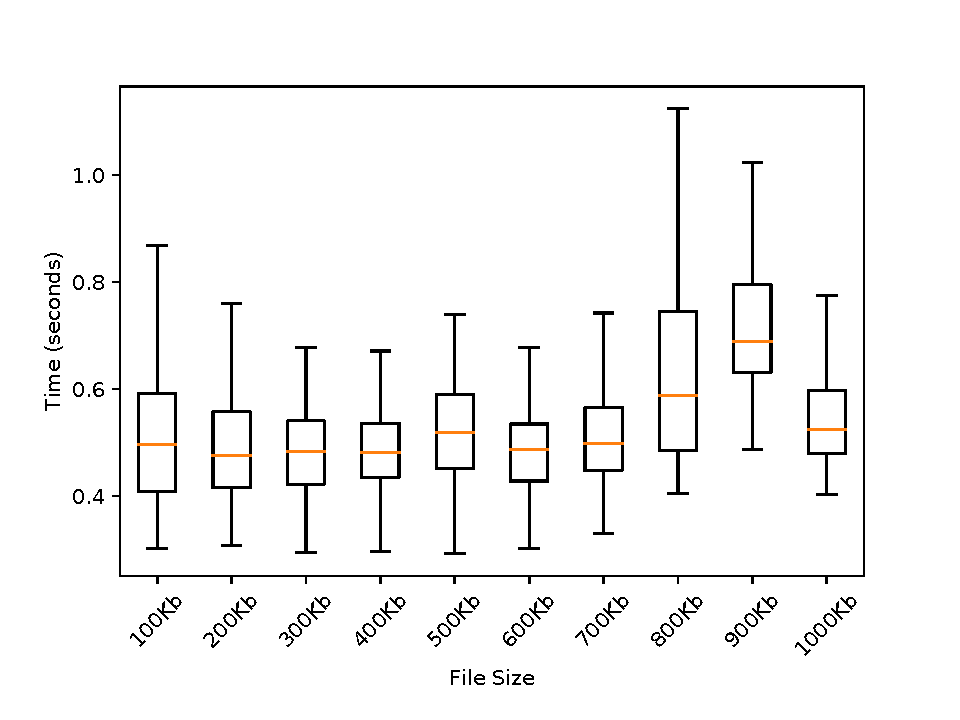
\includegraphics[width=\textwidth]{figures/results/gaia-writes.all/Build}
      \label{fig:gaia-write-build}
      \caption{Gaia Build performance.  Note that this includes the cost of
      fetching the existing manifest before constructing a new one.}
   \end{subfigure}
   \begin{subfigure}[b]{.8\textwidth}
      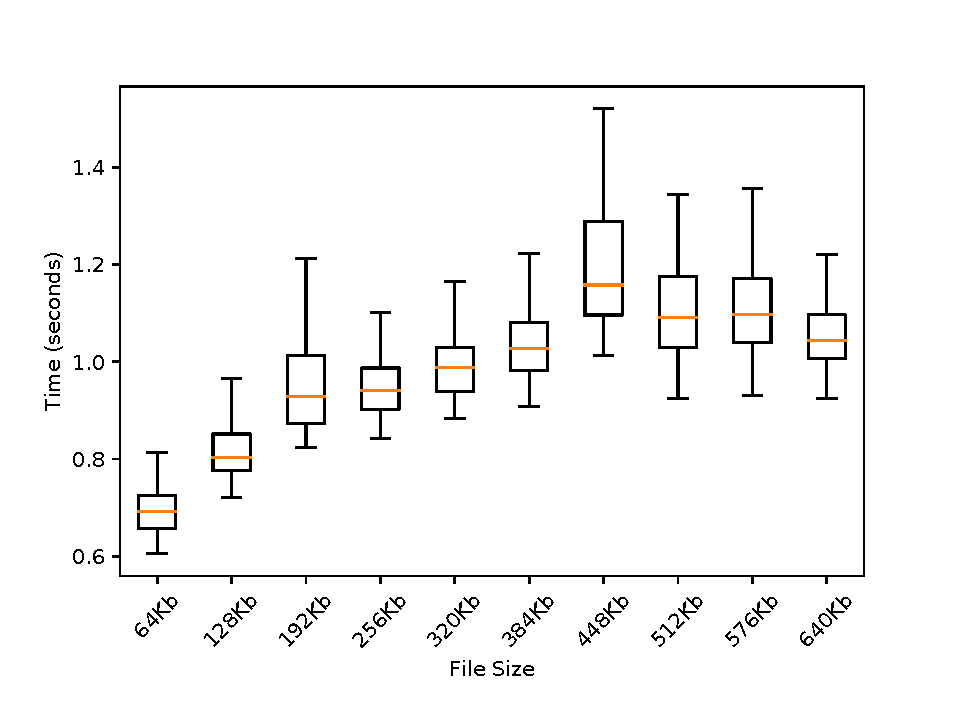
\includegraphics[width=\textwidth]{figures/results/gaia-writes.all/PushPublish}
      \label{fig:gaia-write-pushpublish}
      \caption{Gaia Push/Publish performance (both stages execute in parallel).}
   \end{subfigure}
   \label{fig:gaia-write-stages}
\end{figure}

Figure~\ref{fig:gaia-write-stages} shows the Build, Push, and Publish stage
perforamnces in Gaia.  In this test, the Build stage includes
the time taken to fetch a copy of the device manifest to update.  If the device
manifest is cached, then the Build stage is extremely fast---effectively the amount of
time taken to hash the data and insert it into a hash table and serialize the
hash table to a string for upload.

The Push and Publish stages run in parallel in Gaia by default, so their
measurements are combined.

\begin{figure}[htp!]
   \centering
   \caption{Box-and-wiskers plots of Gaia's write efficiencies.}
   \begin{subfigure}[b]{.8\textwidth}
      \includegraphics[width=\textwidth]{figures/results/gaia-writes.all/Efficiency}
      \label{fig:gaia-read-getmanifest}
      \caption{The cold efficiency, which includes the time taken to fetch the
      volume record over the network.}
   \end{subfigure}
   \begin{subfigure}[b]{.8\textwidth}
      \includegraphics[width=\textwidth]{figures/results/gaia-writes.all/Efficiency_cache}
      \label{fig:gaia-read-discover}
      \caption{The warm efficiency, which assumes the volume record is cached
      and excludes it from the mutate flow's running time}
   \end{subfigure}
   \label{fig:gaia-write-efficiencies}.
\end{figure}

This test calculated the efficiency of Gaia's write path in two ways---a ``cold
write efficiency'' which includes the cost of fetching the manifest in the Build
stage, and a ``warm write efficiency'' which excludes this step.  Including both
efficiency measures is valuable to developers because often times, the manifest
can be safely cached across writes.  Figure~\ref{fig:gaia-write-efficiencies}
reports both cold and warm efficiencies.  The efficiency of the write path
improves somewhat when the manifest can be cached across writes.

\subsubsection{Recommendations to Developers}

Developers have a few strategies available to alter the performance of writes in Gaia.
The specific strategies taken ultimately depend on the workload and data being
stored.

\hfill \break
\noindent{\textbf{Incremental Key Space Shard Writes}}
\hfill \break

Some applications may have a large key space, but only need to carry out a
key/value writes at a time.
The aggregation driver has an opportunity to reduce the amount of time and space that
need to be consumed to carry the write out by only writing the new key metadata.

If the application only wrote one value, then only one key in the manifest would
be altered.  The Build stage could be optimized to inspect the Gaia node's 
key space shard inbetween writes, only pass along the delta between writes
to the Push stage.

The Push stage would accumulate deltas from the Build stage, and combine them
into a single key shard in the backend storage service.  Then, a subsequent
Acquire step would continue to fetch the key space shard as expected.

The reason this is not the default behavior is because patching a record
efficiently requires the cloud service to support a ``range write''
API call, whereby the client specifies a byte offset and length as to where to
write the given data.  Most popular cloud storage providers do not support
this---they only allow clients to write whole records.  For these services,
a Push stage could not efficiently write key shard deltas, since it would need
to load the entire key shard, patch it, and store the entire updated key shard
on each write.  As such, this behavior would be added by developers in the
special case where they were using a suitable cloud storage provider.

\hfill \break
\noindent{\textbf{Write Batching}}
\hfill \break

Applications may not need all of their writes to be Published immediately.
Instead, a Publish can reflect many writes at once.  This would be allowed if
the application's storage semantics do not require all peers to see each others'
most-recent state.  This can lead to better overall performance for applications
that frequently overwrite the same key/value pairs---overwritten key/value pairs
would not need to be replicated.

Applications that have semantics compatible with write-batching can not only
realize better performance than the default behavior, but also take advantage of
client-side libraries that offer more expressive storage interfaces.
Examples include Compass~\cite{blockstack-compass}, which provides a
MongoDB-like interface, and \texttt{sql.js}~\cite{sql.js}, which provides a
client-side SQLite implementation.  Both of these libraries are easily used with
Gaia, provided that the application's storage semantics allow write-batching
(i.e. a Publish would take place in response to the application committing a
transaction in one of these APIs).  In fact, Compass was designed specifically
for Gaia by a third party contributor.

\subsection{Overheads in Syndicate}

Syndicate's default write strategy is make data as durable as possible. 
This is realized by the default behaviors of replicating all
manifests and blocks to all replica gateways in the volume in the
Push stage, and synchronously uploading the record's metadata to the Syndicate
MS in the Publish stage.

User gateways invoke the Build, Push, and Publish stages on write.
Since Syndicate is designed to process scientific workloads, it expects
multiple write-capable user gateways to be online at once.  However, it assumes
that user gateways usually (but not always) write to the same files that they
coordinate.  This is reasonable in practice, since scientific computing loads
are usually designed to run on many parallel computers which share as little
data with one another as possible.

In light of this, the default common-case behaviors of the Build, Push, and
Publish stages in Syndicate are to assemble a new manifest locally (Build),
replicate the manifest and blocks to all replica gateways (Push), and
synchronously upload the new metadata to the MS (Publish).  Push and Publish are
run automatically when a record is \texttt{close()}'ed, if the application does
not do so explicitly via a call to \texttt{fsync()}.  These are the default
behaviors of the user gateway carrying out the write is also the coordinator.

If the writer gateway is not the coordinator, then it enlists the
coordinator's help it carry out the write.  The writer's Push stage will first
replicate the new blocks, and then synchronously request that the coordinator
both Push a new manifest with the requested changes
and Publish new metadata that reflects it.

By default, replica gateways do not have any specialized aggregation driver
logic on the write path.
They simply accept chunks from user gateways, and replicate them with
their service drivers.

To summarize, the write overheads in Syndicate are as follows:

\begin{itemize}
\item \textbf{The time and space overheads of building a new manifest}.  By
default, a UG will encur a network round-trip when it Builds a new manifest for a record that
it does not coordinate.  In addition, the UG will incure a round-trip to
the MS to ensure that the new manifest it is modifying is fresh when executing
the default Build implementation.
\item \textbf{The time and space overheads of storing new metadata}.  The
record's coordinator will incur a network round-trip to the MS when Publishing
new data, and storing the new metadata incurs $O(1)$ extra space.  In the case
where the writer is not the coordinator, two network round-trips are incurred:
one to the MS and back, and one to the coordinator and back.
\item \textbf{The time and space overheads of storing a new manifest}.  The
record's coordinator will incur a network round-trip to each replica gateway to
store the new manifest, and a network round-trip from each replica gateway to
its underlying storage services.  This yields $O(g)$ round-trips, where $g$ is the number of
replica gateways.  The manifest size is $O(n)$ bytes for a record of $n$ bytes,
so replicating and storing it to all gateways takes $O(gn)$ time and space.
\item \textbf{The time overheads of storing blocks}.  Similar to manifests,
replicating a block takes two network round-trips (one for the replica gateway,
and one for the service).
\end{itemize}

\subsubsection{Measured Overheads}

The overheads of writing in Syndicate were measured for the same block sizes and
record sizes as reads:  records composed of 10 to 100 blocks (in intervals of 10
blocks) for a ``small'' block size of 1K and a ``medium'' block size of 10K.
The same UG, RG, and MS in the read test were used in the write test.
The total mutate flow performances are shown in
Figure~\ref{fig:syndicate-writes-total}.

\begin{figure}[htp!]
   \centering
   \caption{Box-and-whiskers plots of mutate flow performances in
   Syndicate, for file sizes between 10K and 100K and a block size of 1K.}
   \begin{subfigure}[b]{.8\textwidth}
      \includegraphics[width=\textwidth]{figures/results/syndicate-writes.1024.all/Total}
      \label{fig:syndicate-read-discover-1k}
      \caption{Syndicate mutate flow performance with 1K blocks}
   \end{subfigure}
   \begin{subfigure}[b]{.8\textwidth}
      \includegraphics[width=\textwidth]{figures/results/syndicate-writes.1024.all/Total}
      \label{fig:syndicate-read-acquire-1k}
      \caption{Syndicate mutate flow performance with 10K blocks}
   \end{subfigure}
   \label{fig:syndicate-writes-total}
\end{figure}

Despite the noisy measurements, the amount of time taken to write records of
these sizes grows linearly with file size.  For the 1K block measurement, the noise in the
measurements is mainly due to variations in the disk write performance and
chunk-writing scheduler in the UG.  For the 10K block measurement, the noise is
mainly due to the Push stage (i.e. there is more variance in uploading large
blocks).  This is visible in the Build, Push, and Publish
performances in Figures~\ref{fig:syndicate-build}, \ref{fig:syndicate-push}, and
\ref{fig:syndicate-publish}, respectively.

\begin{figure}[htp!]
   \centering
   \caption{Box-and-whiskers plots of the Build stage performance, for 1K and
   10K blocks.}
   \begin{subfigure}[b]{.8\textwidth}
      \includegraphics[width=\textwidth]{figures/results/syndicate-writes.1024.all/Build}
      \label{fig:syndicate-build-1k}
      \caption{Syndicate Build stage performance with 1K blocks}
   \end{subfigure}
   \begin{subfigure}[b]{.8\textwidth}
      \includegraphics[width=\textwidth]{figures/results/syndicate-writes.10240.all/Build}
      \label{fig:syndicate-build-10k}
      \caption{Syndicate Build stage performance with 10K blocks}
   \end{subfigure}
   \label{fig:syndicate-build}
\end{figure}

The Build step occurs within the UG.  In Syndicate, the Build step includes the
process of hashing the blocks and flushing them to a temporary storage location on
disk before it is replicated.  While the effect is hard to see here due to the 
small amount of data, the Build stage's time increases linearly with the amount
of data being written, since the manifest includes the hashes of all blocks
(Figure~\ref{fig:syndicate-build}).  The Build stage with 1K blocks compless in
less than 500 milliseconds, while the Build stage with 10K blocks takes less
than 750 milliseconds.

\begin{figure}[htp!]
   \centering
   \caption{Box-and-whiskers plots of the Push stage performance, for 1K and
   10K blocks.}
   \begin{subfigure}[b]{.8\textwidth}
      \includegraphics[width=\textwidth]{figures/results/syndicate-writes.1024.all/Push}
      \label{fig:syndicate-push-1k}
      \caption{Syndicate Push stage performance with 1K blocks}
   \end{subfigure}
   \begin{subfigure}[b]{.8\textwidth}
      \includegraphics[width=\textwidth]{figures/results/syndicate-writes.10240.all/Push}
      \label{fig:syndicate-push-10k}
      \caption{Syndicate Push stage performance with 10K blocks}
   \end{subfigure}
   \label{fig:syndicate-push}
\end{figure}

The Push stage replicates all blocks to the RG.  The Push stage times show linear
increases with the number of blocks (Figure~\ref{fig:syndicate-push}).
In the 1K block size case, the median Push stage
completes within 1.9 and 2.5 seconds.  In the 10K block size case, the median
Push stage completes within 3.5 and 8.1 seconds.

\begin{figure}[htp!]
   \centering
   \caption{Box-and-whiskers plots of the Publish stage performance, for 1K and
   10K blocks.}
   \begin{subfigure}[b]{.8\textwidth}
      \includegraphics[width=\textwidth]{figures/results/syndicate-writes.1024.all/Publish}
      \label{fig:syndicate-publish-1k}
      \caption{Syndicate Publish stage performance with 1K blocks}
   \end{subfigure}
   \begin{subfigure}[b]{.8\textwidth}
      \includegraphics[width=\textwidth]{figures/results/syndicate-writes.10240.all/Publish}
      \label{fig:syndicate-publish-10k}
      \caption{Syndicate Publish stage performance with 10K blocks}
   \end{subfigure}
   \label{fig:syndicate-publish}
\end{figure}

The Publish stage replicates the new manifest ID to the MS, as well as a
garbage-collection log.  Because the garbage-collection log data that the UG
replicates is proportional to the number of blocks written, it is expected that
the amount of time taken to replicate metadata will increase linearly with the
size of the write.

However, due to the facts that only at most 100 blocks are replicated and that
the size of a garbage-collection entry is 8 bytes, this linear relationship is
not visible.  Publish steps take between 640 milliseconds and 900 milliseconds
across both the 1K and 10K block size tests
(Figure~\ref{fig:syndicate-publish}).

\begin{figure}[htp!]
   \centering
   \caption{Box-and-whiskers plots of the efficiencies of Syndicate
   writes.}
   \begin{subfigure}[b]{.8\textwidth}
      \includegraphics[width=\textwidth]{figures/results/syndicate-reads.1024.all/Efficiency}
      \label{fig:syndicate-efficiency-1k}
      \caption{Syndicate write efficiency for 1K blocks.}
   \end{subfigure}
   \begin{subfigure}[b]{.8\textwidth}
      \includegraphics[width=\textwidth]{figures/results/syndicate-reads.10240.all/Efficiency}
      \label{fig:syndicate-efficiency-1k}
      \caption{Syndicate write efficiency for 10K blocks.}
   \end{subfigure}
   \label{fig:syndicate-write-efficiency}
\end{figure}

The write efficiencies of Syndicate are shown in
Figure~\ref{fig:syndicate-write-efficiency}.  As long as internal fragmentation
can be avoided, using larger block sizes drastically improves the system's
efficiency.

\subsubsection{Recommendations for Developers}

In addition to recommendations for aggregation driver developers for reads, some
performance enhancements can be devised for writes.  These strategies depend on
the workload and the nature of the data, which is why they are not included in
the default behavior.

\hfill \break
\noindent{\textbf{Write Coalescing}}
\hfill \break

A lot of workflows write data sequentially, and in bursts.
Developers can save a set of round-trips to the replica gateways
in the case where two sequential writes straddle a block boundary
by deferring replication of the straddled block.

\hfill \break
\noindent{\textbf{Replica Gateway Selection}}
\hfill \break

Developers are not required to replicate a chunk to all gateways.  It is
expected that in situations where there are multiple choices for a data store,
the aggregation driver will choose which chunk goes with which storage provider.
This can be done both to preserve end-to-end storage semantics, and to improve
write performance.

\hfill \break
\noindent{\textbf{Replica Gateway Chains}}
\hfill \break

Syndicate supports custom gateway types.  Developers can exploit this
to implement chain replication~\cite{chain-replication}~\cite{craq}, whereby a set of 
replica gateways are arranged into a sequence such that when receiving a chunk,
the gateway stores it and forwards it to the next gateway in the sequence.
User gateways would only need to forward chunks to the chain tip.  The tip would
have a ``replica gateway'' type, but the gateways in the chain would have a
distinct ``chain replicator'' type.

The aggregation driver would be written
such that each replica gateway and chain replicator gateway discover their
types and locations in the topology from the certificate graph.  The Push stage
for each gateway would use this knowledge to determine its next-hop gateway.
This strategy is generalizable to arbitrary store-and-forward topologies.

The performance advantage this would incur is that it would enable the same
degree of durability as replicating in parallel, but without the extra
round-trips from the user gateway.  User gateways located behind
underprovisioned network links would notice the improvement, since they would
not need to spend as much time pushing chunks through a local bottleneck.

\hfill \break
\noindent{\textbf{Chunk Patching}}
\hfill \break

If the workload exhibits random-write behaviors, one strategy developers can
emoploy is to implement a ``patching'' algorithm in their aggregation driver's
Push stage.  Instead of sending the entire chunk to a replica gateway, a user
gateway would send only the byte ranges and offsets to the replica gateways.
This would cut down on the data the replica gateway needs to send, even if the
block size in the volume was large.
The replica gateway would reassemble the patches into a block sometime before
the next read occurs---either eagerly as part of an internal
garbage-collection algorithm, or lazily as part of the \texttt{get\_chunk()} or
\texttt{serialize()} driver methods.

\section{Discussion}

Both Syndicate and Gaia add measurable overheads when compared to reading and
writing directly to cloud storage.  This should come as no surprise given the
designs of these two systems.

The overheads in both Gaia and Syndicate are due to three design factors:
all data is broken up and transmitted as blocks and manifests, all data
passes through one or more gateways en route to services that host it, and reads
and writes may incur an extra round-trip to the SDS system's metadata service.
The microbenchmarks presented here show that these overheads either increase the
time and space requirements by a constant factor, or are in a linear
relationship with the amount of data being read or written.  The fact that
the read and write efficiencies both increase with the size of the data indicates
that loading and storing the data to the underlying storage services are the
limiting factors to the system's performance.

The benefits to users and developers the systems offer cannot be overstated.
Using SDS systems has the same value proposition of using TCP/IP sockets instead of
layer-2 frames, or using filesystems instead of directly loading and storing
disk sectors.  While both SDS and these systems impose measureable overhead
and are less performant than the alternatives, the gains that users and
developers realize by using them outweight the performance loss.

The case for SDS-powered applications is becoming more and more apparent to even
non-academic and non-technical audiences.  Implementing featuers such as
end-to-end data privacy and data portability is straightforward in SDS, since
SDS systems already isolate applications from both the storage they use and the
trust relationships between users and organizations.  In fact, Gaia-powered SDS
applications like Graphite Docs and Stealthy have already been reported on in
mainstream media~\cite{graphite-wired}~\cite{washington-post-blockstack}, in
which these very features are touted as technical remedies to problems that
exist in Google Docs and Facebook Messanger, respectively.

\chapter{Related Work}
\label{chap:related-work}

The SDS approach described in this thesis
is synthesized from ideas from several different bodies of work.  Individual
concepts in SDS are based on time-tested design principles and engineering
techniques that have seen widespread usage.  Our contribution is
a new way to apply many existing principles in a coherent fashion
to address long-standing challenges in
the design of wide-area networked applications.

\section{Software-defined Storage in Industry}

% SDS 
Over the course of the development of this work, the term ``software-defined
storage'' has emerged as a marketing term in the software
industry with a different meaning than the one put forth here.
In the industry, SDS refers to software that implements some form of 
network-wide storage virtualization or storage emulation
in the context of a single organization (e.g. company or datacenter)~\cite{techcenter-sds-definition}.

Industry offerrings that refer to themselves as ``software-defined storage''
focus on implementing datacenter storage hardware as software, thereby
decoupling datacenter tenants and operators from specific vendors.  This is a
complementary to but fundamentally different problem from our work, which
focuses on preserving \emph{wide-area} applications' storage semantics in the face of
changes to underlying storage systems.  Our work addresses the problem of
preserving stoarge semantics across multiple organizational boundaries, where
users initially do not trust one another or organizations that they are not a
part of.

\subsection{Virtual Block Devices}

One category of industry offerings that refers to itself as ``software-defined
storage'' focuses on implementing programmable block devices.
Recent work on datacenter storage networks have focused on providing SDN-like
abstractions to manage VM disk I/O queues.  In
IOFlow~\cite{ioflow}, virtual block devices
are mapped into VMs as virtual hard drives, and the datacenter implements a
centralized storage control plane and distributed data plane to shape I/O traffic to and
from storage servers.

Some storage vendors have begun to refer to their existng iSCSI, NAS, and SAN offerrings as
``software-defined storage''~\cite{computerweekly-storagebuzz}.  In particular,
they tout the ability to run the storage network controllers in
software (whereas previously, they had been implemented on dedicated hardware).

Another work that refers to itself as software-defined storage
is software-defined flash~\cite{sdf-baidu}, where
datacenter applications interact with solid-state disks (SSDs) via a
software-defined flash controller.  This work focuses on improving utilization
of the hardware by allowing the application to directly control aspects of the
hardware that are typically left to the device driver or firmware (i.e. I/O scheduling,
channel utilization, provisioning, etc.).

\subsection{Storage System Emulation}

Other industry offerings that refer to themselves as ``software-defined storage''
focus on emulating existing storage systems, instead of specific pieces of
hardware.  This allows tenants to move from one datacenter to another without having to
rewrite the storage interfacing logic.  For example, industry offerings exist to
provide compatibility with NFS, CIFS, SMB, and Amazon S3 (contemporary examples include
Veritas~\cite{veritas}, Scality~\cite{scality}, Acronis~\cite{acronis}, and
Lenovo~\cite{lenovo}).

Our work on SDS implements storage system emulation
through aggregation drivers, and works across multiple organizations and
networks.

\subsection{Storage Abstraction and Virtualization}

Cloud storage gateways~\cite{gartner-cloud-storage-gateway} are recent type of
network appliance that refers to itself as ``software-defined storage.''
They allow an organization to apply certain data management
policies on organization-originated data bound for cloud storage.  These
policies include transparent compression, deduplication, encryption, access
logging and so on.

Our wide-area SDS gateways act as ``virtual'' cloud storage gateways
(after a fashion) in that they apply local data transformations (in the form of
an aggregation driver stage).  Unlike cloud storage gateways, SDS gateways exist
entirely in software, and can be provisioned, duplicated, migrated,
reprogrammed, arranged in a particular network topology on-the-fly.

Software compatibility librares like Apache libcloud~\cite{libcloud} and various
storage-specific userspace
filesystems~\cite{s3fs}~\cite{dropbox-client}~\cite{google-drive-fs} try to
provide a uniform interface for accessing disparate cloud storage resources.
This is equivalent to what service drivers do in SDS.  These systems only provide a uniform
\emph{syntactic} interface (i.e. a filesystem), but have different semantics.

\section{Operating System Storage Principles}

SDS isolates application design from both the syntactic and semantic interfaces
of underlying storage systems, and facilitates code-resuse by allowing
its components to be composed in a pipeline-like fashion.  These are extensions of
well-established operating system design principles.

\subsection{Operating System Storage Design}

The designs of virtual filesystem abstractions in various points of UNIX's evolution
~\cite{vnodes-sun-1986}~\cite{netbsd4.4-vfs-1995}~\cite{plan9-filesystem}~\cite{freebsd-design-book}
address this concern.  Like SDS, they introduce two layers of indirection
---a set of filesystem drivers that overlay a set of block device drivers---to
isolate single-device semantics from cross-device semantics.  This is analogous
to our concept of service drivers and aggregation drivers being logically
distinct abstraction layers.

The presence of two layers of indirection can also be found in the storage
architectures of other multi-user non-UNIX
operating systems like VMS~\cite{vms-driver-model}, Microsoft
Windows~\cite{ms-windows-driver-model}, and IBM System z~\cite{ibm-vsams}.
We believe this is an emergent design pattern in storage systems with multiple
back-ends, and our work in SDS echos this pattern.

One task performed by SDS systems is storage virtualization.  Synthesizing
logical volumes from multiple devices~\cite{lvm} has been a mainstay in most UNIX-like
operating systems, and hierarchical storage management~\cite{hsm} has been used
in production in mainframes for decades.

\subsection{Composible Software Systems}

SDS allows developers to construct complex storage systems by composing
unrelated stages of different aggregation drivers into a single driver.
This design principle is similar to the UNIX design philosophy~\cite{unix-design-philosophy},
stackable filesystems~\cite{FUSE-stack}, network function virtualization systems
like ONOS~\cite{onos},
and programmable network processors like the Click modular router~\cite{click-modular-router}.

SDS aggregation drivers are constructed by chaining together a sequence of
unrelated but reusable stages to form a program that controls the system's
end-to-end storage processing.  This is analogous to how UNIX programs are built
by chaining together unrelated programs into pipelines, how stackable
filesystems can be chained together to implement complex storage semantics, how
how Click router components can be chained together to implement complex
packet-processing programs, and how network functions are chained together to
implement complex network-wide processing.

In all cases, the developer has a global,
complete view of the program's implementation, and can easily alter the
program by swapping modules out.  SDS extends this idea to
multi-user, multi-network settings, where parts of the
aggregation driver operate in separate organizations.

\section{Secure Software Deployment}

A major concern in the operation of SDS systems is the ability for volume owners
to specify and upgrade drivers at runtime.  This allows them to preserve the
storage semantics of their volumes in face of changes in the underlying
services.  But in order to do so, SDS systems must offer a way to securely
deploy new driver code at run-time, without interrupting the running system.

\subsection{Secure Package Deployment}

The concerns addressed by prior work like Stork~\cite{stork},
Raven~\cite{raven}, and The Update Framework~\cite{TUF}
revolve around ensuring end-to-end software authencitity and
freshness, so that the remote hosts deploy the code the owner specifies without
having to trust any intermediate repositories.
SDS must address this concern as
well in the deployment of driver code and configuration.  Our work
operates under the additional constraint that upgrades must be atomic with
respect to all ongoing application-level operations.

\subsection{Secure Remote Execution}

The aggregation driver only executes successfully if all of its stages
execute successfully, even though they run in separate organizations.  This
introduces the problem of verifying that the remote processor executed the code
as prescribed.  Prior work in secure remote execution focuses on new
computational techniques, like implementing
homomorphic encryption~\cite{homomorphic-encryption}, preserving auditable
execution traces~\cite{truebit}, or relying on trusted hardware extensions in
the remote computers~\cite{intel-sgx}.

SDS gateways complement this prior work in multi-host, multi-network settings by
ensuring that each gateway has a coherent view of the other gateways invoking
its driver code.  A data flow only executes if all affected gateways can first
verify that they each know what code each other gateway is running.  It is
possible to construct SDS gateways that employ a secure computation technique
like prior work, and in doing so, arrive at a data flow processing algorithm
that can be audited end-to-end by concerned users.

\section{Software-defined Networks}

Software-defined networking (SDN) addresses similar types of problems for
network policy as SDS addresses for data policy.  SDS builds on several design
techniques pioneered in SDN systems.

\subsection{Control and Data Planes}

Early SDN systems like
4D~\cite{4D} and Ethane~\cite{ethane} introduced the concept of separating a
distributed data-processing plane from a logically-central control plane.
This allowed SDN operators to specify top-down, globally-scoped policies for controlling
network traffic, a key innovation over earlier work in active
networking~\cite{sdnhistory}.  SDS applies this concept by
separating data flow processing from configuration management, whereby the
volume owner operates the logically-central control plane for the
volume by manipulating a certificate graph.

Another key concept introduced by 4D is the notion of
dedicated subsystems for discovery of network elements and rule dissemination to
them.  SDS's use of a self-sovereign identity system and certificate graph
addresses the same kinds of problems, but for users and gateways instead of network
elements.

SDN encourages open interfaces between its control and data planes.
For example, the OpenFlow specification~\cite{openflow} describe interfaces for
network elements to implement in order to participate in an SDN system.
This removes a barrier to innovation by allowing control planes and data planes
to be implemented independently, leading to a proliferation of network operating
systems~\cite{ONOS}~\cite{NodeOS}~\cite{NOX}.

SDS extends this concept for
storage by encouraging the development of many different type of gateways, which
can be tailored to individual applications while remaining compatible with an
existing SDS system.  We have leveraged this property to implement email-specific replica
gateways on top of Syndicate, for example.

\subsection{Ease of Programmability}

More recent work in SDN programmability, such as Frenetic~\cite{frenetic} and
Pyretic~\cite{pyretic}, focuses on allowing developers to write a global flow
control program in a familiar language that compiles into individual flow rules.
We have taken a similar approach in the design of Syndicate's aggregation
drivers, whereby a single driver program is automatically distributed and
executed piecemeal across all of the volume owner's gateways.

\section{Peer-to-peer Storage}

SDS systems distribute data chunks in a peer-to-peer fashion, but use
a logically central metadata service to discover and route requests.  In
addition, they employ a ``trust-to-trust'' user discovery
layer~\cite{trust-to-trust principle} which SDS elements use to bootstrap trust
in one another.  Prior works in distributed storage systems have faced similar
challenges to the ones that necessitated these SDS design elements, but have
addressed them in different ways.

\subsection{Content Discovery}

Content discovery is an important aspect of distributed storage design.
Prior work in scalable distributed storage systems~\cite{berkeley-xFS}~\cite{farsight}~\cite{zebra}~\cite{spritefs}~\cite{glusterfs}~\cite{lustre}
has shown the utility of implementing separate metadata servers from data
servers.  This helps system operators to better manage access control and
consistency by placing the logic to do so within one system component.
SDS systems employ a metadata service to achieve the same end, but
such that metadata servers are not part of the trusted computing base.
The key differences between prior work and this work on SDS are that (1) that the metadata
service is \emph{not} trusted, and (2) SDS elements may be programmed to
validate the index via application-specific criteria.

In wide-area systems that span multiple organizations, a key difficulty with
addressing content discovery is ensuring that the system can operate under
organizational churn.  The solutions depend on who manages the content discovery
mechanism.

\subsection{Single-stakeholder Content Discovery}

Wide-area storage systems like Oceanstore~\cite{oceanstore}, Pond~\cite{pond},
and Bonafide~\cite{bonafide} implement content discovery by relying on a
federation of BFT nodes, which perform write admission control and write
serialization.  While they are all able tolerate the failures of other storage
elements, the users of these systems do \emph{not} participate in content
discovery and instead trust the federation to not be faulty.

SDS systems like Syndicate offer a more flexible approach.  While Syndicate
relies on a central metadata service for content discovery, the service is not
trusted.  Each application, through the use of an aggregation driver, can
program its volumes to validate system metadata in arbitrary ways.  This allows
the application to seamlessly control how much trust it places in metadata
services outside of its control.  For example, in the limit
the set of Syndicate gateways can maintain their own replicated log of metadata
writes through their aggregation driver,
and use the log to monitor the metadata service for faults.

\subsection{Multi-stakeholder Content Discovery}

Prior wide-area storage systems like Shark~\cite{shark}, CoralCDN~\cite{coral}, Vanish~\cite{vanish},
OpenDHT~\cite{opendht}, and BitTorrent~\cite{bittorrent} are designed with
\emph{multi-stakeholder} content discovery mechanisms.  Anyone can stand up additional
nodes to help with content discovery.  This is also the approach taken by Gaia.

A key improvement in multi-stakeholder content discovery systems offered by SDS
is the use of a blockchain as a shared source of truth between storage elements.
All of the aforementioned prior works rely on DHTs or DSHTs~\cite{dsht} in order to
scale the number of records, and work by distributing routing information
evenly across a number of hosts while tolerating node churn and supporting
fast queries.

The drawback with this approach is that they are vulnerable to Sybil
attacks~\cite{sybil-attack} and route-censorship
attacks~\cite{dht-route-censorship}.  This can cause to a loss of routing state,
and can possibly cause invalid or malicious routing state to be used.
Gaia avoids these problems by ensuring each node has a 100\% replica of the
routing state, and ensures that the state size grows at a fixed rate by relying
on a public blockchain as a rate-limiter.

\subsection{User Authentication}

Peer-to-peer systems are often multi-user systems.  To support multiple users,
they need to perform some form of user discovery and authentication.
Most network filesystems systems that run within a single organization (like
NFS~\cite{nfs} and GFS~\cite{gfs}) use a trusted, centralized user directory,
which allows users and administrators to enumerate user accounts and assign them
easy-to-remember names without name collisions.
Federated filesystems like AFS~\cite{afs} and Farsight~\cite{farsight} use a
trusted, existing public-key infrastructure to discover users in a similar
fashion.

Other systems try to do without a centralized user directory, but at the expense
of removing human-friendly user identifiers.  For example,
SFS~\cite{sfs} echews user enumeration by addressing this problem with
self-certifying paths, where users are identified by public keys.
Others like WheelFS~\cite{wheelfs} punt on user discovery altogether, and
require each operator to curate the public keys of trusted users out-of-band.

By relying on a self-sovereign identity system, SDS systems allow users to
discovery each other's public keys without a centralized user directory, and
without introducing human-unfriendly names.  Certain PKI systems like
attribute-based encryption~\cite{abe} try to enable this, but have the significant
drawback that each user must re-key if a single private key is compromised.

\section{User-defined Storage Semantics}

Different applications need to make different trade-offs in their storage.  To
accomodate this, prior work has provided
control points to help them make these trade-offs.  SDS systems take
this idea to its logical conclusion, where the application itself specifies a
portable, reusable driver that defines its end-to-end semantics.

In their simplest forms, systems that offer user-defined consistency do so by
allowing the user to choose from a handful of built-in semantics that all reads
and writes to the data will follow.  This includes systems like
WheelFS~\cite{wheelfs}, PRACTI~\cite{practi}, and
Bayou~\cite{bayou}, where the user can tag files and sessions as needing to
adhere to a certain consistency models have a certain degree of
durability.

Some storage systems try to resolve write conflicts by deferring to user
decisions.  These include version control systems like
subversion~\cite{subversion} and git~\cite{git}, and file storage systems like
Dropbox~\cite{Dropbox}.

Other storage systems like Coda~\cite{coda}, COPS~\cite{cops}, and
Ori~\cite{ori} allow the user to supply a conflict-resolution algorithm for
handling conflicts.  The algorithm is later used by the system in order to
resolve conflicts between replicas.

Systems that need high availability or high durability allow clients to choose
replica placement.  These include programmable CDNs like
CloudFlare~\cite{cloudflare} and Akamai~\cite{akamai}, as well as
high-availability cloud storage like S3~\cite{s3}.  Open-membership storage
layers that offer this include BitStore~\cite{bitstore} and Storj~\cite{storj}.

In the context of SDS systems, developers realize systems that address
\emph{all} storage concerns within a single storage element---the aggregation
driver.  This allows them maximum flexibility in addressing storage concerns.
SDS helps developers manage the associated complexity and development overhead
of doing so by providing an aggregation driver specification that facilitates
component reuse and piecemeal deployment.

\section{Applications}

We described three sample SDS-powered applications, all of which have been
implemented in prior work but with significant constraints.

\subsection{Encrypted Email}

PGP~\cite{pgp} has long been the ``gold standard'' for encrypted communication
over email.  It works by allowing users to send and receive encrypted messages
over SMTP.  However, multiple usability
studies~\cite{why-johnny-cant-encrypt}~\cite{why-johnny-still-cant-encrypt}~\cite{why-jonny-still-still-cant-encrypt}
have shown that users have a hard time interacting with cryptographic key pairs.
Email clients like Enigmail~\cite{enigmail} and Mailvelope~\cite{mailvelope}
attempt to allieviate some usability problems, but ultimately require users to
actively participatein key management and key discovery.  All PGP-based email
requires both the sender and recipients to participate in order to realize
message confidentiality and authenticity.

Our SDS-powered email application differs from prior work in that it removes the
need for humans to manage keys.  In doing so, we provide a user experience
comparable with Webmail.  The underlying SDS gateways automatically encrypt and
decrypt messages on endpoints, and provide multiple options for communicating
with legacy SMTP email users.

\subsection{Groupware}

Software that helps groups of users work on a shared task has been a significant
computer application since the late 1980s, with many early works focusing
on various ways to allow clients to interact with shared state on a server~\cite{readings-in-groupware}.
Many groupware applications, such as video-conferencing, chat rooms,
and document-sharing have subsequently been realized as Web applications.
Examples today include Microsoft Live~\cite{microsoft-live},
Docs~\cite{google-docs}, and Slack~\cite{slack}.

An architectural mainstay of most groupware systems is that they follow a client-server model.
The users run the client software on their computers (e.g.
as a Web page in a Web browser in contemporar systems) to interact with shared state hosted on one or
more servers.  Clients are not assumed to be reliable, and do not host any
authoritative state.  Instead, servers store the authoritative state of the system and
present clients with views of it.

What this means for groupware implementations is that most of the application's business logic runs on the
servers.  This is necessary in order to address global data management
concerns, such as access controls, concurrency handling, and
replication.  Since only the servers process operations on authoritative state, only
the servers are in a position to handle these concerns.  In doing so, groupware
servers pose a single point of failure---if a groupware server fails, clients
cannot interact with their data.

Gaia avoids this issue by separating the business logic from the storage logic.
Gaia still provides groupware applications with the client-server computing model,
but such that the role of the server is reduced to loading
and storing opaque blobs of data.  Gaia instead
moves application business logic into an aggregation driver, which can be
deployed, upgraded, and migrated across a dynamic set of gateways at runtime.
This provides a degree of operational flexibility not seen in prior groupware
implementations---a volume owner can transparently migrate the groupware from
one storage provider to another (to tolerate changes in service providers),
and from one gateway to another (to tolerate changes in trust relationships and
changes in host availability).

\subsection{Scientific Data Set Staging}

Related work on sharing scientific data across multiple networks includes
work on dedicated sharing and transfer services like Globus~\cite{globus},
hosting data in highly-available datacenters like ABoVE~\cite{nasa-above} and
Cyverse~\cite{cyverse}, and relying on an array of network caches to distribute
data from one data origin to many downstream readers (like
CernVMFS~\cite{cernvmfs}).

Scientific data transfer services allow labs to explicitly share and copy
data from one site to another.  Globus allows scientists to pipe data between
servers that the requester can access, and allows scientists to share data from
commodity cloud storage to external data consumers.  Like Globus, Syndicate
encourages reusing commodity cloud storage services for hosting data, and
leverages existing identity management services to authenticate data and
transfer requests between organizations.

We are not the first to propose using a network of commodity caches to help
distribute scientific data.  CernVMFS~\cite{cernvmfs} allows scientists at CERN
to share data with the world.  CernVMFS implements a catalog service that
functions like the Syndicate MS and AG in that it provides an index over the
available datasets, which can be fetched out of band and used to read the data
itself through the caches.

Our work extends this concept by supporting reads and writes while preserving
cache coherency.  Unlike CernVMFS, we allow the upstream datasets to be written
to at runtime, while there are ongoing reads.  Our AG and MS allow readers to
discover the latest data without having to rely on consistency hints from the
caches (such as Etags or Last-Modified HTTP headers).

\chapter{Conclusion}
\label{chap:conclusion}

Wide-area applications that leverage commodity infrastructure are difficult to
keep running in the face of changes in the underlying services.  Services can go
offline, services can change their APIs and storage semantics, and services can
fall outside the trust domains of their users.

We address these problems with wide-area software-defined storage.  By giving
developers the ability to implement their storage semantics as a first-class
storage element, we allow applications to tolerate changes in the underlying
services without requiring a patch each time.  In addition, we reduce the
problem of keeping many applications compatible with a single services to making a
service compatible with the software-defined storage system, instead of patching
each application.

We present the design space of wide-area software-defined storage, and
distilled several design principles for building such systems.  We showed the
feasibility of designing real-world SDS systems by creating two
implementations---Gaia and Syndicate.  Both systems allow applications to
leverage commodity cloud services in the face of changes to both the service API
and changes to the trust relationships users have with them.

To demonstrate the feasibility of constructing SDS-powered applications, we
present the design and implementation of three real-world applications:
end-to-end encrypted Webmail, decentralized groupware, and CDN-accelerated
scientific data staging.  In all three applications, we show how the ability to
define an aggregation driver allows us to solve several hard problems that have
plagued prior systems.

We give microbenchmarks and early performance numbers for our SDS prototypes and
sample applications.  We show that the overhead of the SDS system is acceptable,
since it does not affect the sample applications' usability.
Gaia, Syndicate, and our sample applications have all been released as
open-source~\cite{blockstack-core}~\cite{syndicate-storage}~\cite{syndicatemail}~\cite{todo-list}~\cite{blockstack-browser}~\cite{syndicate-sdm}~\cite{syndicate-containers}.




% Make the bibliography single spaced
\singlespacing
\bibliographystyle{plain}

% add the Bibliography to the Table of Contents
\cleardoublepage
\ifdefined\phantomsection
  \phantomsection  % makes hyperref recognize this section properly for pdf link
\else
\fi
\addcontentsline{toc}{chapter}{Bibliography}

\bibliography{bibdata}

\end{document}
